\documentclass[11pt,letterpaper]{book}

%\usepackage[dvips]{graphicx} 
\usepackage{graphicx} 
\usepackage[small,bf,hang]{caption2}
\usepackage{amsmath}
\usepackage{multicol}
\usepackage{cancel}
\usepackage{cmap}        % Added 11/19/14 by ML.  Insures that ligatures
                         % will be recognized in most pdf viewer searches
                         % when compiled with pdflatex
\usepackage{supplement}  % local style file, defines example env



%%DIF PREAMBLE EXTENSION ADDED BY LATEXDIFF
%%DIF UNDERLINE PREAMBLE %DIF PREAMBLE
%\RequirePackage[normalem]{ulem} %DIF PREAMBLE
%\RequirePackage{color}\definecolor{RED}{rgb}{1,0,0}\definecolor{BLUE}{rgb}{0,0,1} %DIF PREAMBLE
%\providecommand{\DIFadd}[1]{{\protect\color{blue}\uwave{#1}}} %DIF PREAMBLE
%\providecommand{\DIFdel}[1]{{\protect\color{red}\sout{#1}}}                      %DIF PREAMBLE
%%DIF SAFE PREAMBLE %DIF PREAMBLE
%\providecommand{\DIFaddbegin}{} %DIF PREAMBLE
%\providecommand{\DIFaddend}{} %DIF PREAMBLE
%\providecommand{\DIFdelbegin}{} %DIF PREAMBLE
%\providecommand{\DIFdelend}{} %DIF PREAMBLE
%%DIF FLOATSAFE PREAMBLE %DIF PREAMBLE
%\providecommand{\DIFaddFL}[1]{\DIFadd{#1}} %DIF PREAMBLE
%\providecommand{\DIFdelFL}[1]{\DIFdel{#1}} %DIF PREAMBLE
%\providecommand{\DIFaddbeginFL}{} %DIF PREAMBLE
%\providecommand{\DIFaddendFL}{} %DIF PREAMBLE
%\providecommand{\DIFdelbeginFL}{} %DIF PREAMBLE
%\providecommand{\DIFdelendFL}{} %DIF PREAMBLE
%%DIF END PREAMBLE EXTENSION ADDED BY LATEXDIFF



\begin{document}

\frontmatter

% \begin{titlepage}
\begin{center}

\newfont{\ssvl}{cmdunh12 scaled 4500}
\newfont{\ssvm}{cmdunh12 scaled 3000}
\newfont{\ssl}{cmdunh12 scaled 3000}
\newfont{\ssm}{cmdunh12 scaled 2000}

{\ssvl P}{\ssvm HYSICS}\hspace{0.2in}{\ssvl 211}

\vspace{1.2in}

{\ssl A}{\ssm DDITIONAL PROBLEMS}\\
\vspace{0.3in}

{\ssl \&}
\vspace{0.2in}

{\ssl S}{\ssm UPPLEMENTARY}\\
\hspace{0.3in}

{\ssl R}{\ssm EADING}

%\vspace{0.9in}
%{\ssl P}{\ssm ART}~~~~{\ssl I}

\vspace{1.2in}

{\ssl F}{\ssm ALL}\hspace{0.15in} {\ssl 2010}

\end{center}
\end{titlepage}

\mbox{}
\vspace{7in}

\noindent
Copyright \copyright\ 2016 by the Bucknell University Department of
Physics \&\ Astronomy.
All rights reserved. 

\tableofcontents


\mainmatter

\input{additional_problems/additional_problems}

\input{numerical_integration/numerical_integration}

\input{nonconservative}

\input{basic_postulates_of_relativity/basic_postulates_of_relativity}

\chapter{Relativistic Spacetime}
\label{chapter:relativistic_spacetime}

%\section*{Objectives}
%\begin{objectives}
%\item Be able to calculate a spacetime interval between two events,
%  and classify the interval as space-like, time-like or light-like.
%  Use these classifications to determine whether or not the two events
%  could be causally linked.
%\item Be able to use the invariance of the interval to relate distance
%  and time intervals in one reference frame to those in a different
%  frame.
%\item Be able to draw and/or interpret a spacetime diagram, and use
%  this diagram to determine temporal and spatial ordering of events,
%  including whether or not events are simultaneous or at the same
%  location.
%\end{objectives}

\section{Introduction}


The previous chapter introduced the basic ideas of relativity along
with some of the most dramatic implications of the theory.  But the
predictions of time dilation and length contraction are merely special
cases of a much broader theory.  In this chapter, we discuss the idea
of spacetime, which blends time and space together.  We introduce the
spacetime interval, a quantity that is one of the fundamental
invariants in relativity, and we use this interval to relate distance
and time measurements made in different reference frames that 
are moving with respect to each other.  We also introduce
spacetime diagrams, which provide a graphical way of illustrating
relativistic phenomena, particularly the relativity of simultaneity.
    
%We also develop the relativistic velocity transformation formulas,
%which allow us to compute a particle's velocity in one inertial frame
%if we know the particle's velocity in another inertial frame.

\section{Spacetime intervals}

\label{sec:spacetime_intervals}

As we saw in Chapter \ref{chapter:relativityI}, observers in different reference frames
disagree about time and distance measurements.  But there are a few
quantities referred to as invariants upon which all observers agree
regardless of their reference frames.  One of these invariants was
discussed in the previous chapter; namely, the invariance of the speed
of light in a vacuum.  It turns out that distance and time can be
folded together to make another invariant, referred to as the
invariant spacetime interval $I$, defined by

\begin{equation}
I^2 \equiv \left(c\Delta t\right)^2 - \left(\Delta x\right)^2.
\label{eq:intervaldef}
\end{equation}
Note that $I^2$ can be positive, zero, or negative.  If $I^2$ is
positive, then the interval is called {\em time-like\/}  since the first term
--- with $\Delta t$ in it --- dominates.  Similarly, negative values
of $I^2$ correspond to {\em space-like\/} intervals, and if $I^2 = 0$, the
interval is called {\em light-like\/}.  Qualitatively, an event is light-like
if a pulse of light could travel directly between the two events.
This can be seen from Eq.~(\ref{eq:intervaldef}): if $I^2 = 0$, then
\begin{align}
0 &= \left(c\Delta t\right)^2 - \left(\Delta x\right)^2  \nonumber \\
\Rightarrow \Delta x &= \pm c \Delta t,
\end{align}
as would be expected for a pulse of light traveling a distance $\Delta
x$ in a time $\Delta t$.

Two events could be {\em causally-linked} (i.e., event A actually
causes or contributes to event B) if the spacetime interval between
them is either light-like or time-like.  In fact, for time-like
spacetime intervals, the interval is the proper time (multiplied by $c$).  
If two events are separated by a space-like interval, then no 
information can travel between the two events since it would require 
superluminal ($|v| > c$) information transmission, and nothing 
(especially information) can travel faster than light relative to 
any observer.  So events {\em can't} be causally linked if the square 
of the spacetime interval between them is negative.


\begin{example}{Causality and intervals}  
  In the year 2055, a father and his daughter are watching the 5$^{\rm
    th}$ game of the National League Divisional Series from a Moon base at the Sea of
  Tranquility.  The Washington Nationals lead the St. Louis Cardinals by a run with 2 outs 
  in the bottom of the ninth
  inning, but the bases are loaded. The daughter sneezes and then watches in horror as
  $2.0\units{s}$ later Drew Storen, Jr., of the Nationals throws
  a wild pitch that not only walks in the tying run but also allows St. Louis to
  score the winning run. Distraught, the
  daughter bursts into tears. ``What's wrong?'' her father asks.
  ``It's my fault that the Nats lost!  My sneeze caused Storen to throw
  that wild pitch!'' What argument should the father use to assure his daughter
  that she is not personally responsible for yet another
  heart-breaking Nats playoff loss?  

\solution The father should first point
  out that the distance between the Earth and Moon is $3.84\times
  10^8\units{m}$, or $1.3\units{lt-s}$.  So, if the father/daughter
  received the TV signal of the strikeout $2.0\units{s}$ after the
  sneeze, in their reference frame it must have actually occurred only
  $0.7\units{s}$ after the sneeze.  (It takes the TV signal
  $1.3\units{s}$ to make it from the Earth to the Moon.)  Now, the
  father should calculate the spacetime interval:
\begin{align}
I^2 &= \left(c\Delta t\right)^2 - \left(\Delta x\right)^2 % \nonumber \\
    = (1\units{lt-s/s}\times 0.7\units{s})^2 - 
                    (1.3\units{lt-s})^2 % \nonumber \\
    = -1.2\, (\mbox{lt-s})^2 \nonumber 
\end{align}
So, the father should pat the daughter on the head and say, ``So,
you see honey ---  you can't have caused Storen to throw that wild pitch 
because the spacetime interval between your sneeze and his strikeout
is a space-like interval!''\footnote{By the way, we originally wrote this
problem about the Red Sox when they hadn't won a World Series in over 80
years. The following year, they won the World Series. And {\bf that} is a
{\em time-like} interval, so, yes, we do take credit for the Red
Sox victory.}
\footnote{And then we switched the example to one with the Cubs because,
well, it didn't work for the Red Sox anymore, and we figured, "Well, we'll be
able to use this example for {\bf decades} because the Cubs will never win
the World Series!" But the Cubs messed that up this past year. (Also a
time-like interval, so we take credit for the Cubs World Series
championship, too.) Fans of
the Nationals in PHYS 211 requested that we use the Nats now in this example.}
\label{example:causality-intervals}
\end{example}

Don't worry about the fact that $I^2$ is negative for space-like
intervals.  The definition of $I^2$ in Eq.~(\ref{eq:intervaldef}) is
chosen so that for time-like intervals, the interval $I$ itself is the
proper time (multiplied by $c$), which is convenient for our purposes.  
But the interval could have equally been defined as 
$I^2 = \left(\Delta x\right)^2 - \left(c \Delta t\right)^2$, 
in which case $I^2$ would be negative for
time-like intervals (some authors do, in fact, define $I^2$ this way).
In fact, some physicists define two different intervals: $I^2 =
\left(c\Delta t\right)^2-\left(\Delta x\right)^2$ for time-like
intervals and $I^2 = \left(\Delta x\right)^2-\left(c\Delta t\right)^2$
for space-like intervals.  We will stick with Eq.~(\ref{eq:intervaldef}).

As stated earlier, $I^2$ is an invariant --- observers in different
reference frames will agree on the value of this interval for any two
events:
    
\begin{equation}
I^2 = \left(I^\prime\right)^2,
\end{equation}
or

\begin{boxiteq}{
\begin{equation}
\left(c\Delta t\right)^2 - \left(\Delta x\right)^2 = 
              \left(c\Delta t^\prime\right)^2 - 
     \left(\Delta x^\prime\right)^2.
\label{eq:interval-invariance}
\end{equation}
}
\end{boxiteq}

\noindent This is important for several reasons.  First, the
invariance of the interval helps to further clarify the intimate
connection between distance and time in relativity.  Any disagreements
between different observers about the time interval between events
must be accompanied by a corresponding disagreement in the distance in
order to keep the interval invariant.  Second, if an interval is
space-like or time-like or light-like as viewed in one reference
frame, then it is the same kind of interval as viewed in any reference
frame.  This makes sense: if two events cannot be causally-linked in
one reference frame, for instance, it would be nonsensical to think
that they would be causally-linked as observed by someone in a
different reference frame.  Finally, the interval can be used to
determine how events are viewed in one reference frame, given
information in a different frame.  As an example, we refer back to a
problem from the previous chapter.


\begin{example}{Using the interval} 
  A spaceship crew wants to make the trip from Earth to Alpha Centauri
  in only 2.0 years as measured by clocks on board their spaceship.\\
  (a) How long does the trip take according to Earth-frame observers?
  (b) How fast must the astronauts travel relative to Earth?
  \solution For problem \ref{prob:alpha_centauri} in
  chapter~\ref{chapter:relativityI}, you used the proper time relation,
  but you had to express the speed in terms of the unknown travel time
  according to Earth-frame observers.  Here, we do the same problem
  but using the spacetime interval.

  \noindent (a) We know that the distance to Alpha Centauri is 
  $4\units{lt-yr}$ as measured by observers on the Earth, so $\Delta x =
  4\units{lt-yr}$.  From the statement of the problem, we can see that
  $\Delta t^\prime = 2\units{yr}$.  And since the astronauts are
  present both at the launching of the rocket and its arrival at Alpha
  Centauri, it follows that $\Delta x^\prime = 0$.  Using the
  interval, we have
\begin{align}
\left(c\Delta t\right)^2 - \left(\Delta x\right)^2 &= 
   \left(c\Delta t^\prime\right)^2 -\left(\Delta x^\prime\right)^2 \nonumber \\
\Rightarrow \left(c\Delta t\right)^2 &= \left(c\Delta t^\prime\right)^2 - 
     \left(\Delta x^\prime\right)^2 + \left(\Delta x\right)^2 \nonumber \\
\Rightarrow \left(\Delta t\right)^2 &= (2\units{y})^2 + 
                         \frac{(4\units{lt-yr})^2}{(1\units{lt-yr/yr})^2} - 0^2
                                                          \nonumber \\
                                  &= 20\units{y}^2    \nonumber \\
\Rightarrow \Delta t &= 4.47\units{y}. \nonumber
\end{align}
(b) The speed of the astronauts' ship is then simply
\begin{equation}
  v = \frac{\Delta x}{\Delta t} =
  \frac{4\units{lt-yr/yr}}{4.47\units{y}}  
   = 0.89\units{lt-yr/yr} = 0.89c.
\end{equation}
\label{example:intervals-causality}
\end{example}

As you might have guessed from this example, the relations from the
previous chapter (time dilation and length contraction) are both
special cases of the more general invariance of the spacetime
interval.  The proper time relation, Eq.~(\ref{eq:ptr}) corresponds to
a situation where one of the observers is at both events.  Let's say
that the observer in the primed reference frame is at both events
(i.e., measures the proper time).  Then $\Delta x^\prime = 0$.  The
distance $\Delta x$ (the distance between events as measured by the observer
in the unprimed frame) is simply $\Delta x = v\Delta t$ 
(distance = speed $\times$ time).
Eq.~(\ref{eq:interval-invariance}) then becomes:
\begin{eqnarray}
&&\left(c\Delta t\right)^2 - \left(v\Delta t\right)^2 = 
       \left(c\Delta t^\prime\right)^2 -  0^2 \nonumber \\
\Rightarrow &&\left(\Delta t\right)^2\left(1-v^2/c^2\right) = 
       \left(\Delta t^\prime\right)^2 \nonumber \\
\Rightarrow &&\Delta t^\prime = \Delta t\sqrt{1-v^2/c^2}, \nonumber 
\end{eqnarray}
which is, in fact, the proper time relation Eq.~(\ref{eq:ptr}) with
$\Delta t^\prime$ as the proper time (since the primed observer is at
both events) and with $\Delta t$ as the two-clock time.  Similar
arguments can be used to show that the length contraction relation,
Eq.~(\ref{eq:lengthcontract}), is a special case of the invariance of
the spacetime interval for situations where $\Delta t$ or $\Delta
t^\prime$ is zero.

\section{World Lines and Spacetime Diagrams}
\label{section:worldlines}

The motions of particles, clocks, or whatever can be represented on a
spacetime diagram.  A spacetime diagram consists of a pair of
perpendicular axes, with the vertical axis representing time and the
horizontal axis representing $x$ position in a particular inertial
reference frame.  The $x$-axis is the direction of relative motion
between this unprimed frame and another inertial frame called the
primed frame.
    
A plot of an object's position vs.\ time on a spacetime diagram is
called the {\em world line} of the object.  Three world lines are
shown in Fig.~\ref{fig:spacetime-example}; a straight world line
represents motion with constant velocity while a curved world line
represents accelerated motion.  An {\em event} is represented by a dot
on the spacetime diagram.
    
When drawing a spacetime diagram, make sure you use appropriate units.
(Do {\em not} use meters for length!)  For time (which we use as the
vertical axis on a spacetime diagram), we choose something appropriate
to the time scale of the problem, like years, seconds, nanoseconds,
etc.  Then we must choose an appropriate unit of distance equal to
that traveled by light in the chosen unit of time.  For example,
suppose we choose one second as the unit of time, then we would used
one lt-s (the distance traveled by light in one second) as the unit of
distance.  In these units the speed of light is $c = 
(1\units{lt-s})/(1\units{s}) = 1\units{lt-s/s}$.  In this method of
handling the units, the world line for a pulse of light must have a
slope that is numerically equal to $+1$ or $-1$.  {\bf And no world line 
can ever have a slope with magnitude less than 1; that would
correspond to an object traveling faster than light.}  Slopes can also
be used to determine if the interval between two events is time-like,
light-like or space-like.  If a line were to be drawn connecting the
two events, a time-like interval would correspond to a slope with
magnitude greater than 1, a light-like interval would correspond to a
slope with magnitude 1, and space-like interval would correspond to a
slope with magnitude less than 1 (note that in this last case, that
the ``line'' drawn between the two events can't be the world line
of any real object, since nothing can travel faster than $c$).
    
\begin{figure}[tbp]
\begin{center}
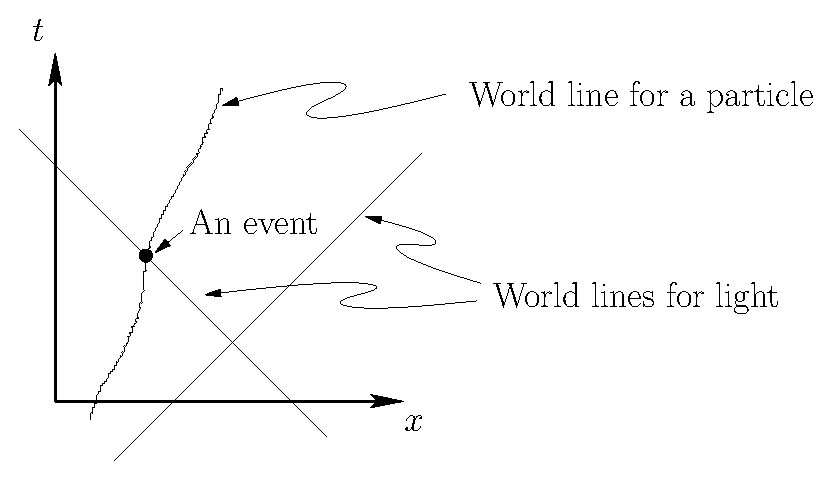
\includegraphics[width=3.5in]{relativistic_spacetime/spacetime1.eps}
\end{center}
\caption{A spacetime diagram with three world lines.  The two world lines for 
light have slopes $+1$ and $-1$.}
\label{fig:spacetime-example}
\end{figure}

Let's use a spacetime diagram to display the world lines of the
three-clock thought experiment of Ch.~\ref{chapter:relativityI},
Section~\ref{section:time-dilation} (see Fig.~\ref{fig:light-clocks}
from that section and Fig.~\ref{fig:worldlines1} in this section).
For example, put clock A at rest at $x = 0$ and clock B at rest at $x
= 0.60\units{lt-s}$.  The world lines for the stationary clocks A
and B are then vertical lines at $x = 0\units{lt-s}$ and $x =
0.60\units{lt-s}$.  Let clock C travel with speed $0.60c$ in the
positive $x$-direction.  Because $c = 1\units{lt-s/s}$, clock C
passes through $x = 0$ at time $t = 0\units{s}$, and it passes
through $x = 0.60\units{lt-s}$ at time $t = 1.0\units{s}$.  It has 
traveled a distance of $0.60\units{lt-s}$ in a time $1.0\units{s}$.
    
Notice in Fig.~\ref{fig:worldlines1} that we have labeled the world
line of clock C as the $t^\prime$ axis.  This is a general result: the
world line of a particular observer (say, someone traveling in a space
ship) is the $t^\prime$ axis for that observer.  This can be
understood by considering a person on a spaceship holding a ball. The
world line for the ball is the same as the world line of the ship and
person since they are all moving together.  From the perspective of
the astronaut, the ball remains right in front of him and isn't moving
anywhere, so it makes sense that that astronaut will say that the
location of the ball remains at $x^\prime = 0$.  And just as it is
true that the points where $x = 0$ in the unprimed frame define the
$t$-axis, so it is that the points where $x^\prime = 0$ in the primed
frame define the $t^\prime$-axis.
    
\begin{figure}[tbp]
\begin{center}
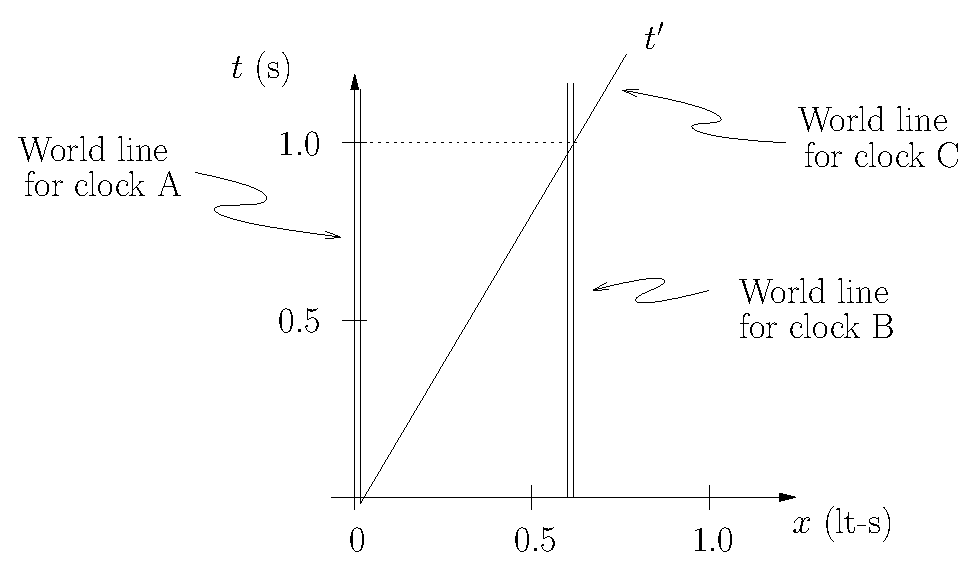
\includegraphics[width=4in]{relativistic_spacetime/worldlines1.eps}
\end{center}
\caption{World lines for the three clocks in the thought experiment
of Section~\ref{section:worldlines}}
\label{fig:worldlines1}
\end{figure}

Some comments are in order:
\begin{enumerate}
\item A world line is nothing more than a plot of time versus
position.  If you ever find yourself stumped about how to plot a
world-line, ask yourself: ``Where is the (whatever) at time $t=0$
(i.e., what is its initial $x$-coordinate)?  Where is it at time 
$t=1$?  At time $t=2$?  \dots''  Then simply plot those points 
and connect them.
\item The slope of a world line is simply $1/v$.  This comes from the
  standard relation: distance = speed $\times$ time, or equivalently, 
  $\Delta x= v \Delta t$.   So $\Delta t =
  \frac{1}{v}\Delta x$.  Practically, this means that if you have a ship
  moving at a speed of, say, $0.5c$, then the slope will be $1/ v$ or
  $2.0\units{s/lt-s}$.  When plotting a world line, this means that
  you go up 2 and over 1 (or over 0.5 and up 1).
\item Don't {\bf ever} forget --- nothing can travel faster than
light, so there should {\bf never} be a world line on a spacetime diagram
 with a
slope whose magnitude is less than 1.  
\item Remember: events are plotted as dots.
\item Label everything clearly.
\end{enumerate}

\begin{figure}[tbp]
\begin{center}
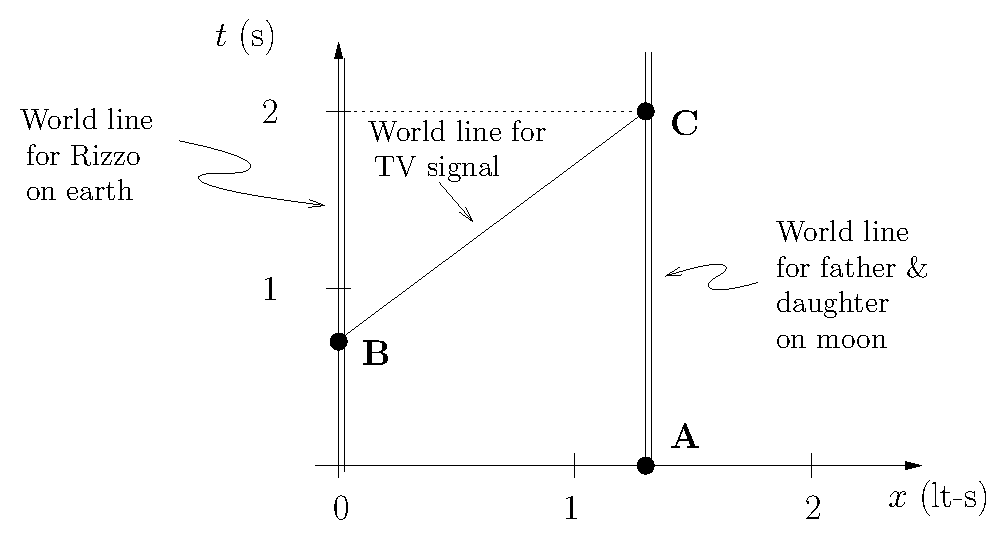
\includegraphics[width=4.2in]{relativistic_spacetime/worldlines2.eps}
\caption{Spacetime diagram for situation discussed in
  Examples~\ref{example:causality-intervals} and
  \ref{example:causality-intervals-diagram}}
\end{center}
\end{figure}

\begin{example}{Spacetime diagram corresponding to 
Example~\ref{example:causality-intervals}} Draw the spacetime diagram
  for the baseball scenario (Cubs losing the World Series) discussed
  in Example \ref{example:causality-intervals}, using the reference
  frame of the Earth/Moon.  Show the world lines for Anthony Rizzo, Jr.,
  the girl and her father, and the TV signal.  Also, show and label
  the following events: A --- girl sneezes, B --- Rizzo strikes out, and
  C --- girl and father see Rizzo striking out.  \solution The world
  lines for Rizzo and the girl/father are simply straight vertical lines
  since they aren't moving in the Earth-Moon reference frame.  If this
  isn't clear, then answer these questions: If we put the Earth at $x
  = 0$ at time $t = 0$, where is the Earth at time $t=1\units{s}$?
  Answer: still at $x = 0$.  At $t=2\units{s}$?  Answer: still at $x =
  0$.  The Earth's world line is nothing more that a set of points
  where $x$ is always zero.  As for the girl/father on the Moon, we
  already said in Example \ref{example:causality-intervals} that they
  are about $1.3\units{lt-s}$ away from the Earth.

We know from the problem that the girl/father see the strikeout
$2\units{s}$ after she sneezes.  So, if she sneezes at $t = 0$ (it is
arbitrary as to what we choose as the $t = 0$ time), then the TV
signal arrives at $t = 2\units{s}$.  It must have been sent from the
Earth at an earlier time, and since it travels at the speed of light,
then the world line for the TV signal is a $45^\circ$ line.  The only
thing left is to plot the three dots for the events.

Note that if you imagine a line between A and B, that line would 
have a slope with magnitude less than 1 (i.e., too shallow), 
indicating that nothing can travel between these two events, 
consistent with the result in Example 1 that the interval is space-like 
and the corresponding events can't be causally linked.
\label{example:causality-intervals-diagram}
\end{example}


\section[the relativity of simultaneity]{Ordering of events --- the 
relativity of simultaneity}

Every event has a set of space and time coordinates.  In Example
\ref{example:causality-intervals-diagram} above, we would say that the
event A (girl sneezes) occurs at time $t=0$ and location $x =
1.3\units{lt-s}$.  Similarly, we can determine the location and times
of events B and C, all as measured by observers in the Earth-Moon
reference frame. Let's add one more event to the scenario: let's say
that at time $t=0$, the pitcher Masahiro Tanaka, Jr., pitches the ball
toward Castro.  In Fig.~\ref{fig:father-daughter} we have added this event and
labeled it P.  In the Earth-Moon frame, we can say quite definitively
that A and P are simultaneous and come first, then B, then C.  Also, A
and C happen at the same location, and P and B happen at the same
location.

\begin{figure}[tbp]
\begin{center}
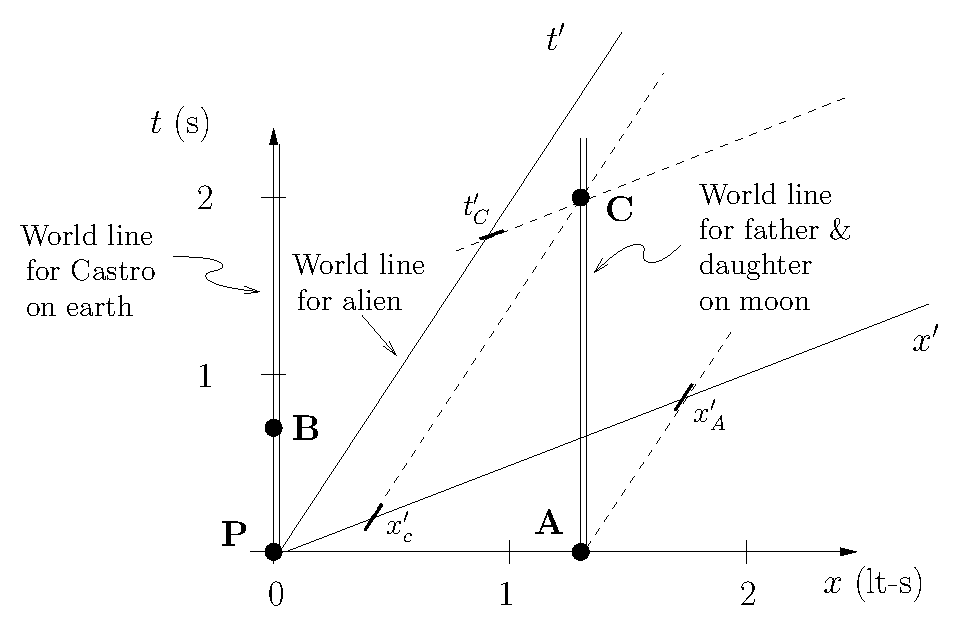
\includegraphics[width=4.3in]{relativistic_spacetime/worldlines3.eps}
\end{center}
\caption{Extension of spacetime diagram in Example
\ref{example:causality-intervals-diagram}.}
\label{fig:father-daughter}
\end{figure}
    
Special relativity helps us answer the following question: how does an
observer moving in a different reference frame view these same events?  We
won't worry here about the actual numerical values of $x^\prime$ and
$t^\prime$ (the position and time as measured by a different observer), but
we can say quite a lot about the ordering of events in space and time
by looking at the spacetime diagrams.


We have added another world line to Fig.~\ref{fig:father-daughter},
namely, the world line for a hypothetical alien whizzing past the
Earth just as the pitch is thrown.  This alien is monitoring the game
to try to understand human culture.  We assume the alien is traveling
at a speed $0.5c$; hence, the world line has a slope of 2.

We have already commented that the world line of an observer in a
primed frame is simply the $t^\prime$ axis for that frame, so we have
labeled the alien's world line $t^\prime$. But where should we put the
$x^\prime$-axis and what scale should we put on it?  It turns out that to
satisfy the invariance of the speed of light, we must draw the
$x^\prime$-axis at the same angle relative to the $x$-axis as the angle of
the $t^\prime$-axis relative to the $t$-axis. This means the slope of the
$x^\prime$-axis is equal to the speed $v$ of the primed frame relative to the
unprimed frame.
    
Recall that the $t^\prime$-axis represents points where $x^\prime =
0$.  It turns out that $x^\prime$ is constant along any line parallel
to the $t^\prime$-axis.  In other words, lines parallel to the $t^\prime$-axis
are equal-location lines for the primed frame of reference, just as
the $t$-axis and all lines parallel to it are each lines of equal
location for the unprimed frame of reference.  The same ideas work for
events on lines parallel to the $x$ or $x^\prime$ axes; events on a line
parallel to the $x$-axis are simultaneous in the unprimed frame, and
events on a line parallel to the $x^\prime$-axis are simultaneous in the
primed reference frame.
    
We can use these ideas to ``read off'' coordinates for events in
both reference frames.  As an example, let's look at event C in
Fig.~\ref{fig:father-daughter}.  We have already commented that in the
unprimed frame, its $x$ location is $1.3\units{lt-s}$ and its time
is $2\units{s}$.  The coordinates of this event in the alien's
reference frame are determined by drawing lines parallel to the
$x^\prime$ and $t^\prime$ axes (shown as dotted lines in
Fig.~\ref{fig:father-daughter}).  The intersections of these
construction lines with the opposing primed axis gives the $x_C$ and
$t_C$ coordinates. The rules for determining coordinates can be
summarized as follows:
\begin{enumerate}
\item To find $x_C$, draw a straight line through C parallel to the
$t$-axis and read off where it crosses the $x$-axis.  
\item To find $t_C$ draw a straight line through C parallel to the
$x$-axis and read off where it crosses the $t$-axis.  
\item To find $x_C^\prime$, draw a straight line through C parallel to
the $t^\prime$-axis and read off where it crosses the $x^\prime$-axis.
\item To find $t_C^\prime$, draw a straight line through C parallel to the
$x^\prime$-axis and read off where it crosses the $t^\prime$-axis.
\end{enumerate}

Using this type of construction, we can see that although events A and
C occur at the same place in the unprimed (Earth-Moon) reference
frame, event C happens to the left of the event A in the primed
(alien) reference frame.  This is easy to understand: the alien is far
from the Moon when event A happens, so A is far ``to the right,''
whereas the alien is close to the Moon when event C happens, so from
the alien's perspective, C isn't so far to the right, i.e.,
smaller $x^\prime$ coordinate.
    
    But what about the ordering of events in time?  We have commented
that the invariance of the spacetime interval says that if two
observers disagree about distances, then they will have to disagree
about time intervals as well.
    
\begin{boxittext}
{{\bf In preparation for class:} Look at the $t^\prime$ coordinates for events
P and A.  In the Earth-Moon reference frame, these events are simultaneous.
What about in the alien reference frame?
}
\end{boxittext}

We have said that any two events on a line parallel to the
$x^\prime$-axis are simultaneous in the primed frame of reference.
Similarly two events that lie on a line parallel to the $x$-axis are
simultaneous in the unprimed frame.  However two different events
cannot lie both on a line parallel to the $x$-axis and parallel to the
$x^\prime$-axis.  Thus two events that are simultaneous in one frame cannot
be simultaneous in the other frame.  We explore this idea in the
following example.

\begin{example}{Simultaneity is Relative}  
Einstein showed, with the following thought experiment, that two events
which occur at the same time but at different places in one frame,
occur at different times in another frame.

\begin{figure}[tbp]
\begin{center}
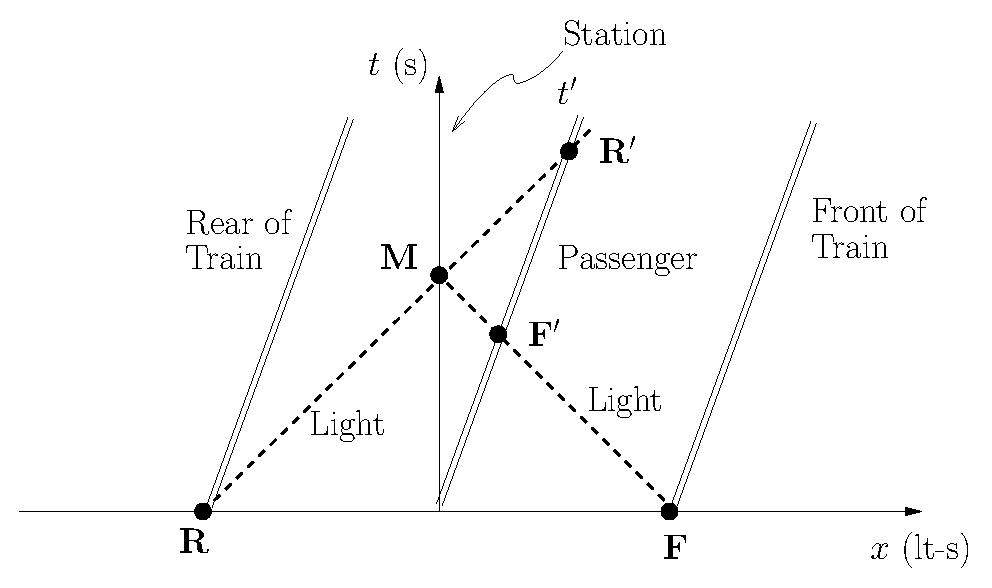
\includegraphics[width=4.2in]{relativistic_spacetime/worldlines4.eps}
\end{center}
\caption{Spacetime diagram for train of Example 
\ref{example:simultaneity}. (Light
world lines shown as dashed lines.)}
\label{fig:simultaneity}
\end{figure}

Imagine a train moving past a station.  By chance, lightning
happens to strike the front and back of the train at the same time
according to observers on the station platform.  Light pulses from
these strikes travel toward the middle of the train, where a passenger
observes their times of arrival.  Do the light pulses arrive
simultaneously or does one arrive before the other, and if so, which
one?
\solution
Use a spacetime diagram, Fig.~\ref{fig:simultaneity}, with the
station at rest in the unprimed frame and the train at rest in the
primed frame.  The $x$- and $x^\prime$-axes both lie along the track.
(Note:  this does {\bf not} mean that the $x$- and $x^\prime$-axes
are the same thing on a spacetime plot.  The $x^\prime$-axis is not
shown in Fig.~\ref{fig:simultaneity}, but remember that it is the mirror
image of the $t^\prime$-axis about a $45^\circ$ line; i.e., the angle
between the $t$- and $t^\prime$-axes is the same as the angle between
the $x$- and $x^\prime$-axes.)
The world line for the middle of the station is shown as the $t$-axis.

Because all parts of the train are at rest in the primed frame, we
draw the world lines for the front and the rear ends of the train
parallel to the $t^\prime$-axis.  Also, in
Fig.~\ref{fig:simultaneity}, we have chosen the world line for the
passenger riding in the exact middle of the train to be the
$t^\prime$-axis.  In the primed frame the front and rear world lines
are then equidistant from the passenger, by definition.

The lightning strikes occur at points R and F on the world lines of 
the rear and front of the train.  Because each strike represents an 
event and because these two events occur simultaneously in the 
station frame, R and F must be drawn on the same horizontal line.  
We arbitrarily choose this line to be at $t = 0$.

The light pulses produced by the lightning strikes travel with speed
$c = 1\units{lt-whatever per whatever}$ from the event F back toward
the passenger and from R forward toward the passenger.  The pulse from
F is represented by a world line of slope $-1$ and the pulse from R is
represented by a world line of slope $+1$.  Figure
\ref{fig:simultaneity} shows that the pulse from F arrives at the
passenger's world line (at F$^\prime$) earlier (i.e., at a smaller
value of $t^\prime$) than does the pulse from R, which arrives at
R$^\prime$.

The passenger must conclude that the front strike occurred before 
the rear strike because she is sitting in the middle of the train, 
equidistant from R and F, and she knows the light pulses must have 
taken the same time (in her frame) to reach her.  By the same 
argument, an observer on the station platform who was at the exact 
middle of the train at $t = 0$ when the strikes occurred, sees the 
pulses at the same time.  This is shown on the spacetime diagram 
by the fact that the world lines of the pulses cross the world line of 
the middle of the station at $x = 0$ (event M) at the same time.
\label{example:simultaneity}
\end{example}

\newpage

\section*{Problems}
\markright{PROBLEMS}

\begin{problem}
If two events are separated by a time-like interval in one
frame of reference, are they separated by a time-like interval in all
frames of reference?  Explain.
\end{problem}

\begin{problem}
A simple way of synchronizing two clocks at rest relative to one
another is to stand exactly halfway between them and emit light pulses
toward each of them at the same instant of time.  Each clock is then
set to 0 when the synchronizing pulse reaches it.
  \begin{enumerate}
  \item How does this scheme ensure that the clocks are started
    simultaneously?  
  \item On a spacetime diagram show the world lines of two
    clocks at rest in the unprimed frame of reference at $x = 0$ and at $x =
    L$, along with the world lines of two synchronizing light pulses that
    start from the midpoint and reach each of the two clocks at $t = 0.$
  \end{enumerate}
\label{prob:synchronizeB}
\end{problem}

\begin{problem}
  Events A, B, and C are shown on the spacetime diagram in
  Fig.~\ref{fig:spacetimeI}.
  \begin{figure}[h]
  \begin{center}
    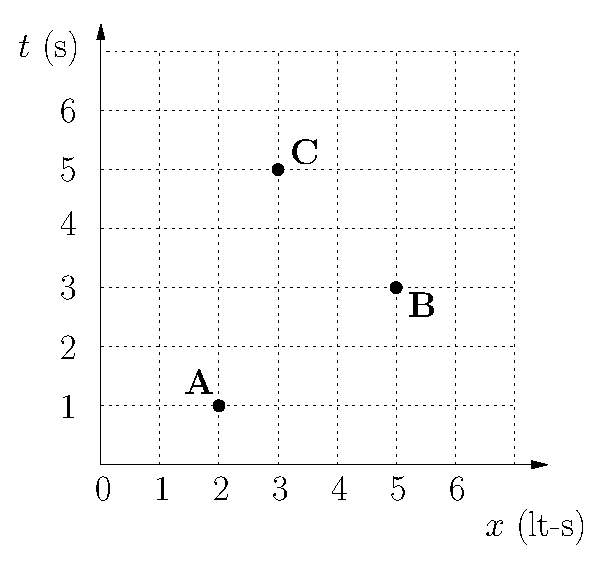
\includegraphics[width=2.8in]{relativistic_spacetime/p_spacetimeI.eps}
  \caption{Figure for Problem \ref{prob:spacetimeI}.}
  \label{fig:spacetimeI}
  \end{center}
  \end{figure}
  \begin{enumerate}
  \item Calculate the value of the squared interval for each pair of
    events, i.e., find $I^2_{AB}$, $I^2_{AC}$, and $I^2_{BC}$.  
  \item Label each interval as time-like, space-like, or light-like.  
  \item In the frame shown, event A occurs before B, which occurs before
    C.  Which pairs of events could have their time-order reversed
    (switching before and after) by choosing an appropriate reference
    frame?  
  \item In the frame shown, event B occurs to the right of C, which
    occurs to the right of A.  Which pairs of events could have their
    space-order reversed (switching left and right) by choosing an
    appropriate reference frame?  
  \item Which events could be a ``cause'' for which other events?
  \end{enumerate}
\label{prob:spacetimeI}
\end{problem}

\begin{problem}
Fig.~\ref{fig:spacetimeII} shows a spacetime diagram with seven straight lines
through the origin labeled with capital letters A through G.  Various
events are marked as points with small letters a through e.  The $x$-$t$
axes belong to the Earth's reference frame.

\begin{figure}[htbp]
\begin{center}
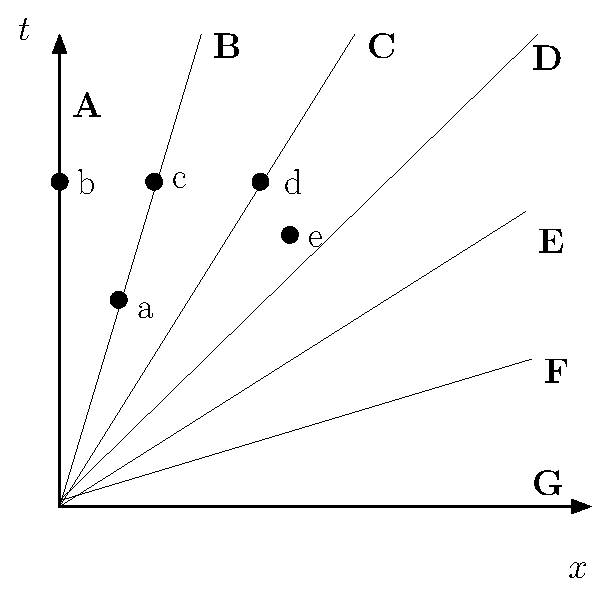
\includegraphics[width=2.5in]{relativistic_spacetime/p_spacetimeII}
\caption{Figure for Problem \ref{prob:spacetimeII}.}
\label{fig:spacetimeII}
\end{center}
\end{figure}
 
\begin{enumerate}
\item Which line is a world line of an object at rest relative to the Earth?
\item Which line is a world line of a spaceship traveling at speed  
$+0.3c$ relative to the Earth?
\item Which line is a world line of a light pulse emitted by the
spaceship as it passes the Earth? 
\item Which events happen simultaneously in the Earth frame?  
\item  Which events happen simultaneously in the spaceship frame?  
\item Which pairs of events are clearly separated by space-like
intervals?  Which are clearly separated by time-like intervals?
\end{enumerate}
\label{prob:spacetimeII}
\end{problem}

\begin{problem}
For Example \ref{example:simultaneity} in the text, show from
the spacetime diagram in Fig.~\ref{fig:simultaneity} that lightning
hit the front of the train at a negative value of $t^\prime$, but that
lightning hit the rear of the train at a positive value of $t^\prime$.
Use the rule for finding the $t^\prime$ coordinate of an event to
solve this problem.  [Hint: you might want to extend some of the axes
in the negative direction.]  
\end{problem}

\begin{problem}
Farmer Brown, at rest in his frame, carries a ladder through
a barn.  According to Farmer Brown, the ladder measures
$20\units{lt-ns}$.  According to observers at rest with respect
to the barn, Farmer Brown and his ladder are moving at a
speed $0.80c$ (alternately, Farmer Brown sees the barn 
moving at speed $0.80c$).  In the barn's frame, the
front door of the barn is at $x = 0 \units{lt-ns}$ and the back 
door is at $x = 16\units{lt-ns}$.
\begin{enumerate}
\item Calculate the length of the ladder as measured by
observers in the barn's reference frame.  According to
these observers, will the ladder fit within the barn?
\item Calculate the length of the barn as measured by
Farmer Brown.  According to Farmer Brown, will the ladder
fit within the barn?
\item Draw a careful spacetime plot for this situation,
with appropriate tick marks on the axes (labeled with
numbers).  Starting with the barn frame, draw world
lines for the entrance and exit of the barn (i.e., the
front and back doors).  Draw also world lines for the front and
back of the ladder (which is moving as viewed in the
barn frame).  The distance between the front and back of
the ladder in your plot should agree with your answer
to part (a), and the slopes of these lines should be
consistent with the known velocities.
\item Label the following events on your diagram:
A = front of ladder enters the barn; B = front of ladder
leaves the barn; C = back of ladder enters barn;
D = back of ladder leaves barn.  Determine the order
of these events in time as viewed from the barn's
reference frame.  Is this result consistent with your
answer to (a), i.e., whether or not the ladder fits in the
barn, according to barn-frame observers?  (Consider
whether the back of the ladder enters the barn before
or after the front of the ladder leaves the barn.)
\item Determine the order of events A, B, C and D as
viewed from Farmer Brown's reference frame.  Is this
result consistent with your answers to (b)?
\item Based on your answers for this problem, can you
see how relativistic time-ordering (i.e, the fact that
different observers do not necessarily agree on the
ordering of events in time) is necessarily linked with
length contraction?
\end{enumerate}
\label{prob:farmer}
\end{problem}

\newpage
\begin{figure}[!h]
\[ \includegraphics[width=5.5in]{relativistic_spacetime/p_solar_flare.eps} \]
\caption{Figure for Problem \ref{prob:solar_flare}.}
\end{figure}

\newpage

\begin{problem}
The Earth is $8\units{lt-min}$ from the Sun.  An astronomer on Earth,
looking through a telescope, notices the sudden appearance of a giant
solar flare on the Sun's surface.  At precisely that instant (when the
astronomer detects the flare), a Klingon space ship whizzes over his
head at speed $0.8c$, heading straight for the Sun.
\begin{enumerate}
\item On the facing page, construct a spacetime diagram for this situation.  
  Label the following three events: {\bf A}: Klingon ship hits Sun, 
  {\bf B}:  flare occurs on Sun, and {\bf C}: Klingon ship passes Earth.  
  (Note that event B is the occurrence of the flare {\em on\/} the Sun, 
  not the detection of the flare by an astronomer on Earth.)
\item Order the events A, B, C, from earliest to latest, according to
  Earth-based observers.
\item Calculate the time intervals $\Delta t$ between each pair of
  events (AB, AC, and BC), according to Earth observers.
\item Calculate the interval $\Delta t^\prime_{BA}$ between events B
  and A, but now according to Klingon ship observers.
\item Classify each of the intervals as space-like, time-like or
  light-like.
\end{enumerate}
\label{prob:solar_flare}
\end{problem}

% \begin{problem}
% A cosmic ray particle moving down toward Earth at speed $0.99c$ decays
% $2.0\units{$\mu$s}$ after it was produced as measured in the frame in
% which the particle is at rest.
% \begin{enumerate}
% \item Represent the birth and decay of the particle on a spacetime
%   diagram.
% \item In the cosmic ray's rest frame the Earth is moving toward it.
%   In this frame, how far, in light-$\mu$s, did the Earth travel during
%   the particle's lifetime?
% \item Observers in the Earth's frame see the particle coming down
%   toward Earth.  How long did the particle live according to these
%  observers and how far did it travel?
% \end{enumerate}
% \label{prob:cosmic_ray}
% \end{problem}

\begin{problem}
Two spacecraft, {\em Aaaak} and {\em Blech}, are carrying aliens from 
the planet Zortox to Earth.  Both spacecraft are traveling
at a speed of $0.6c$ relative to the Earth, with {\em Aaaak} in
front.  In the Earth's frame, {\em Aaaak} and {\em Blech} are
a distance $8.0\units{lt-s}$ apart. 
At the moment that {\em Aaaak} passes Earth, the Zortoxians aboard {\em Aaaak} 
dump its garbage.  At a time $10.0\units{s}$ later 
(as measured by earthlings) {\em Blech} dumps its garbage.  
\begin{enumerate}
\item Draw a spacetime diagram in Earth's frame that includes 
worldlines for Earth, {\em Aaaak}, and {\em Blech}.  Indicate and label 
the events corresponding to the garbage dumps.
\item How far has {\em Blech} traveled during the $10.0\units{s}$ 
between the two garbage dumps measured by earthlings?
\item What is the distance between the two garbage dump events measured by 
earthlings?
\item What is the distance between the two garbage dump events 
measured by the Zortoxians on board their ship?
\item Calculate the time interval between garbage dump events measured by 
the Zortoxians on board their ship.
\end{enumerate}
\label{prob:two_ships}
\end{problem}

%\begin{problem}
%Two spacecraft ({\em Aaaak} and {\em Blech}) carrying aliens from 
%the planet Zortox are traveling toward  Earth (with {\em Aaaak} in front) 
%at a speed of $0.6c$ relative to the Earth.  In the Earth's frame of 
%reference {\em Aaaak} and {\em Blech} are $8.0\units{lt-s}$ apart. 
%At the moment they pass Earth, the Zortoxians aboard {\em Aaaak} 
%dump its garbage, and $10.0\units{s}$ later 
%(as measured by earthlings) {\em Blech} dumps its garbage.  
%\begin{enumerate}
%\item Draw a spacetime diagram in Earth's frame that includes 
%worldlines for Earth, {\em Aaaak}, and {\em Blech}.  Indicate and label 
%the events corresponding to the garbage dumps.
%\item How far has {\em Blech} traveled during the $10.0\units{s}$ 
%between the two garbage dumps measured by earthlings?
%\item What is the distance between the two garbage dump events measured by 
%earthlings?
%\item What is the distance between the two garbage dump events 
%measured by the Zortoxians on board their ship?
%\item Calculate the time interval between garbage dump events measured by 
%the Zortoxians on board their ship.
%\end{enumerate}
%\label{prob:two_ships}
%\end{problem}


\newpage

\begin{problem}
A train of rest length $40\units{lt-ns}$ moves along the
tracks at $0.8c$ and is struck by two lightning bolts.  One bolt hits
the front of the train and the other hits the back.  According to
observers  on the tracks the bolts are simultaneous.
\begin{enumerate}
\item How far apart did the lightning bolts strike according to 
observers on the tracks?  
\item According to riders on the train, how much time passed between the
striking of the lightning bolts?  
\item According to riders on the train, which lightning bolt 
struck first? 
\end{enumerate}
\end{problem}

\begin{problem}
Joe holds and lights a sparkler, and one minute later, it goes
out.  Cheri, riding in a rocket past these events, notes that, as
measured in her frame, the sparkler burned for 100 seconds.
\begin{enumerate}
\item How far apart in Cheri's frame did these two events (lighting
and going out) occur? 
\item As measured by Cheri, how far did the lit sparkler travel, and
how fast was it moving?  
\item As measured by Joe, how fast was Cheri traveling during the one
minute of sparkler light, and how far did she travel?
\end{enumerate}
\label{prob:sparkler}
\end{problem}

\newpage

\begin{problem}
The spacetime diagram in the figure shows the world lines of the Earth,
a star, and a rocket, as well as several labeled events.
\begin{figure}[!h]
\begin{center}
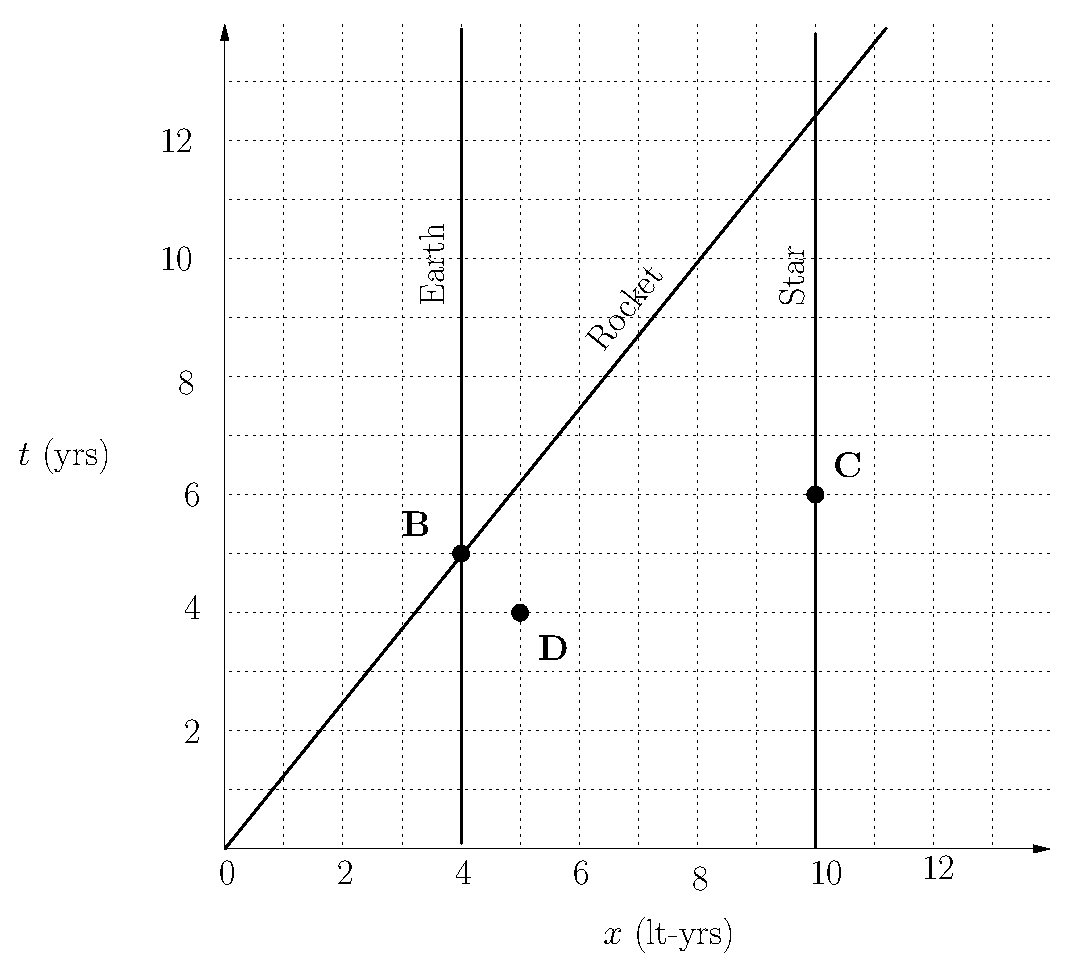
\includegraphics[width=3.68in]{relativistic_spacetime/p_spacetimeIII.eps}
\end{center}
\caption{Figure for Problem \ref{prob:spacetimeIII}.}
\end{figure} 
\begin{enumerate}
\item On the diagram, label as ``A'' the event ``Rocket arrives
at Star.''
\item Determine the speed of the Rocket, as measured by Earth
observers.
\item Determine the time between passing the Earth and passing the
Star, as measured by Rocket observers.
\item Determine the distance between the Earth and the Star, as
measured by Rocket observers.
\item Draw the world line of a lost satellite passing the Earth at the
same time as the Rocket, but going away from the Star at a speed that
is $\frac{1}{2}$ of the Rocket speed (as determined by Earth
observers.)  Label this line ``Satellite.''
%\item Determine the speed of the satellite as measured by Rocket observers.
%This part removed in 2011 when velocity transformations moved to mom/energy
%chapter.
\item Order the events A, B, C, D, from earliest to latest, as
observed in the Earth-Star reference frame.
\item Order the events A, B, C, D, from earliest to latest, as
observed in the Rocket reference frame.  
\item In some reference frame, the events C and D are simultaneous.
In that frame, what is the distance between events C and D?
\item Explain why no one could ever measure the proper time between
events C and D.  
\end{enumerate}
\label{prob:spacetimeIII}
\end{problem}


\input{relativistic_momentum_and_energy/relativistic_momentum_and_energy}

\chapter[Applications of the Conservation Laws]{Applications of the 
Relativistic Conservation Laws}
\label{chapter:relativity_app}

%\section*{Objectives}
%\begin{objectives}
%\item Describe increases and decreases in mass associated with processes
%that release or absorb kinetic energy.
%\item Apply the relativistic conservation laws to ``explosions,'' in
%which one particle decays into two particles, including cases in
%which one or both outgoing particles have zero rest mass.  
%\item Do the same for simple collisions with all particles traveling
%along a line.
%\item Be able to describe the processes of nuclear fusion and fission,
%and explain how these processes result in kinetic energy production.  
%\item Given information about nuclear masses, calculate the amount of
%kinetic energy gained in a fusion or fission process.
%\end{objectives}

\section{Introduction}

You should now understand why Einstein's postulates
require new definitions of momentum and energy.  The classical
momentum is not conserved, nor in general is the total mass of the
particles in an interaction.  In place of these, relativistic momentum
and relativistic energy are conserved, and they are conserved in any
inertial frame.  

In this chapter, we apply these new, relativistic conservation laws to 
analyze collisions and decays of subatomic
particles.  The key result in these applications is the ability for
matter to be converted into kinetic energy and vice-versa.  In relativistic
collisions, the amount of matter that you start with is not the same
as the amount of matter that you finish with!  We also discuss the
principles behind nuclear fission and nuclear fusion.

\section{Changes of Rest Energy}
  Much of the light you see comes from changes in rest energy of
atoms.  Examples are sunlight, light from a candle flame, a lightning
flash, light emitted by a fluorescent lamp, light from the phosphor
coating on the screen of a television set or a video monitor, and
laser light.  In all these examples, the basic mechanism is that an
atom in an ``excited'' state releases its energy in the form of a
photon, with the atom going into its ground (lowest possible) state,
or into an excited state of lower energy.  We can represent the
emission process by the simple reaction equation

\begin{equation}
{\bf A}^\ast \rightarrow {\bf A} + \gamma. 
\label{eq:photon_emission}
\end{equation}
Here ${\bf A}^\ast$ represents the excited atom, ${\bf A}$ the atom in its
ground or lowest state, and $\gamma$ (Greek {\em gamma}) the photon.

\begin{figure}[tbp]
\begin{center}
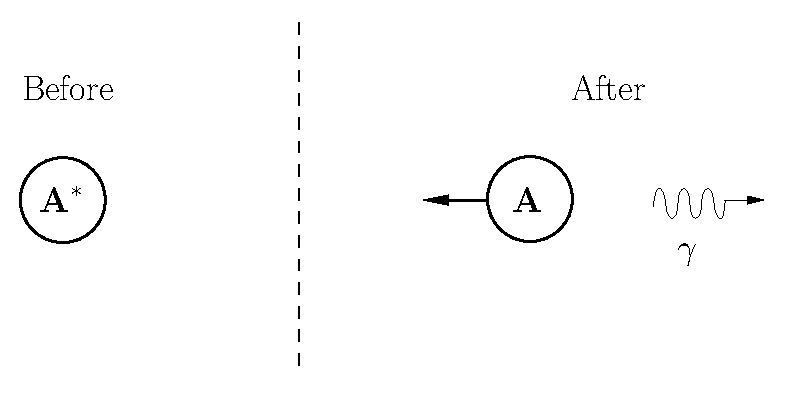
\includegraphics[width=3.5in]{relativity_conservation/photon_emission1.eps}
\end{center}
\caption{An excited atom emits a photon and recoils.}
\label{fig:photon_emission1}
\end{figure}

In Fig.~\ref{fig:photon_emission1}, the excited atom is shown at rest,
so all of its energy is rest energy and it has no momentum.  But the
photon has energy, and from the relation $E = pc$, it also has
momentum.  And because momentum must be conserved, the atom recoils.
We can write the conservation of energy equation for the reaction in
Eq.~(\ref{eq:photon_emission}) as follows
\begin{equation}
\text{Rest Energy of ${\bf A}^\ast$} = \text{Energy of ${\bf A}$} 
+ \text{Energy of photon}.
\end{equation}
     
Because both the kinetic energy of ${\bf A}$ and the photon energy are
positive numbers, the rest energy (i.e., the mass) of the
excited-state atom must be greater than that of the ground-state atom.
Therefore, in the emission process rest energy, i.e., mass, is
converted to kinetic energy.
     
When light is absorbed by an atom, exactly the opposite effect occurs.
The atom begins in its ground state, absorbs the photon energy and
goes into an excited state.  Again, by conservation of energy, the
excited atom must have more rest energy than the ground-state atom.

Another everyday example of changing rest energy occurs in chemical
reactions.  For example, the reaction for the oxidation of a carbon
atom
\begin{equation}
\text{C} + \text{O}_2 \rightarrow \text{CO}_2
\end{equation}
is known to release energy in the form of one or more photons.
Therefore the sum of the masses of C and O$_2$ must be greater than
the mass of the carbon dioxide molecule.  The change in rest energy in
the case of chemical reactions is typically on the order of
$1\units{eV}$ (or $1.6\times 10^{-19}\units{J}$).  Much larger
energies, on the order of $1\units{MeV}$, are involved in nuclear
reactions.  An example of a nuclear reaction is the decay of a neutron
into a proton, an electron, and an electron antineutrino:
\begin{equation}
n \rightarrow p + e^- + \bar{\nu}_e.
\end{equation}
Here the excess mass of the neutron over the mass of the proton plus
electron (the electron antineutrino has very small mass) is converted
to the kinetic energy of the three reaction products.

Another important example of changes in rest mass is the production of
new particles in a high energy particle accelerators.  In these
accelerators high-speed particles are shot at target particles and
some of the kinetic energy of the incoming particles is converted to
rest energy.  In this way hundreds of new particles, most with
lifetimes between $10^{-10}$ and $10^{-23}\units{s}$, have been
produced.  You'll learn more about these new particles next semester
in PHYS 212.

\section[General Strategy]{General Strategy for 
Applying the Relativistic Conservation Laws}


 In a typical problem you are given information about the particles
before an interaction and asked to compute certain properties of the
outgoing particles after the interaction.  You do this by writing down
equations that express the fact that the sum of the incoming momenta
is equal to the sum of the outgoing momenta and the sum of the
incoming energies is equal to the sum of the outgoing energies.  What
quantities should be used in writing these equations?  Here is some
time-saving advice.
\begin{quote}
Always write the conservation of momentum and conservation of energy
equations in terms of momentum and energy or mass variables, never in
terms of velocity or kinetic energy.
\end{quote}

This rule keeps the algebra as simple as possible --- it gets around
having to solve simultaneous equations with the $\sqrt{1-v^2/c^2}$
terms that can make the algebra messy.  For example, if you are given
the velocity of one or more particles in the problem statement, first
calculate the momentum and energy of each particle from the given
velocities.

A second piece of advice:
\begin{quote}
When working with ``eV'' units (e.g., MeV for energy, MeV/$c$ for
momentum, MeV/$c^2$ for mass), don't ever put any numbers in for the
speed of light $c$.  Just leave it as ~``$c$.''  The units will then
automatically take care of themselves.
\end{quote}

For example, if you have an motionless electron, its energy can be
obtained from $E^2 = p^2c^2+m^2c^4$. For a motionless electron  $p = 0$, 
so $E= mc^2 = 0.511\units{MeV/$c^2$}\times c^2 = 0.511\units{MeV}$.  
(See section \ref{section:rel-units}.)

\begin{example}{Emission of a photon by a nucleus.}
\label{ex:nuclear_decay}
An excited atomic
nucleus, of mass $5.00\units{GeV/$c^2$}$ and at rest, as in
Fig.~\ref{fig:photon_emission2}, decays to its ground state by
emitting a photon of energy $2.00\units{GeV}$.  Calculate the recoil
velocity and mass of the ground-state nucleus.
\solution
First draw a picture, and label each particle with its value of
energy and momentum.  Before the decay the excited nucleus has zero
momentum because it is at rest.  And from $E^2 = p^2c^2 + m^2c^4$, with 
$p =0$, we know its energy is the same as its rest energy, namely 
$5.00\units{GeV}$.

\begin{figure}[tbp]
\begin{center}
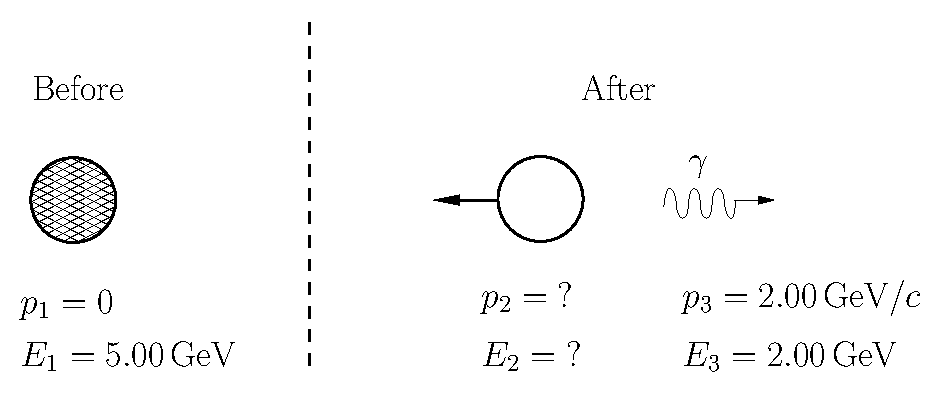
\includegraphics[width=4in]{relativity_conservation/photon_emission2.eps}
\end{center}
\caption{Emission of a photon by a nucleus as discussed in Example 
\ref{ex:nuclear_decay}.}
\label{fig:photon_emission2}
\end{figure}

After the decay the ground-state nucleus recoils with unknown energy
and momentum, $E_2$ and $p_2$.  Also, the emitted photon has an energy
of $2.00\units{GeV}$, as specified in the problem.  And because the
photon's mass is zero its momentum has the same numerical value as its
energy.  Notice that in the diagram there are two unknowns, the
energy and momentum of the recoiling ground-state nucleus.  We plan to
solve for these two unknowns with two equations, the energy and
momentum conservation equations.
     
Looking at the diagram, we write down the energy conservation equation
in terms of the symbols and numerical quantities shown in the
diagram:
\[ 5.00\units{GeV} = E_2 + 2.00\units{GeV}. \]
Similarly, we write the momentum conservation equation in terms of
symbols and numerical quantities shown in the diagram:
\[ 0 = p_2 + 2.00\units{GeV/$c$}.  \] From these conservation-law
equations we easily solve for the energy and momentum of the recoiling
nucleus to obtain $E_2 = 3.00\units{GeV}$ and $p_2 =
-2.00\units{GeV/$c$}$.  Now that we've obtained expressions for the
energy and momentum of the recoiling ground-state nucleus, we can find
its velocity using a formula from Problem
\ref{chapter:relativity_pande}.\ref{prob:rel-u-p-e} (and from Table
\ref{table:rel-defs}):
\[ u_2 = \frac{p_2c^2}{E_2} = \frac{(-2.00\units{GeV/$c$})\times c^2}
           {3.00\units{GeV}} = -\frac{2}{3}, \]
and its mass from 
\begin{eqnarray}
m_2c^2 &=& \sqrt{E_2^2 - p_2c^2} \nonumber \\
       &=& \sqrt{(3.00\units{GeV})^2 - (2.00\units{GeV/$c$})^2 \times
            c^2} \nonumber \\
       &=& \sqrt{5}\units{GeV}, \nonumber 
\end{eqnarray}
so the mass is $m_2 = \sqrt{5}\units{GeV/$c^2$}\simeq 2.24\units{GeV/$c^2$}$.

Notice that even though we were asked to find the velocity and mass
of the recoiling nucleus, we didn't use these variables in our
analysis until the very end, after we solved for its energy and
momentum.
\end{example}

\section[Fusion and fission]{Nuclear masses, fusion and fission}


A particularly important application of the material in this chapter
is nuclear power generation.  There are two main approaches: fusion
and fission.  Nuclear fusion involves the merging (fusing) of two
light nuclei (usually hydrogen) to form a more massive nucleus
(usually helium), whereas fission\footnote{The story of how fission was
discovered is quite interesting. It starts with Lise Meitner and Otto
Hahn, who conducted ``transuranium'' experiments where they bombared 
massive nucleii with the goal of making {\bf more} massive nucleii
(more massive than uranium). But the experiments produced puzzling results.
Meitner -- with her nephew Otto Frisch -- later provided an explanation.
Instead of making more massive nucleii, they realized that the nucleii
were breaking up with a resulting loss of mass, and Meitner used 
Einstein's theory of relativity
to explain the increase in energy observed in the process. Meitner -- who
was inexplicably overlooked for the Nobel Prize for the fission discovery --
also discovered a radiation process which was named the {\em Auger effect}
after a scientist who also discovered this process, a couple of years
{\bf after} Meitner had discovered it.}
 involves the splitting of a very
massive nucleus (e.g., uranium) into two or more lighter nuclei.
For the process to release kinetic energy, conservation of
relativistic energy requires that the end product(s) have a smaller
total mass than the initial nucleus or nuclei.

\begin{figure}[tbp]
\begin{center}
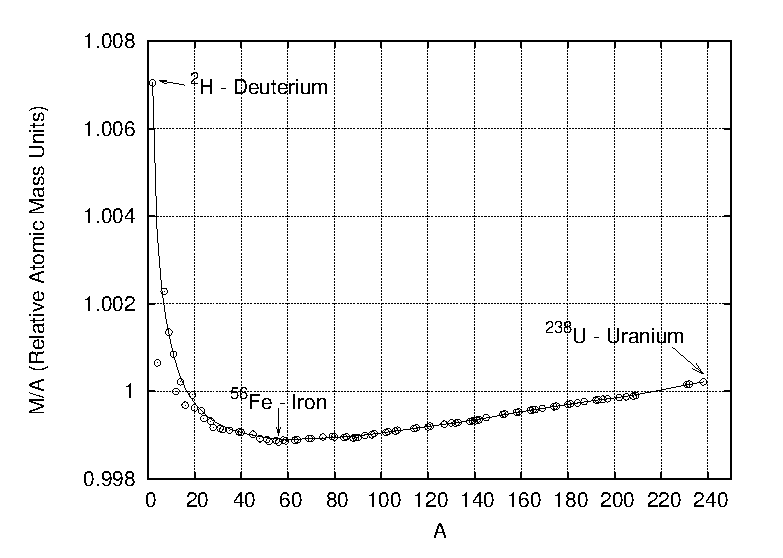
\includegraphics[width=4.5in]{relativity_conservation/mass_per_nucleon.eps}
\end{center}
\caption{Plot of mass per nucleon (proton and neutrons) for the 
elements versus the number of nucleons $A$. (Data from NIST:
http://physics.nist.gov/PhysRefData/Compositions/)}
\label{fig:mass_per_nucleon}
\end{figure}

Figure \ref{fig:mass_per_nucleon} shows a plot of the masses of the
elements, divided by the total number of protons and neutrons
(nucleons) in the nucleus of each atom.  This plot is very
illuminating when considering fusion and fission processes.  
The
fusion of two $^2$H nuclei to form a single $^4$He nucleus results in
a lower overall mass, since the number of nucleons does not change; 
consequently, this process releases kinetic
energy.  On the other hand, elements with large atomic number $A$
have a larger mass/nucleon than those with intermediate values of $A$;
consequently, kinetic energy can also be released by splitting up one of
these heavier atoms (fission).

Of the two processes --- fission and fusion --- fission is a much
easier process to achieve in the laboratory or in industrial
processes.  Many large nuclei are naturally unstable, e.g., $^{235}$U can
spontaneously decay via the fission process ${}^{235}\text{U} \rightarrow
{}^{134}\text{Xe} + {}^{100}\text{Sr} + {}^1n$.  Practically, then, the
issue boils down to setting things up such that the process can be
accelerated when desired, and can be inhibited when unwanted.  From
that perspective, the concept of a chain reaction is relevant.  The
idea of combining multiple nuclear fissions into chain reactions ---which was pioneered
by Lise Meitner, Otto Hahn, Fritz Strassmann, and Enrico Fermi in the
1930s --- is straightforward: if the neutrons that are released in a
fission process bombard another nearby (unstable) nucleus, they can
trigger the fission of that nucleus as well.  Practically, all that is
needed is a large enough density of the unstable nucleus (e.g., $^{235}$U)
 and a chain
reaction will start.  This idea was pursued by the Manhattan Project
in the 1940s to develop an atomic bomb, the detonation of which was
achieved by explosively compressing a uranium sample to increase its
density above the critical value for a chain reaction.  Alternatively,
the strength of the fission chain reaction 
can be controlled by absorbing some of the neutrons
produced in the fission reaction. Graphite  rods
(which absorb neutrons) are commonly used to ``moderate''
the reaction in this way to allow the reaction to proceed in a
controlled manner in power generators.

Nuclear fission power has a few serious drawbacks: (a) the fuel (uranium,
plutonium, etc.) is
expensive and limited in supply.  If society were to switch entirely
to uranium-fission-based power generation, it is estimated that the supply
of uranium would last for only 50-100 years.  (b) The by-products of
the fission reaction are nuclei which themselves are unstable and
radioactive; consequently, the material poses a health hazard unless
properly stored.  (Note: some countries use  techniques to
extract additional energy from this nuclear ``waste.'')
     
Another drawback of nuclear fission reactors --- which is diminishing with
improved technology --- is the concern that they could ``melt down''
and release massive amounts of radiation (this actually happened to
the Chernobyl 4 reactor in the Soviet Union in 1986).  This threat has been
lessened recently by the development of much better systems, including
a ``melt-proof'' system with an expandable core; if the temperature of
the core exceeds a defined value, the core expands, dropping the
density of the fissile material down below its critical value and
stopping the chain reaction.  (This works even if all cooling is
stopped.)  But even this system isn't perfect, as there is always the
concern that a terrorist attack or gross human error could result in
the release of disastrous amounts of radioactive waste into the
environment.

In contrast to fission reactors,  nuclear fusion reactors use water as
their  fuel  (actually the  $^2$H  isotope  of  hydrogen, also  called
deuterium,  which is  found in  small  amounts in  water) and  produce
helium   as  a   by-product,  so   waste   disposal  is   less  of   a
problem.\footnote{Some radioactive tritium  is released in the process
  as well, but it is short-lived  with a half-life of only 12 minutes;
  consequently  there   is  no   long-term  waste  problem   with  the
  tritium. The only long-term waste would be the activated material in
  the reactor  containment vessel  itself.}  The nuclear energy  production is
also much more efficient for this  process than for fission, as can be
inferred     from     the     steepness     of    the     curve     in
Fig. \ref{fig:mass_per_nucleon}.  It is estimated that there is enough
$^2$H (deuterium) in  ocean water to power the  world's needs for many
thousands of years (if not  millions).  In fact, nuclear fusion is the
power source in  stars, including our own Sun.  It  can be argued that
almost all of the Earth's energy sources can be traced back to nuclear
fusion.
     
Nuclear fusion is not  without its problems, though.  Specifically, it
is very difficult to achieve  in a controlled manner.  Making a fusion
bomb unfortunately isn't that  difficult (relatively speaking), as a
fission  explosion can  be (and  has been)  used to  compress hydrogen
together  and cause  explosive fusion.   But to  achieve  a controlled
fusion  reaction is  a very  difficult procedure  that will  require a
significant  amount  of  ingenuity  over  the next  few  decades.   If
physicists  and engineers  manage to  overcome the  technical hurdles,
earth-based fusion reactors  could prove to be an  important source of
abundant and relatively  clean power. And in the mean  time, we can 
continue to make use of the
giant fusion reactor in space that beams energy down to earth.
% This is a
% very important technological problem --- 
% the argument can be made that
% the future of modern civilization depends on the ability of engineers
% and physicists to develop techniques to achieve cost-efficient fusion
% power generation.



\newpage

\section*{Problems}
\markright{PROBLEMS}


\begin{problem}
  A nucleus with mass $\sqrt{5}\units{GeV/$c^2$}\simeq 2.24\units{GeV/$c^2$}$ 
  in its ground state and initially at rest absorbs a photon of energy $E_1$.  
  After absorbing the photon, the nucleus is raised to an excited state, 
  with mass $5.00\units{GeV/$c^2$}$, and recoils with unknown momentum $p_3$.
  \begin{enumerate}
  \item Draw a picture of this interaction.
  \item Write down the two conservation laws in terms of $E_1$, $p_3$,
    and given numerical values.
  \item Solve for $E_1$ and $p_3$.
  \end{enumerate}
  \label{prob:rel_recoil}
\end{problem}

\begin{problem}
  Calculate the speed of the recoiling excited-state nucleus in
  problem \ref{prob:rel_recoil}.  Compare with the case of photon
  emission, done as example \ref{ex:nuclear_decay} in the text.  Are
  the recoil velocities the same for emission and absorption?
  \label{prob:rel_recoil2}
\end{problem}

\begin{problem}
  A particle of mass $m_1 = 9\units{GeV/$c^2$}$ and energy $E_1 =
  15\units{GeV}$ approaches a stationary particle of mass $m_2 =
  5\units{GeV/$c^2$}$.  The particles collide and form a single
  particle of mass $m_3$.  Determine $m_3$ by using the conservation
  laws.
\end{problem}

\begin{problem}
  An incident proton, mass $m = 938.27\units{MeV/$c^2$}$, strikes a
  target proton at rest with just enough energy to create an
  electron-positron pair.  (The two protons are still present after
  the collision.)  A positron is the antiparticle of an electron; both
  the electron and positron have masses $0.511\units{MeV/$c^2$}$.
  Calculate the minimum energy needed by the incident proton in the
  frame where the target proton is initially at rest. (Hint: After the
  collision, both protons and the electron-positron pair all move
  together with the same velocity.)
\label{prob:pair_creation}
\end{problem}

\begin{problem}
  A particle of mass $3.0\units{MeV/$c^2$}$ and momentum
  $1.0\units{MeV/$c$}$ hits and sticks to a particle of mass
  $2.0\units{MeV/$c^2$}$, initially at rest.
  \begin{enumerate}
  \item Find the mass of the composite particle and its velocity.
  \item How much kinetic energy is converted to mass?
  \end{enumerate}
\label{prob:composite}
\end{problem}

\begin{problem}
  A deuteron (mass $1875.61\units{MeV/$c^2$}$) absorbs a photon and
  splits into a proton (mass $938.27\units{MeV/$c^2$}$) and a neutron
  (mass $939.57\units{MeV/$c^2$}$).  What is the minimum energy of the
  photon required to do this?
  \label{prob:deuteron}
\end{problem}

\newpage
\begin{problem}
% 2010 version -- some problems in here.  Temporarily at least, I'm
% switching back to the 2009 version unless someone fixes this version.
%  In a fusion process, two deuterium nuclei (a proton and neutron
%  bound together), each of mass $1876.12\units{MeV/$c^2$}$, interact
%  and form two new particles: a single $^3$He (two protons and a
%  neutron) with a mass of $2809.41\units{MeV/$c^2$}$ and a free
%  neutron with a mass of $939.57\units{MeV/$c^2$}$.
%
% This is the 2009 version
%  In a fusion process, two deuterium nuclei (a proton and neutron
%  bound together) each of mass $1875.61\units{MeV/$c^2$}$ combine to
%  form a single helium nucleus of mass $3727.38\units{MeV/$c^2$}$.
%
%  \begin{enumerate}
%  \item Is rest energy converted to kinetic energy or vice-versa?
%    Support your answer.
%  \item Calculate the amount of energy that is converted.
%   \end{enumerate}
The easiest and most immediately promising nuclear reaction to be used for
fusion power is the fusion of a deuterium ($^2$H) nucleus, with mass 
$1875.61\units{MeV/$c^2$}$, and a tritium ($^3$H) nucleus, with mass 
$2808.92\units{MeV/$c^2$}$.  The fusion reaction produces a $^4$He
nucleus of mass $3727.38\units{MeV/$c^2$}$,  and a free neutron of 
mass $939.57\units{MeV/$c^2$}$:
\[ {^2_1\mbox{H}} + {^3_1\mbox{H}} \rightarrow  {^4_2\mbox{He}} + n.\]
\begin{enumerate}
\item Is rest energy converted to kinetic energy or vice-versa?
Support your answer.
\item Calculate the amount of energy that is converted.
\end{enumerate}
\label{prob:fusion}
\end{problem}



\begin{problem}
  In a fission process, a slow neutron causes a uranium nucleus
  ($\text{mass} = 218,943.42\units{MeV/$c^2$}$) to split into a barium
  nucleus (mass $=$\break $131,261.73\units{MeV/$c^2$}$) and a krypton
  nucleus ($\text{mass} = 85,629.32\units{MeV/$c^2$}$), plus two
  excess neutrons (actually 3 including the original neutron, but that
  is present before the process as well), each of mass
  $939.57\units{MeV/$c^2$}$.  Calculate the energy converted from mass
  to kinetic energy in this process.
\end{problem}



\begin{problem}
  A photon of momentum $2.0\units{MeV/$c$}$ traveling along the
  positive $x$-axis strikes a particle of mass $4.0\units{MeV/$c^2$}$,
  which is initially at rest.  The result of the collision is simply
  two photons: photon $\gamma_1$ travels backward, along the negative
  $x$-axis and photon $\gamma_2$ travels forward, along the positive
  $x$-axis.
  \begin{enumerate}
  \item Draw before and after pictures of the interaction.
  \item Find the energies of $\gamma_1$ and $\gamma_2$ after the
    collision.
  \end{enumerate}
\end{problem}

\begin{problem}
  Based on the plot in Fig.~\ref{fig:mass_per_nucleon}, answer the
  following questions:
  \begin{enumerate}
  \item Why is a fusion reaction a more efficient power source
    (``pound for pound'') than a fission reaction?
  \item A supermassive star goes supernova after it has run out of
    hydrogen to fuse, at which point it starts fusing helium into
    heavier elements, then fusing those into heavier elements, etc.,
    until it gets to iron (Fe).  Up until this point, the fusion
    reactions produce kinetic energy and heat, maintaining the star.
    But after the star has fused its materials into iron, it stops
    producing kinetic energy, collapses very suddenly and goes
    ``Blammo!!''  (This is a supernova.)  What is so special about
    iron, and why can't the star produce additional kinetic energy
    after this point?
  \end{enumerate}
\end{problem}

\newpage
\begin{problem}
  A flower absorbs a (higher energy) photon of ultraviolet light and
  emits a (lower energy) red photon. Describe what happens to the mass 
  of the flower first when it absorbs the ultraviolet photon and then
  later when it emits the red photon.  Would you expect any mass
  changes during this process to be noticeable?  Explain why or why not.
\end{problem}

\begin{problem}
  It's not just nuclear reactions that involving converting mass-energy to
  kinetic energy.  Chemical reactions, such as combustion, also do this,
  although the effect on the masses is hardly noticeable.  For instance,
  when a car burns one gallon of gasoline, $132\units{MJ}$ of energy
  is released.  Consider the total mass of the reactants (i.e., all
  the molecules of the gasoline and oxygen before the reaction) versus
  the total mass of all the molecules in the chemical products after
  the reaction.  How much mass (in kg) is lost in this reaction (i.e.,
  total mass of reactants minus total mass of products)?
\end{problem}


\chapter{Thermal Energy and Solids}
\label{chapter:thermal_energy}

%\section*{Objectives}
%\begin{objectives}
%
%\item For a molecular system, be able to distinguish mechanical energy and
%  thermal energy.
%
%\item Given the molecular weight, density, and Young's modulus of a solid,
% derive the appropriate mass, equilibrium length, and spring constant
%of the ball-spring model.  Use the ball-spring model to describe 
%properties of a solid, including
%its molar specific heat and speed of sound.
%
%\item Use the equipartition theorem to relate the temperature of
%a material to its thermal energy.
%
%\item Given two substances, identify the conditions for when their
%  thermal energies will change due to heat flow and when they are in
%  thermal equilibrium.  Be able to quantitatively relate the heat flow
%  to a temperature change.
%
%\item State and use the First Law of Thermodynamics.
%
%\end{objectives}

\section{Introduction}

In our everyday lives we experience many examples where mechanical
energy is not conserved: brakes slow down a car, a bouncing superball
returns to a lower height than it started from, and blow darts slide
to a stop along the corridors of Bucknell residence halls.  Because
friction takes mechanical energy away from an object, historically
it was not at all obvious that energy should be conserved.
But some physicists in the 19th century noticed that when friction
acts to slow an object and take away some mechanical energy, the
object invariably becomes hotter.  This suggested that temperature is
connected to some kind of internal energy of the object --- let's call
it {\it thermal energy} --- and that friction has acted to convert
some of the object's mechanical energy to this thermal energy.
Careful experiments by Joule and others confirmed the hypothesis that
total energy is conserved even when mechanical energy is gained or
lost, and now energy conservation is one of the most fundamental
principles in physics.

But what is thermal energy?  As we shall see, it is nothing more than
the kinetic and potential energy of the individual molecules that make
up the objects in our everyday world.  In this unit we will begin by
distinguishing mechanical energy from thermal energy.

\section{Thermal Kinetic Energy}

\label{section:thermal_kinetic_energy}

First, let's consider molecular kinetic energy.  Consider a set of $N$
molecules, each with the same mass $m$, with velocities $\vec v_1$,
$\vec v_2$, \dots, $\vec v_N$.  We will show that the kinetic energy
associated with these moving molecules can be separated into
mechanical kinetic energy and thermal kinetic energy.  The first step
is to calculate the motion of what is called the {\it center of mass.}
At some particular instant in time, the positions of each particle are
given by the vectors $\vec r_1$, $\vec r_2$, \dots, $\vec r_N$.  The
location of the center of mass, denoted by the vector $\vec r_{cm}$,
is the average of these positions
\begin{equation}
\vec r_{cm} = \frac{1}{N}(\vec r_1 + \vec r_2 + \dots + \vec r_N).
\end{equation}
Taking a time derivative of this equation gives
\begin{equation}
\vec v_{cm} = \frac{d\vec r_{cm}}{dt} =
\frac{1}{N}(\vec v_1 + \vec v_2 + \dots + \vec v_N),
\end{equation}
so the center of mass velocity is simply the average velocity (in this
simplified case of equal masses).  

For a rigid object, like a solid, the velocity of the center of mass
is simply the velocity of the object.  If the center of mass velocity
of some object is zero, then that object, viewed macroscopically, is at
rest.  A ball sitting on a table has a stationary center of mass, and
therefore no mechanical kinetic energy.  However, the individual
molecules of the ball are certainly not at rest and do have kinetic
energy.  The motion appears random, with molecules moving in every
direction; some molecules moving faster and some slower.  It is this
molecular kinetic energy which we identify as thermal
energy.\footnote{For simplicity, we are excluding the possibility of
  rotations.}

\boxittext{The thermal kinetic energy of an object is simply the
  molecular kinetic energy when the center of mass is at
  rest.}

What about the case where the center of mass is moving?  For example,
if the ball is not sitting on the table but rather flying through the
air.  It is still possible to identify the thermal kinetic energy,
because there is always some co-moving reference frame in which the
ball is at rest.  The molecular motion as viewed in that
frame will again be the thermal kinetic energy.

But nevertheless we may ask if
it is possible to identify the thermal kinetic energy in a frame where
the ball is moving.  And indeed, it is possible.  The velocity $\vec
v_i$ of the $i$th molecule can be written as a sum of the center of
mass velocity $\vec v_{cm}$ and the velocity of the particle relative
to the center of mass $\vec v_{i,rel}$.  That is, $\vec v_i = \vec
v_{cm} + \vec v_{i,rel}$.  Then the total kinetic energy is the sum
over all particles:
\begin{align}
K_\text{total} &=
{\textstyle\frac{1}{2}}\sum_i m (\vec v_{cm}+\vec v_{i,rel})\cdot  
(\vec v_{cm}+\vec v_{i,rel}) \nonumber\\
&= {\textstyle\frac{1}{2}}\sum_i m\, v_{cm}^2 
+\sum_i m\,\vec v_{cm}\cdot \vec v_{i,rel}
+ {\textstyle\frac{1}{2}}\sum_i m\, v_{i,rel}^2.
\label{eq:kinetic_energy}
\end{align}
Note that $\vec v_{cm}$ is the same for all particles, so it can be
brought outside the sum over particles.  Then the first term becomes
\begin{equation}
{\textstyle\frac{1}{2}}\sum_i m\, v_{cm}^2  = {\textstyle\frac{1}{2}}v_{cm}^2
\sum_i m = {\textstyle\frac{1}{2}}Mv_{cm}^2,
\end{equation}
where $M$ is the total mass of all the particles.  This is exactly the
mechanical kinetic energy we have already encountered.  The second
term can be written as
\begin{equation}
m\vec v_{cm} \cdot \left( \sum \vec v_{i,rel}\right). 
\end{equation}
Since $\vec v_{i,rel}$ is the particle velocity relative to the center
of mass frame, the sum $\sum \vec v_{i,rel}=0$, and this term
vanishes.  The last term in Eq.~(\ref{eq:kinetic_energy}) is just the
total kinetic energy measured in a frame moving with the center of
mass, which is the thermal kinetic energy.  Putting this all together,
\begin{equation}
K = K_\text{mech} + K_\text{therm},
\end{equation}
thus the kinetic energy divides cleanly into mechanical and thermal
kinetic energy.

\section{Thermal Potential Energy}

\label{section:thermal_potential_energy}

Thermal energy is not just kinetic, but also involves potential
energy.  Mole\-cules exert forces on each other, pushing and
pulling.\footnote{The origin of these forces is the electric force
  interactions between the charges of the atoms combined with quantum
  mechanics, which governs the location of the charges.  Both of these
  topics will be covered in PHYS 212.}  These forces are conservative,
so there is a potential energy associated with each pair of molecules.
To understand this potential energy, we must first consider the force
between an isolated pair of molecules.  There are three distinct
regimes, depending on how far apart the two molecules are.
\begin{itemize}
\item When the molecules are closer than a molecular diameter, they
exert a strong repulsive force on each other.
\item When the molecules are within a few molecular diameters, they
exert attractive forces on each other.
\item When the molecules are more than a few molecular diameters away
from each other, the force becomes negligibly small.
\end{itemize}

This behavior is captured by what is called the {\it pair
  potential\/}, shown in Fig.~\ref{fig:pair_potential}, which is the
potential energy $U_\text{pair}(r)$ due to a pair of molecules
separated by a distance $r$.  The diagram illustrates the three
regions.  Notice that at a separation $r=d$, where $d$ is the
molecular diameter, there is an equilibrium point dividing the regions
of attractive and repulsive forces.

As we shall see in the next two chapters, this pair potential explains
the existence of solid, liquid, and gas phases, and many details of
the phases and of the transitions between the phases.  It is one of
the remarkable triumphs of the atomic theory of matter that so much
behavior can be explained by such a simple model of the forces between
atoms!

In principle, the {\it system} potential energy for a system of $N$
molecules contains the pair potential energy for every single pairing
of the molecules.  This is a very large number of pairs!  Fortunately,
only those molecules which are immediate neighbors are close enough to
have an appreciable force and potential energy, so we only need to
consider the potential energy due to neighboring molecules.

\begin{figure}
\begin{center}
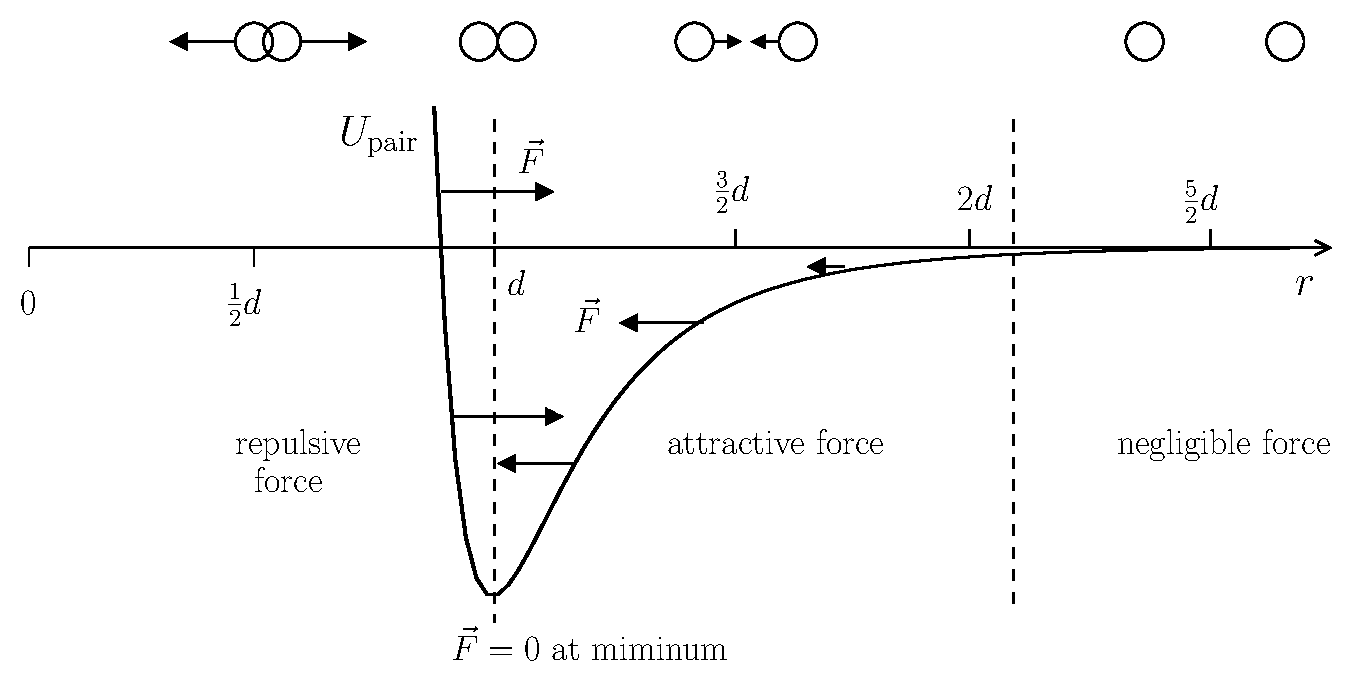
\includegraphics[width=5in]{thermal_energy_and_solids/pair_potential.eps}
\caption{The pair potential energy $U_\text{pair}$ as a function of
  $r$, the separation between the pair of molecules.  The dashed lines
  separate the regions of repulsive force, attractive force, and
  negligible force.  At separation $r=d$ the pair is in equilibrium,
  which defines the molecular diameter.}
\label{fig:pair_potential}
\end{center}
\end{figure}

What about other sources of potential energy besides the
intermolecular forces?  For example, gravitational potential energy.
When a ball is thrown upwards, the gravitational potential energy of
each molecule increases.  But the height of each molecule is increased
by the same amount that the height of the center of mass is increased.
Therefore this change in potential energy has the form
\begin{equation}
\Delta U_\text{grav} = M_\text{object} g\Delta y_{cm},
\end{equation}
where $M_\text{object}$ is again the total mass of the object.  This
is the familiar mechanical potential energy.  Therefore, gravitational
potential energy is always part of the mechanical energy, whereas the
molecular interaction energy makes up the thermal potential energy.

In summary, here is the big picture for thermal energy:
\begin{itemize}
\item For both potential energy and kinetic energy, it is the
  `organized' motion that makes up the {\it mechanical energy}, such as
  all molecules increasing their height together or all molecules
  having a net alignment of their velocities.
\item The remaining disorganized motion, such as the wiggling of the
  mole\-cules and their individual pushes and pulls on each other,
  corresponds to the {\it thermal energy}.
\item Friction is an agent that takes organized motion and
  disorganizes it, taking away mechanical energy and increasing thermal
  energy.
\item Going the other way --- taking away thermal energy and
  increasing mechanical energy --- is more difficult, since molecules
  are not likely to spontaneously start moving together.
  Nevertheless, we can capture some amount of thermal energy and
  convert it to mechanical energy with a device called a heat engine,
  which is the topic of Supplementary Reading Chapter
  \ref{chapter:heat_engines}.
\end{itemize}

\section{The Solid State}

\label{section:the_solid_state}

Molecules interacting via the pair potential can be solids, liquids,
or gases.  The remainder of this chapter is concerned with the thermal
energy of the solid state, while liquid and gas states will be
presented in Chapter \ref{chapter:liquids_and_gases}.


Most inorganic solids are crystalline, which means the molecules are
arranged in a symmetric way, such as a cubic lattice.  (Organic
  solids instead are constructed from long carbon chains.)  In this
lattice, each pair of neighboring molecules is separated by roughly
the equilibrium distance, that is, the minimum of the pair potential
well, and only makes small excursions from this location.  As
illustrated in Fig.~\ref{fig:pair_potential_spring}, the pair
potential in this region is identical to a parabolic potential.  We
have previously encountered a parabolic potential energy curve as the
potential energy for a mass on a spring.  Evidently, as long as the
molecules in a solid are not deviating significantly from their
equilibrium position, we may regard their interactions with their
nearest neighbors as equivalent to being attached by a spring.

\boxittext{{\sc Checkpoint:} What is the main difference between the pair
  potential and the spring potential?  What would I need to do to a
  pair of molecules to see this difference?  (Push together?  Pull
  apart?  How far?) }

\begin{figure}
\begin{center}
\includegraphics[width=3.5in]{thermal_energy_and_solids/pair_potential_spring.eps}
\caption{The solid curve is the pair potential $U_\text{pair}$ as a
  function of separation $r$.  The dashed line is the spring potential
  $U_\text{spring}$ with the spring constant $k_{\text sp}$ chosen to match
  $U_\text{pair}$ near the minimum.  The inset shows the match.}
\label{fig:pair_potential_spring}
\end{center}
\end{figure}


This leads to what we call the {\it ideal solid}:
the molecules are balls of mass $m$, they are connected by springs of
spring constant $k_\text{sp}$, and the springs have an equilibrium length
of $d$.  This model is illustrated in Fig.~\ref{fig:ball-spring}.  We
may think of the spring constant as determining the bond strength and
the equilibrium length $d$ as the bond length.  These three parameters
($m$, $d$, and $k_\text{sp}$) define the model, and we shall see that for
many solids determining these parameters describes much of the
behavior of the solid.

One may imagine packing the molecules together in different ways.  The
arrangement illustrated in Fig.~\ref{fig:ball-spring}, is called a
{\it simple cubic} lattice.  In fact, most solids are packed
differently, for example, in the way a grocer would stack oranges
(which is called a {\it face-centered cubic} lattice).  Fortunately,
this distinction has little impact on the quantities we will study, so
we will stick with the simple cubic lattice.

\begin{figure}
\begin{center}
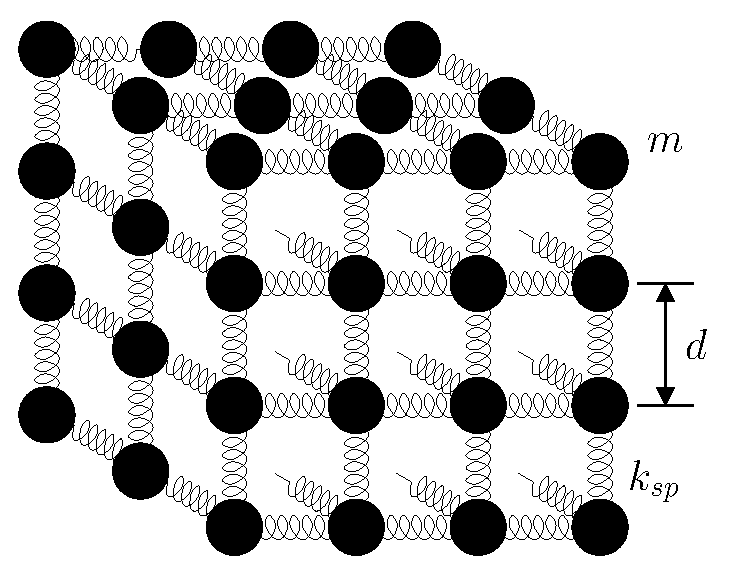
\includegraphics[width=2.5in]{thermal_energy_and_solids/ball-spring.eps}
\caption{The ball-spring model of a solid.}
\label{fig:ball-spring}
\end{center}
\end{figure}

Given the properties of some solid, how are the ideal solid
parameters determined?  Let's derive these for a specific case, namely
copper.  Molecular properties, such as mass, are usually not specified
for a single molecule, but rather for a {\it mole}.  One mole equals
Avogadro's number
\begin{equation}
N_A=6.02\times 10^{23}
\end{equation} 
of molecules.  Avogadro's number is chosen so that roughly one mole of
protons has a mass of one gram.  The precise definition is that one
mole of carbon atoms has a mass of $12\units{g}$.  The mass of one mole
of a material would logically be called the molar mass, but instead it
is usually called the {\it molecular weight}.\footnote{It's not our fault.}

One mole of copper has mass $64\units{g}$, so we may conclude that a
single molecule of copper (the ball in our model) has mass
\begin{equation}
m_\text{Cu} = \frac{64\units{g}}{6.02\times 10^{23}} = 1.06\times
10^{-22}\units{g}.
\end{equation}
This is the first of our three parameters.

Next, we can get the equilibrium spacing $d$ between the molecules by
knowing the density of copper, which is $8.94\units{g/cm$^3$}$.  
In Fig.~\ref{fig:ball-spring-volume} shows that each molecule of copper
occupies its own cubical region with volume $d^3$.
We can relate the density $\rho$ of the solid to the mass per volume
of a unit cell.  That is,
\begin{equation}
\rho = \frac{\text{mass}}{\text{volume}} = \frac{m}{d^3} 
  \qquad \Rightarrow\qquad d =
\left(\frac{m}{\rho}\right)^{1/3}.
\end{equation}
For copper this gives
\begin{equation}
d_\text{Cu} = \left(\frac{m_\text{Cu}}{\rho_\text{Cu}}\right)^{1/3}
 =  \left(\frac{1.06\times
     10^{-22}\units{g}}{8.94\units{g/cm$^3$}}\right)^{1/3}
 = 2.28\times 10^{-8}\units{cm},
\end{equation}
or equivalently, $2.28\times 10^{-10}\units{m}$.
And so we have the second parameter.

%Next, we can get the equilibrium spacing between the molecules by
%knowing the density of copper, which is $8.94\units{g/cm$^3$}$.  How
%many copper molecules are in a cubic centimeter of copper?    We can 
%calculate this as follows:
%\begin{equation}
%\frac{8.94\units{g}}{64\units{g/mole}} = 0.139 \units{mol}
% = 8.41\times 10^{22} \units{molecules},
%\end{equation}
%where Avogadro's number was used to convert moles to molecules.  The
%cubic centimeter of volume is divided equally among this number of
%molecules so the volume per molecule is
%\begin{equation}
%\frac{1 \units{cm$^3$}}{8.41\times 10^{22}\units{molecules}}
% = 1.19\times 10^{-23}\units{cm$^3$}.
%\end{equation}
%
%The volume for a single molecule can be pictured as a cube of length
%$d$, where $d$ is the bond length (see
%Fig.~\ref{fig:ball-spring-volume}).  Since the volume of a cube is
%$V=d^3$, the bond length is obtained from $d=V^{1/3}$, or
%\begin{equation}
%d = (1.19\times 10^{-23}\units{cm$^3$})^{1/3} = 2.28\times 10^{-8}\units{cm}
% = 2.28\times 10^{-10}\units{m}.
%\end{equation}
%And so we have the second parameter.

\begin{figure}
\begin{center}
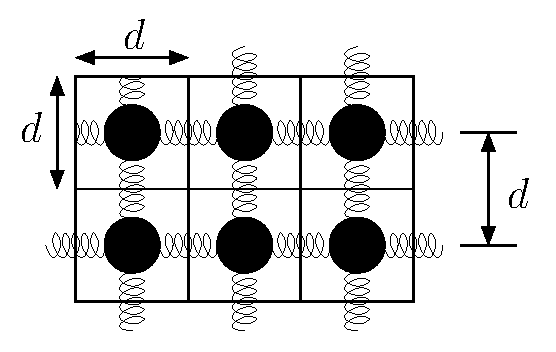
\includegraphics[width=2in]{thermal_energy_and_solids/ball-spring-volume.eps}
\caption{For the ideal solid with a separation $d$ between the 
balls, the volume per ball is given by a cube of side $d$ (shown here
in two-dimensions).}
\label{fig:ball-spring-volume}
\end{center}
\end{figure}


The final step is to determine the spring constant.  Fortunately, it
is not necessary to try pulling on a single molecule and measuring the
force that it pulls back with.  Rather, a macroscopic chunk of
material can be fixed at one end and pulled on the other, and by
measuring how much the object stretches, the bond spring constant can
be measured.

Imagine a piece of copper wire with cross-sectional area $A$ and
length $L$.  The applied force required to stretch the wire by an amount
$\Delta L$ is given by the following relation:
\begin{equation}
F_\text{app} = \frac{Y A}{L}\Delta L.
\label{eq:force_extension}
\end{equation}
This relation indicates that the amount of stretch $\Delta L$ is
proportional to the amount of force applied; doubling the force will
double the amount of stretch from the equilibrium length.  A larger
cross-sectional area $A$ makes the wire harder to stretch, which
accounts for the factor of $A$ in the numerator.  The longer the wire,
the easier it is to stretch, accounting for the factor of $L$ in the
denominator.  The final parameter $Y$ is called Young's modulus,
and is a property of the material but not dependent on the geometry
of the wire.  For example, Young's modulus for copper is
$Y_\text{Cu} \approx 130\times 10^9 \units{N/m$^2$}$.  

\begin{example}{Stretching an Extension Cord}
Consider 16 gauge copper wire, commonly used in power cables, which 
has a
cross-sectional area of $1.3\times 10^{-6}\units{m$^2$}$.  How much
force is required to stretch a 2-meter length of wire a distance of
1 centimeter?
\solution
According to Eq.~(\ref{eq:force_extension}), the force is given by
\begin{align}
 F_\text{app} = \frac{Y_\text{Cu}A}{L}\Delta L &=
 \displaystyle\frac{(130\times 10^9\units{N/m$^2$})(1.3\times
  10^{-6}\units{m$^2$})} {2\units{m}} (0.01\units{m}) \nonumber\\
 &= 845\units{N}.
\end{align}
\end{example} 

Now we need to calculate Young's modulus for the ideal solid.
Consider a rectangular solid of $N_x \times N_y \times N_z$ molecules.
The object is stretched in the $z$-direction by an applied force $F$,
with a resulting stretch $\Delta L$.  The stretch is shared equally
among each of the $N_z$ springs aligned in the $z$-direction, so each
spring is stretched an amount $\Delta L/N_z$.  The plane of molecules
where the force is applied consists of $N_xN_y$ molecules, each
connected to a spring pulling with force $k_\text{sp}\Delta L/N_z$.  This
spring force is balancing the applied force, so we can conclude that
\begin{equation}
F_\text{app}= N_xN_y \left(\frac{k_\text{sp} \Delta L}{N_z}\right).
\end{equation}
If we multiply top and bottom by $d^2$ we can identify the
cross-sectional area $A=(N_x d)(N_y d)$, and the length $L=N_z d$:
\begin{equation}
F_\text{app}=\frac{d^2N_xN_y k_\text{sp}}{d^2 N_z} \Delta L 
                = \frac{k_\text{sp}}{d}
\frac{A}{L}\Delta L
\end{equation}
from which we conclude that Young's modulus for the ideal solid
is
\begin{equation}
Y=\frac{k_\text{sp}}{d}.
\end{equation}
This can be used to find the spring constant, $k_\text{sp} = Yd$.  For
example, for copper
\begin{equation}
k_\text{sp} = (130\times 10^9\units{N/m$^2$})(2.28\times 10^{-10}\units{m})
 = 29.6\units{N/m}.
\end{equation}
In this way, we can find all three ideal solid parameters from
knowing the molecular weight, the density, and Young's modulus.


\section{Speed of Sound}
\label{section:speedofsound}

How well does this ball-spring picture of a solid work? 
One way to test the model is to study the speed of sound in a
solid.  Sound is a compression wave, much like a compression pulse
sent down a stretched slinky.  If an ideal solid is suddenly
struck at one end, how fast does the compression wave travel toward
the other end?  We can almost guess the answer.  The wave ``hops''
from one molecule to its neighbor and each hop moves the wave a
distance $d$.  Since the molecules are harmonic oscillators, the time
it takes for a hop must be related to the period of oscillation $T$,
so we could guess $v_\text{sound} \approx d/T$.  It is not difficult
to do the full calculation for the ideal solid\footnote{This is
  done in PHYS 221/222.} and find that the answer differs from this
guess by a factor of $2\pi$:
\begin{equation}
v_\text{sound} = \frac{2\pi d}{T} = d\omega  = d\sqrt{\frac{k_\text{sp}}{m}}
\end{equation}
Thus, the speed of sound in the ideal solid depends on all three
parameters.  The values we obtained for copper (be careful to use SI
units here!) give
\begin{equation}
 v_\text{sound} = 2.28\times
 10^{-10}\units{m}\sqrt{\frac{29.6\units{N/m}}{1.06\times
     10^{-25}\units{kg}}} = 3810\units{m/s}
\end{equation}
which is exactly the measured value for the speed of sound in copper.
Evidently the ideal solid model works quite well.  You will make more
comparisons in the homework.

\section{Temperature}

We began the chapter mentioning that when mechanical energy gets
converted to thermal energy, the temperature increases.  But what is
temperature?  Everyone has an intuitive feel for it:  we know that a
high temperature corresponds to something that is ``hot'' and a low
temperature corresponds to something that is ``cold.''  We also know
from experience that ``heat'' --- which we will define shortly --- flows
from hot (high temperature) to cold (low temperature) objects.

It is common in many introductory text books to define temperature as
a measure of the average thermal kinetic energy $K_\text{therm}/N$ of
a material.\footnote{Historically, this approach was used successfully
  in the $18^\text{th}$ and $19^\text{th}$ centuries to develop the
  first successful quantitative theories of thermodynamics, referred
  to as the {\em kinetic theory} of thermodynamics.}  This definition of
temperature is not valid for all situations (we will provide a more
rigorous definition of temperature in Chapter
\ref{chapter:second_law}); however, there are many situations that can
benefit from simple view of temperature as a measure of thermal
kinetic energy.

We must talk about temperature units.  The Celsius
temperature scale is defined so that water freezes at a temperature of
$0^\circ\units{C}$ and water boils at $100^\circ\units{C}$.  Considering
temperature as a measure of kinetic energy, we can define {\em absolute
zero} as the temperature where all molecular motion stops.  This occurs at
$-273.15^\circ\units{C}$ in the Celsius scale.  

\begin{figure}
\begin{center}
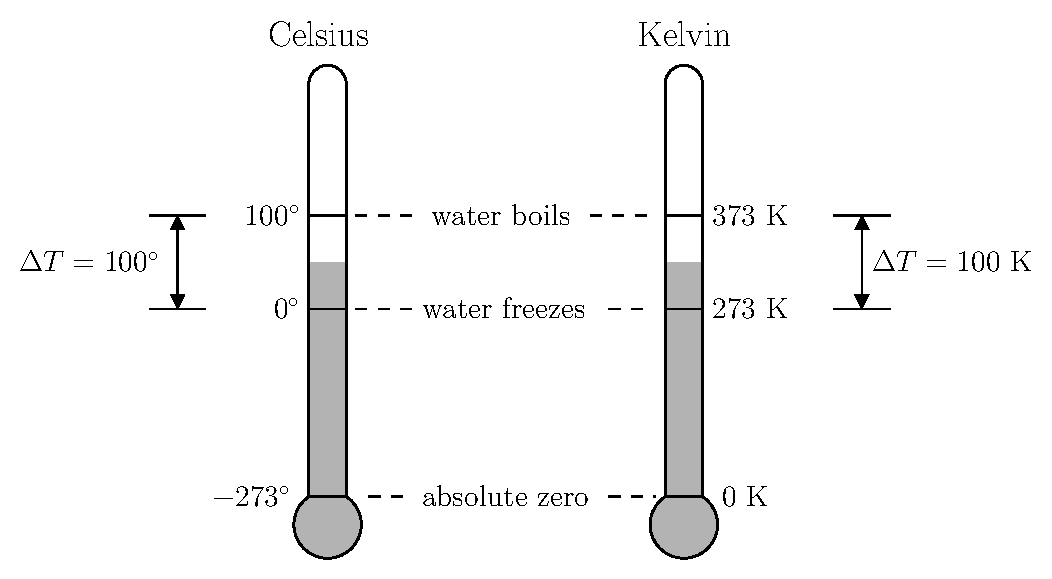
\includegraphics[width=4.5in]{thermal_energy_and_solids/temperature_scales}
\caption{The size of the degree is the same for Celsius and Kelvin
  temperature scales.  They differ by a shift:  $T_K=T_C+273$}
\label{fig:temperature_scales}
\end{center}
\end{figure}

A important variation on the Celsius temperature scale is called the
Kelvin scale, illustrated in Fig.~\ref{fig:temperature_scales}.  The
``size'' of the degree is the same for Kelvin and Celsius, that is, a
change in temperature of $1\units{K}$ is the same as a change in
temperature of $1^\circ\units{C}$.  The boiling temperature of water
is still $100\units{K}$ higher than the freezing temperature. The
difference in the scales is the location of zero: in the Kelvin scale,
absolute zero corresponds to $0\units{K}$, water freezes at
$273\units{K}$ and boils at $373\units{K}$.  The Kelvin temperature
scale is the one best suited for most thermodynamics problems.


\section{Molar Specific Heat}

Now we are prepared to address the question, ``If a certain amount of
thermal energy is added to a system, how much will the temperature
increase?''  This is a question with far-reaching applications.  For
instance, how much energy needs to be added to a swimming pool to heat
it up to a comfortable temperature?  How much cooling water or antifreeze
is needed to keep a car from overheating?  How much will the temperature
of a bucket of water increase if a hot ingot of lead is tossed into it?

We mentioned in the previous section that temperature is often associated
with the thermal energy of a system, i.e., increases in temperature
are associated with increases in the thermal energy.  But {\em how much}
does the temperature increase with a certain amount of energy is
added to a material?  For that, we define the {\em molar specific heat}
$C$:
\begin{equation}
C = \frac{\Delta E_\text{therm}}{n \Delta T}.
\label{eq:specificheat}
\end{equation}
In words, the specific heat is defined as the energy required to
raise the temperature of one mole of a material by a temperature 1 K.
So, a material with a large specific heat requires a lot of heat to
increase its temperature significantly, whereas a material with a
small specific heat requires less energy to raise its temperature by the
same amount.

Turning Eq.~(\ref{eq:specificheat}) around, the energy
required to raise the temperature of a material is given by
\begin{equation}
\Delta E_\text{therm} = n C \Delta T.
\label{eq:Ethermspecificheat}
\end{equation}
Measurements have been made of the molar specific heat for a wide
variety of materials.  A few of these values are listed in 
Table~\ref{table:material_properties} for some common metals.  

Note that the relation between the thermal
energy and the temperature depends on the amount of material via the
number of moles $n$. Having more stuff
will require more thermal energy to get the same temperature change.
The molar specific heat $C$, however, is defined such that it
does {\it not} depend on the amount of material.

\newpage

\begin{example}{Temperature increases}
How much thermal energy must be added to $5.0\units{kg}$ of lead to
increase its temperature from $25^{\circ}\units{C}$ to $40^{\circ}\units{C}$?

\solution First, it is convenient to determine how many moles of lead
we have here.  From Table~\ref{table:material_properties}, we see that
the molar mass of lead is $207\units{g/mol}$, so the number of moles
is given by
\begin{equation*}
n = 5.0\units{kg} \cdot \frac{1000\units{g}}{\units{kg}} \cdot 
\frac{1\units{mol}}{207\units{g}} = 24.2\units{mol}
\end{equation*}
From Table~\ref{table:material_properties}, we see that
the molar specific heat of lead is 
$26.6\units{$\frac{\rm J}{\rm mol} \cdot {\rm K}$}$.
Using Eq.~(\ref{eq:Ethermspecificheat}), we find
\begin{equation*}
\Delta E_\text{therm} = n C \Delta T = 24.2\units{mol} \cdot
26.6\units{$\frac{\units{J}}{\units{mol} \cdot \units{K}}$} \cdot 15\units{K} = 9640\units{J}.
\end{equation*}
Note that the conversion between Celsius and Kelvin is trivial; a
temperature difference of $15^{\circ}\units{C}$ is the same as a
temperature difference of $15\units{K}$.
\end{example}

Looking at Table~\ref{table:material_properties}, it is apparent that
the molar specific heat for metals is fairly consistent --- around 
$25\units{J/mol$\cdot$K}$ --- for several common metals.  A pattern like this
indicates that there might be a simple, common explanation.  That
explanation is provided by the ideal solid model and what is known as the
equipartition theorem.

\section{The Equipartition Theorem}
\label{sec:equipartition}

We now discuss a remarkable relationship between temperature and
thermal energy, referred to as the {\em equipartition theorem}.  The
basic idea is that in thermodynamic systems, thermal energy is equally
(``equi'') divided (``partition'') between certain types of molecular
energy, both kinetic and potential.  At first glance, you might think
that this would mean that half of the energy is kinetic and half is
potential (and sometimes this is true), but it is not quite that simple.
For one, only those energy terms which are quadratic in a
dynamical variable (such as $\frac{1}{2}mv_x^2$) get the equal shares.
For any terms more complicated than that, like the pair potential, we
cannot so easily say how the energy is divided.  Also, the number of these
egalitarian quadratic energy terms, often called {\it degrees of freedom},
depends on details such as whether there is rotational as well as
translational kinetic energy.\footnote{For a solid the molecules
  essentially do not rotate, but rotational kinetic energy can have a
  significant effect on the thermal energy of a liquid or gas.}


% because (a) there are different types of kinetic
%energy, e.g., translation and rotational\footnote{For a solid the
%molecules essentially do not rotate, but rotational kinetic energy
%  can have a significant effect on the thermal energy of a liquid
%  or gas.} kinetic energy; (b) the partition of energy also depends on
%the number of {\em degrees of freedom} a system has, e.g., whether a
%molecule can oscillate only in one direction (1 degree of freedom),
%along a plane (2 degrees of freedom) or in any of the three dimensions
%(3 degrees of freedom); and (c) it only applies to {\em quadratic}
%degrees of freedom, meaning the energy term has to be proportional to
%the variable squared.

Maybe it will help to see the theorem:

\boxittext{{\sc Equipartition Theorem:}\\[0.5ex]
  Any term in the energy of a
  molecule that is quadratic, such as $\frac{1}{2}mv_x^2$ or
  $\frac{1}{2}k_\text{sp}x^2$ or $\frac{1}{2}I\omega^2$, averages to
  $\frac{1}{2}k_BT$.}

This amazing result says that when some $10^{23}$ particles push and pull
and collide with each other, all the messy forces involved will result in
every quadratic energy term averaging to the same value.   It doesn't
matter if the molecule is heavier or lighter, or what the spring
constant is.  It also doesn't matter whether we are talking about
potential energy or translational kinetic energy or rotational kinetic
energy.  As long as the energy is quadratic in the dynamical variable, 
the thermal energy will depend only on $T$ and
Boltzmann's constant,
\begin{equation}
k_B= 1.38\times 10^{-23}\units{J/K},
\end{equation}
which is another constant of nature.  Notice how the units work out:
$k_BT$ is an energy.

%As an example, let's say that we have a gas composed of N non-interacting
%atoms (i.e., neglecting any forces between them), each of which 
%can move in the $x-$, $y-$ or $z-$directions.
%The energy of one of these atoms is then
%\begin{equation*}
%E_\text{atom} = 
%{\textstyle\frac{1}{2}}mv_x^2 +
%{\textstyle\frac{1}{2}}mv_y^2 +
%{\textstyle\frac{1}{2}}mv_z^2.
%\end{equation*}
%(There are no potential energy terms here because we are neglecting
%interactions between the atoms.)
%According to the equipartition theorem, each of these three terms
%averages to ${\textstyle\frac{1}{2}}k_BT$, so the average energy
%per atom is
%\begin{equation*}
%\langle E_\text{atom}\rangle = 3\left({\textstyle\frac{1}{2}}k_BT\right) 
%= {\textstyle\frac{3}{2}}k_BT.
%\end{equation*}
%and the total thermal energy for the system is simply
%\begin{equation*}
%E_\text{therm,gas} = N ({\textstyle\frac{3}{2}}k_B T)
%\label{eq:E_thermalgas}
%\end{equation*}
%Note how quick this result is.  We don't have to worry about any of
%the details of the individual atoms in the gas.  The equipartition
%theorem takes care of all of that for us.

In the next sections, we'll use the equipartition theorem to analyze
thermal energy of an ideal solid.

\section{Ideal Solid Specific Heat}

To determine the molar specific heat of an ideal solid,
let us make the approximation that the neighbors of
a particular molecule remain fixed.  This turns out to be a reasonable
approximation for most solids.  Then the energy describing that
particular molecule is
\begin{equation}
E_\text{molecule} = {\textstyle\frac{1}{2}}mv_x^2 +
{\textstyle\frac{1}{2}}mv_y^2 + {\textstyle\frac{1}{2}}mv_z^2 +
{\textstyle\frac{1}{2}}k_\text{sp}x^2 + {\textstyle\frac{1}{2}}k_{\rm sp}y^2 +
{\textstyle\frac{1}{2}}k_\text{sp}z^2.
\label{eq:ball-spring_energy}
\end{equation}
There are six terms contributing to the energy, all of which are
quadratic.  Each term is fluctuating up and down as the molecule
interacts with its neighbors.  The equipartition theorem tell us,
then, that the average energy of this ball over time will be
\begin{equation}
\langle E_\text{molecule}\rangle =
6\left({\textstyle\frac{1}{2}}k_BT\right) = 3k_BT.
\end{equation}
Now consider an $N$ molecule ideal solid.  The number of moles
is given by $n = N/N_A$, and the 
thermal energy will be
\begin{equation}
E_\text{therm} = N (3 k_B T) = \frac{N}{N_A}(3k_BN_A)T = n3RT,
\quad\text{(ideal solid)}
\label{eq:E_thermal}
\end{equation}
where $R=N_A k_B = 8.31\units{J/mol$\cdot$K}$ is called the gas
constant, although it has nothing in particular to do with
gases.\footnote{This isn't our fault either.}  

Comparing Eqs.~(\ref{eq:E_thermal}) and (\ref{eq:Ethermspecificheat}),
the molar specific heat of the ideal solid is
\begin{equation}
C = 3R = 24.9\units{J/mol$\cdot$K} \qquad\text{(ideal solid)}
\end{equation}
regardless of the material.  This relation is known as the
Dulong-Petit law.  The molar specific heats of most solids agree with
the Dulong-Petit result to within a few percent accuracy.  For
example, the molar specific heat of copper is $C_\text{Cu} =
24.4\units{J/mol$\cdot$K}$, and comparable values for a variety of
other solids are given in Table~\ref{table:material_properties}.  This
provides more evidence that the ball-spring model of the ideal solid
is reasonable.


\begin{table}
\begin{tabular}{lccccc}
\hline\hline
Material & $M$ (g/mol) & $\rho$ (g/cm$^3$) & $Y$ (GN/m$^2$) & 
$C$ (J/mol$\cdot$K)  & $v_s$ (m/s) \\ \hline
% & (g/mol) & (g/cm$^3$) & (GN/m$^2$) & (J/mol$\cdot$K) & (m/s)\\ \hline
Aluminum & 27.0 & 2.70 & 70  & 24.2  & 5000\\
Iron     & 55.8 & 7.87 & 211 & 25.1  & 5120\\
Copper   & 63.5 & 8.96 & 130 & 24.4  & 3810\\
Gold     & 197  & 19.3 & 78  & 25.4  & 2030\\
Lead     & 207  & 11.3 & 16  & 26.6  & 1190\\
ideal solid & $mN_A$ & $m/d^3$ & $k_{\rm sp}/d$ & 3R = 24.9  
                                          &  $d\sqrt{k_{\rm sp}/m}$\\
\hline\hline
\end{tabular}
%\caption{Material properties for a few selected substances.}

% \begin{tabular}{lccccc}
% \hline\hline
% Material & $M$ (g/mol) & $\rho$ (g/cm$^3$) & $Y$ (GN/m$^2$) & 
% $C$ (J/mol$\cdot$K)  & $v_s$ (m/s) \\ \hline
% % & (g/mol) & (g/cm$^3$) & (GN/m$^2$) & (J/mol$\cdot$K) & (m/s)\\ \hline
% Aluminum & 27.0 & 2.70 & 70  & 24.2  & 5000\\
% Iron     & 55.8 & 7.87 & 211 & 25.1  & 5120\\
% Copper   & 63.5 & 8.96 & 130 & 24.4  & 3810\\
% Gold     & 197  & 19.3 & 78  & 25.4  & 2030\\
% Lead     & 207  & 11.3 & 16  & 26.6  & 1190\\
% ideal solid & $mN_A$ & $m/d^3$ & $k_\text{sp}/d$ & 3R = 24.9  
%                                           &  $d\sqrt{k_\text{sp}/m}$\\
% \hline\hline
% \end{tabular}
\caption{Material properties for a few selected substances.}
\label{table:material_properties}
\end{table}

Finally, note that the specific heat is only defined in terms of
$\Delta E_\text{therm}$ and $\Delta T$; it relates {\it changes} in
the temperature to changes in thermal energy.  However, if we assume
that the specific heat is independent of temperature, which is a
reasonable approximation down to some low temperature, then we can
also estimate
\begin{equation}
E_\text{therm} \approx nCT = n3RT. \qquad\text{(ideal solid)}
\end{equation}


\section{Heat and the First Law of Thermodynamics}
\label{section:heat}

There are many ways to add thermal energy to an object or to remove it
from the object.  We have already discussed how friction can increase
the thermal energy of a blow dart as it slides across the floor.
Another way to change the thermal energy is to bring the object into
{\it thermal contact} with something hotter or colder.  For a pair of
solid objects, thermal contact occurs when they are physically in
contact.  Then the molecules at the boundary exert forces on each
other and energy is transferred from the object with the higher
temperature to the object with the lower temperature.  
As we have already discussed,  temperature directs the flow of
thermal energy, determining which objects will spontaneously give off
energy and which objects will receive it.

The energy transferred spontaneously by molecular motion is given the
name {\it heat.}  Similar to work, heat is an energy transfer and not
an energy.  Think of thermal energy as a bank balance and heat and work
as deposits and withdrawals.  The distinction between heat and
work is the mechanism for the energy transfer.

\boxittext{Heat is the thermal energy transferred spontaneously due
to a temperature difference.}

\noindent All other forms of energy transfer into a system are lumped 
together as thermodynamic ``work."  For example, the term work can refer 
to energy transfer due to external forces that act on system (but do not 
change the motion of the center of mass of the system)\footnote{In Unit 1 
in this course we discussed the work done on a single particle,
and the resulting change in the kinetic energy of the particle.
In thermodynamics we are interested in composite systems, such as gases
liquids, and solids.  In composite systems, work can result in changes in
thermal energy as well as kinetic energy. In the thermodynamic systems
we study, there will be no changes in the bulk kinetic energy 
$K_\text{mech}$.}, but it also 
encompasses energy transfers due to other things, such as the warming of 
a piece of frozen broccoli in a microwave oven.  To distinguish the 
two forms of energy transfer, it is common to use the symbol $Q$ for heat, 
and $W$ for work.

Now we can state the first law of thermodynamics, which is simply a
statement of energy conservation: the change in thermal energy is
equal to how much work is done on the system plus how much heat flows
into the system:
\begin{equation}
\Delta E_\text{therm} = Q + W \qquad\text{(1st Law of Thermodynamics)}
\end{equation}
Note that $Q$, like $W$, can be positive or negative, depending on
whether heat is flowing in or out.  The convention used here is to
define the heat $Q$ as being positive if heat is flowing {\em into}
the material (and negative if heat is flowing out), and to define
the work $W$ as the work done {\em on} the system.  Some people find it
convenient to write the first law with these conventions stated
explicitly:
\begin{equation}
\Delta E_\text{therm} = Q_\text{in} + W_\text{on} \qquad\text{(1st Law of Thermodynamics)}
\label{eq:firstlaw}
\end{equation}

From our perspective today, with energy conservation a fundamental
principle, the 1st law may seem to be pretty obvious.  But historically it was a
very significant discovery, showing that indeed heat was just an
energy transfer, rather than some new substance.\footnote{Early theories of
thermodynamics proposed -- incorrectly -- that heat was some sort of
fluid (called {\em caloric}) that flows between hot and cold materials.
We now know, of course, that heat is simply the ``flow'' of energy.}
And the
importance of the first law cannot be overstated -- this seemingly simple
result forms the foundation of much of what we will be doing during
the next couple of weeks.

It is worth appreciating what is not heat.  Rubbing your hands
together when they are cold certainly does increase their thermal
energy, but not due to heat.  There is not a higher temperature object
making energy flow into your hands spontaneously, so there is no heat
flow.  Rather, you are doing work with your muscles, and the friction
force between your hands converts the mechanical energy of your moving
hands into thermal energy.

\begin{example}{First law}
You hold a $35\units{mol}$ iron anvil in place on a moving conveyor belt
so that the belt slides under the stationary anvil. The belt does 
$12,000\units{J}$ of work on the anvil, and and it gets warmer. During 
this process, the anvil loses $7,000\units{J}$ to the cooler surrounding air 
and to the belt.  If the anvil had an initial temperature of 
$22.0^{\circ}\units{C}$, what is its temperature at the end of this 
process?

\solution
First, we can use the first law to determine the change in the anvil's
thermal energy.  Conceptually, $12,000\units{J}$ is  added in the form
of work and $7,000\units{J}$ is removed in the form of a heat flow.  In terms
of Eq.~(\ref{eq:firstlaw}), $W_\text{on}=12000\units{J}$ and 
$Q_\text{in}=-7000\units{J}$ (negative since heat is flowing {\em out}
of the anvil).  So,
\begin{equation*}
\Delta E_\text{therm} = Q_\text{in} + W_\text{on} 
     = -7000\units{J} + 12000\units{J}= 5000\units{J}.
\end{equation*}
We can now use Eq.~(\ref{eq:Ethermspecificheat}) and the molar specific
heat of iron (see Table~\ref{table:material_properties} to find the
temperature change of the iron anvil:  
\begin{equation*}
\Delta E_\text{therm} = n C \Delta T.
\end{equation*}
Solving for the rise in temperature gives
\begin{eqnarray*}
\Delta T &=& \frac{\Delta E_\text{therm}}{nC} \\
         &=& \frac{5000\units{J}}{35\units{mol} \times 25.1\frac{\units{J}}
{\units{mol} \cdot \units{K}}} \\
         &=& 5.7\units{K}
\end{eqnarray*}  
The final temperature is therefore $22.0^\circ\units{C} + 5.7^\circ\units{C} = 
27.7^\circ\units{C}$.


Note that we could get a very good approximation of the result here by using
the ideal solid approximation for the molar
specific heat.

\end{example}


When a pair of objects is in thermal contact but is otherwise thermally
isolated, we can say that $\Delta E_\text{therm}$ is equal and opposite
for the two objects, since the thermal energy lost by the hotter object
is gained by the colder object.  This brings the objects closer together
in temperature, until finally they have the same temperature and no more
heat flows.  This situation is called {\it thermal equilibrium}.

\begin{example}{Hot Meets Cold}
One mole of an ideal solid at temperature $70^\circ\units{C}$ is
brought into thermal contact with two moles of an ideal solid at
temperature $10^\circ\units{C}$.  How much heat will flow out of the
hotter object before thermal equilibrium is reached?
 
\solution 
We will need to
determine the final equilibrium temperature, $T_f$.  
This is done by balancing the heat flows in and out:
\begin{equation} 
\Delta
E_\text{therm,1} = -\Delta E_\text{therm,2} 
\>\Rightarrow\>
n_1 C_1 \underbrace{(T_f - T_{1,i})}_{\Delta T_1} = -n_2 C_2 
\underbrace{(T_f - T_{2,i}) }_{\Delta T_2}
\label{eq:calorimetry}
\end{equation}
where $T_{1,i}$ and $T_{2,i}$ are the initial temperatures of objects
1 and 2.  Putting in values:
\begin{equation}
(1\units{mol})(3R)(T_f - 70^\circ\units{C})
 = -(2\units{mol})(3R)(T_f - 10^\circ\units{C})
\end{equation}
Note that we have used Celsius temperature.  This is because $\Delta
T$ is the same whether measured in Kelvin or Celsius (see
Fig.~\ref{fig:temperature_scales}).  Now we solve:
\begin{equation}
T_f - 70 = -2(T_f-10)\quad\Rightarrow\quad 3T_f = 70+20
\end{equation}
so
\begin{equation}
T_f = \frac{90}{3} = 30^\circ\units{C}.
\end{equation}
To complete the calculation, we go back to the change in thermal energy,
Eq.~(\ref{eq:calorimetry}),
\begin{equation}
\Delta E_\text{therm,1} = (1\units{mol})(24.9\units{J/mol$\cdot$K})
(30^\circ\units{C} - 70^\circ\units{C}) = -996\units{J}.
\end{equation}
So $996\units{J}$ of heat flowed out of object $1$ and into object $2$.
\end{example}



\newpage

\section*{Problems}
\markright{PROBLEMS}

\begin{problem}
  To understand better how the ideal solid thermal energy
  is derived, consider the following scenario.
  A mad scientist creates a new material, flattium, in which the
  molecules can only move in the $x$-$y$ plane, while their $z$
  coordinates remain fixed.  Consider how
  Eq.~(\ref{eq:ball-spring_energy}) would be changed, and then use
  the equipartition theorem to derive an expression for the thermal energy of
  flattium.
\label{problem:flattium}
\end{problem}

\begin{problem}
  Here is some practice with the ideal solid model.
\begin{enumerate}
\item Using the data in Table~\ref{table:material_properties},
  determine the ideal solid parameters, $m$, $d$, and $k_\text{sp}$,
  for iron.
\item Use these values to estimate the speed of sound in iron.
  Compare your answer with the measured value.
\end{enumerate}
\label{problem:ball-spring_iron}
\end{problem}

\begin{problem}
  Determine the thermal energy of one mole of a solid at a temperature of
  $100^\circ\units{C}$.  You can use the ideal solid
  approximation for the molar specific heat.
  \label{problem:iron_E_thermal}
\end{problem}


%\begin{problem}
%  Consider one-molar chunks of iron and copper at the same temperature
%  $T$.  Use your results from problem \ref{problem:ball-spring_iron}
%  and the ball-spring parameters for copper given in section
%  \ref{section:the_solid_state} to answer the following questions:
%  \begin{enumerate}
%  \item Which of the two materials has a greater thermal kinetic
%    energy, or are they equal?
%  \item Which of the two materials has on average faster moving
%   molecules, that is, a higher average for $v^2$, or are they equal?
%  \end{enumerate}
%  \label{problem:compare_iron_copper}
%\end{problem}


\begin{problem} 
  Calculate the thermal energy required to raise the temperature of
  iron by $25\units{K}$ for the amounts given below.
\begin{enumerate}
\item One mole of iron.
\item One gram of iron.
\item One cubic centimeter of iron.
\end{enumerate}
\label{problem:mole_kg_cc}
\end{problem}


\begin{problem}
  A two-mole ideal solid at temperature $40^\circ\units{C}$ is
  brought into thermal contact with a one-mole ideal solid at
  temperature $10^\circ\units{C}$.  Energy flows from the hotter solid
  to the colder solid until they reach the same final temperature.
\begin{enumerate}
\item Calculate the final temperature.
\item Calculate the amount of thermal energy transferred in this process.
\end{enumerate}
\label{problem:calorimetry}
\end{problem}

\begin{problem}
  Using your results from Problem \ref{problem:ball-spring_iron},
  calculate the typical period of oscillation for an iron molecule
  at $50^\circ\units{C}$.
\label{problem:iron_oscillation}
\end{problem}

\begin{problem}
  A 20 kg brick of lead is dropped from a height of $5.0\units{m}$
  above the sidewalk.  It falls to the ground where it comes to rest.
  Assume that 60\% of the mechanical energy of the brick is converted
  to thermal energy of the brick (the remaining energy went into
  thermal energy of the sidewalk and a big crack).  Determine the
  temperature increase of the brick. {\it Hint:} you will need to
  calculate how many moles of lead the brick contains. 
\label{problem:falling_brick}
\end{problem}


\begin{problem}
  For silver, the ideal solid parameters are $m=1.79\times
  10^{-25}\units{kg}$, $d=2.58\times 10^{-10}\units{m}$, and
  $k_\text{sp}=21.4\units{N/m}$.  Based on this information, calculate the
  density and Young's modulus for silver.
\label{problem:silver_ball-spring}
\end{problem}

\begin{problem}
  In the following list of processes, the thermal energy of an object
  is increasing (and so the temperature is increasing as well).  For
  which processes is this increase due to heat flow?
\begin{enumerate}
\item a drill bit which has been used to bore a hole
\item an ice cube placed in a glass of water
\item a cup of coffee warming in a microwave
\item the filament in a light bulb in a lamp that is plugged in and turned on
\item cookies placed into an oven to bake
\end{enumerate}
\label{problem:heat_examples}
\end{problem}

\begin{problem}
  Consider three bricks, all with mass $10\units{kg}$ and at room
  temperature. The first brick is made of aluminum, the second brick
  copper, and the third brick lead.  Which will have the largest thermal
  energy?  Rank from from highest to lowest.
\label{problem:compare_heat_capacity}
\end{problem}

\begin{problem}
\begin{enumerate}
\item Using the data in Table~\ref{table:material_properties}, 
determine the ideal solid
parameters, $m$, $d$, and $k_\text{sp}$, for aluminum.
\item Use these values to estimate the speed of sound in aluminum.  Compare
your answer with the measured value.
\end{enumerate}
\end{problem}

%\begin{problem}
%  Consider one-molar chunks of iron and copper at the same temperature
%  $T$.  Use your results from problem \ref{problem:ball-spring_iron}
%  and the ball-spring parameters for copper given in section
%  \begin{enumerate}
%  \item Which of the two materials has a greater thermal potential
%    energy, or are they equal?
%  \item Which of the two materials has on average molecules wandering
%    farther from their equilibrium position, that is, a higher average
%    for $x^2$, or are they equal?
% \end{enumerate}
%\end{problem}

\begin{problem}
  For an ideal solid at temperature $T$, determine the ratio of
  thermal kinetic energy to thermal potential energy.  Use the
  equipartition theorem to justify your answer.
\end{problem}


\begin{problem}
Specific heats are often given by the amount of thermal energy
required to raise the temperature of {\it one kilogram} of material by
a degree, rather than {\it one mole} of material.  The per-kilogram
specific heat $c$ satisfies $\Delta E_\text{therm} = m_\text{obj} c
\Delta T$, where $m_\text{obj}$ is the mass of some object. Calculate
the per-kilogram specific heat of iron.
\end{problem}


\begin{problem}
  Ideal solid {\bf A} containing one-mole at some initial temperature $T_A$ is
  brought into contact with ideal solid {\bf B} containing three moles at
  temperature $20^\circ\units{C}$.  The system equilibrates at a
  temperature of $75^\circ\units{C}$.
\begin{enumerate}
\item Calculate the initial temperature of the solid {\bf A}.
\item Calculate the amount of thermal energy transferred.
\end{enumerate}
\end{problem}


\begin{problem}
Thermal energies are large!  Calculate (roughly) the thermal energy of an
$8\units{kg}$ brick of lead at room temperature, say
$22^\circ\units{C}$.  Compare this to the gravitational potential
energy of lifting this brick a height of $2\units{m}$.
\label{problem:thermal_energies_large}
\end{problem}

\begin{problem}
In Section \ref{section:the_solid_state}, an equation was derived to
determine the spring constant $k_\text{sp}$ for the ball-spring model from
the value of the Young's modulus for a material:  $k_\text{sp} = Yd$.
\begin{enumerate}
\item Show that this equation gives the proper units for the spring
constant, given the units for $Y$ and $d$.
\item Write a sentence explaining why it makes sense that a material
with a large Young's modulus is associated with a large spring constant
$k_\text{sp}$ for interactions between adjacent atoms.
\end{enumerate}
\end{problem}

\begin{problem}
In Section \ref{section:speedofsound}, an equation was derived to
determine the sound speed:
\begin{equation*}
v_\text{sound} =  d\sqrt{\frac{k_\text{sp}}{m}}.
\end{equation*}
\begin{enumerate}
\item Show that this equation gives the proper units for the speed
of sound, given the units for $d$, $k_\text{sp}$ and $m$.
\item Write a sentence explaining why it makes sense that a material
with a large $k_\text{sp}$ is associated with a large speed of sound.
\item Write a sentence explaining why it makes sense that
the speed of sound is smaller for a material whose atoms have a 
larger molar mass. 
\end{enumerate}
\end{problem}

\begin{problem}
You do $275\units{J}$ of work on a system, and its thermal energy 
increases by $530\units{J}$.  Calculate the heat that flows into 
or out of the system, and specify which direction the heat flows 
(i.e., in or out).
\end{problem}

\begin{problem}
You are polishing a $5.0\units{g}$ gold wedding ring.  After doing
this for a minute, you find that the ring is hot, having warmed up
$20^{\circ}\units{C}$.  Assuming that the ring loses $210\units{J}$
to the air while you are polishing it, calculate the work that you did
on the ring while polishing it.
\label{prob:polish_ring}
\end{problem}


\input{liquids_and_gases/liquids_and_gases}

\input{gas_processes/gas_processes}

%\input{gas_processes/test.tex}

\input{second_law_and_entropy/second_law_and_entropy}

\chapter{Heat Engines}
\label{chapter:heat_engines}

\section{Introduction}

Mechanical energy is essential for our every day life: cars move
along roads and highways, electrons flow through 
semiconductor devices in our iPods,
and blood flows through our arteries.  Mechanical energy makes matter
do things, and converting other forms of energy to mechanical energy
is an essential technological challenge.  Batteries and our bodies
convert chemical bond energy into mechanical energy.  And nuclear reactors
convert mass into mechanical energy.

But we have seen that there is a considerable amount of energy
contained in the disorganized thermal motion of the molecules and the
disorganized pushes and pulls on their molecular neighbors.
Harnessing some of this thermal energy and converting it to organized
mechanical energy provides yet another source of mechanical energy.
But just how do we go about doing this?

It is tempting to imagine some kind of molecular referee who could
convince the all the molecules in a material to align their motion.
If the molecules in your textbook could do this, your book would zip
away from you at many hundreds of miles per hour, so it would be a
very useful trick.  However, no such microscopic referee exists.  In
fact, this trick would violate the second law of thermodynamics,
moving from a more probable to a less probable arrangement of
velocities.\footnote{This microscopic referee was first pondered by
  Maxwell, and is commonly referred to as Maxwell's Demon.  He showed
  that the referee could make heat flow from a colder object to a
  hotter one --- in contradiction to the second law, which of course
  is impossible.}

Nevertheless, it is still possible to convert some (but not all)
thermal energy to mechanical energy.  That is, we can design devices
to do this while still satisfying the second law.  These devices are
called {\it heat engines}, and they played an essential role in the
industrial revolution and continue to play a vital role in modern
society.

In this chapter we will study the basic physics behind heat engines.
We will discuss how the basic principle of a heat engine can be
understood using the arguments of statistics and entropy discussed in
Chapter \ref{chapter:second_law}.  We will also describe the basic gas
cycles that many such engines employ.  As a fundamental starting
point, any heat engine must satisfy the second law of thermodynamics,
$\Delta S_\text{total} \ge 0$, so we begin with developing a
convenient and powerful relationship between entropy change and heat.

\section{Entropy Change and Heat}

As discussed in the previous chapter, entropy is a measure of
probability; specifically, it is Boltzmann's constant times the
logarithm of the multiplicity.  While we can work with the
multiplicity and take logarithms for simple enough models, we often
want to know the entropy (actually, the entropy {\it change} $\Delta
S$) for more complicated situations without having to sort out exactly
what is going on with the multiplicity.

In many situations it is possible to do this.  We begin with our
result from the previous chapter:
\begin{equation}
\frac{1}{T} = \frac{dS}{dE_\text{therm}},
\end{equation}
which we can rewrite as a relation between a small (infinitesimal) entropy
change $dS$ and a small thermal energy change $dE_\text{therm}$,
\begin{equation}
dS = \frac{dE_\text{therm}}{T} \qquad(W=0).
\label{eq:dSdEtherm}
\end{equation}
In our development of the definition of temperature, we only
considered energy transfers between subsystems $A$ and $B$ that
happened spontaneously, due to the increased probability associated
with the new energy distribution.  In other words, we only allowed for
thermal energy changes due to {\it heat} and not due to {\it work}.
Hence the $W=0$ label in Eq.~(\ref{eq:dSdEtherm}).

Recall that the first law of thermodynamics, for small amounts of heat
and work, says
\begin{equation}
dE_\text{therm} = dQ + dW.
\end{equation}
If no work is being done, $dE_\text{therm}$ is the same thing as $dQ$:
the thermal energy has changed by however much heat flow has occurred.
Thus, we could equally well write Eq.~(\ref{eq:dSdEtherm}) with a $dQ$
in the numerator.

So the question is, what is the appropriate generalization of
Eq.~(\ref{eq:dSdEtherm}) to cases where there is both heat flow and
work done?  Should the numerator still be $dE_\text{therm}$, or should
it be $dQ$, or something else entirely?

The answer is: it depends.  If the work is being done slowly enough
that the system remains in thermal equilibrium (which means that the
basic hypothesis of all microstates being equally likely is at all
times still true), then we have a clear answer: the numerator should
be $dQ$, and so
\begin{equation}
dS = \frac{dQ}{T}  \qquad\text{(whether or not $W=0$)}.
\label{eq:dSdQ}
\end{equation}
A good rule of thumb for ``slow enough'' is that whatever moving
object is doing the work should move slower than the speed of sound.
In many cases this isn't much of a limitation.  For our purposes, we
will assume that we remain in equilibrium for all the processes we
consider.\footnote{When this isn't the case, and the system goes out
  of equilibrium, we do not have a general expression for the change
  in entropy.  This is an active area of research today!}

But you may be wondering why doing work (slowly enough) doesn't affect
the entropy, that is, $\Delta S$ only depends on the heat flow.  The
full explanation is beyond the scope of this course, but here is the
flavor of it.  We could do work on a solid by squeezing it, and this
would certainly increase the thermal energy.  The Einstein solid of
the previous chapter would respond to the squeezing by having an
increased energy spacing $\epsilon$, but not by having more ``energy
units.''  So the multiplicity wouldn't change, even though the thermal
energy has gone up.  And of course if the multiplicity doesn't change,
the entropy doesn't change.

In practical terms, Eq.~(\ref{eq:dSdQ}) is a very handy tool for
calculating entropy changes.  Of course, we usually have more than a
small amount of heat flow, so we will need to use calculus to add up
the net entropy change:
\begin{equation}
\Delta S = S_B - S_A = \int_A^B dS = \int_A^B \frac{dQ}{T}.
\qquad\text{(equilibrium processes)}
\label{eq:DeltaSgeneral}
\end{equation}

Often we are considering constant temperature situations, and then
this result simplifies even further:
\begin{equation}
\Delta S= \frac{1}{T}\int dQ = \frac{Q}{T} \qquad\text{(constant temperature)}
\label{eq:deltaS_isothermal}
\end{equation}
The sign of $Q$ is important here!  When $Q$ is positive, $\Delta S$
is positive, and when $Q$ is negative, $\Delta S$ is negative.  Or to
put it another way: heat flow in increases the entropy, and heat flow
out decreases the entropy.  {\bf Do not forget this!}  The second law
is commonly misunderstood to say that all entropies must always
increase.  This is simply not true.  The second law only tell us the
{\it total} entropy must increase.

There are three common situations where the temperature is constant,
even though heat is flowing in or out of the system.
\begin{itemize}
\item {\it for an isothermal process} --- isothermal expansion or
  contraction of a gas is, by definition, at constant temperature (iso
  = ``equal'', thermal = ``temperature'').
\item {\it during a phase change} --- the latent heat at a phase
  transition (e.g., melting/solidifying or vaporizing/condensing)
  keeps the temperature constant.
\item {\it for a thermal reservoir} --- if a system is very large,
  modest amounts of heat flow will not affect the temperature.  For
  example, dumping a cup of coffee into the ocean will not change the
  ocean's temperature measurably.
\end{itemize}

\begin{example}{Entropy Change of Melting Ice}
  Consider an $18\units{g}$ ice cube at $0^\circ\units{C}$.  Heat
  flows in until is has changed phase to $0^\circ\units{C}$ water.
  The water molecules are now free to wander, which increases their
  number of possible microstates.  How much has the entropy increased?

\solution Since the molar mass of H$_2$O is $18\units{g}$, our ice
cube contains one mole.  Thus the heat required to melt it is (via
Table~\ref{table:phase_transitions})
\begin{equation}
Q = n L_f = 1\units{mol} \cdot 6.01\units{kJ/mol} = 6010 \units{J}.
\end{equation}
Now we can find the entropy change
\begin{equation}
\Delta S = S_\text{water} - S_\text{ice}= \frac{Q}{T}=
\frac{6010\units{J}}{273\units{K}}= 22.0 \units{J/K}.
\end{equation}
Note that we have to use Kelvin for this to work.
%The final step is converting $\Delta S$ to a ratio of multiplicity.
%From $S=k_B\ln\Omega$ we have
%\begin{equation}
%\Delta S = k_B\ln\Omega_\text{water}- k_B\ln\Omega_\text{ice} =
%k_B\ln\left(\frac{\Omega_\text{water}}{\Omega_\text{ice}}\right)
%\end{equation}
%We can invert this to get
%\begin{equation}
%\frac{\Omega_\text{water}}{\Omega_\text{ice}} = e^{\Delta S/k_B}
% = e^{22.0/(1.38\times 10^{-23})} = e^{1.60\times 10^{23}} =
% 10^{6.93\times 10^{23}}
%\end{equation}
%That's a pretty large number!
\end{example}

In some cases, however, $T$ is changing while the heat flows.  In this
case we must evaluate some kind of integral to find $\Delta S$.  We
will restrict ourselves to the cases where no work is being done and
there is no phase change (i.e., nothing melting, solidifying,
condensing or vaporizing).  That is, heat is flowing in or out of a
solid or liquid, whose volumes are essentially constant.  In this
case,
\begin{equation}
dQ = dE_\text{therm} = nC\,dT
\end{equation}
that is, we can relate the small heat flow to a small temperature
change. Putting this into our integral expression gives
\begin{equation}
\Delta S = \int_A^B \frac{dQ}{T}= \int_{T_A}^{T_B} \frac{nC\,dT}{T} 
\end{equation}
Since the specific heat usually is nearly constant with respect to
temperature, we may bring it outside of the integral:
\begin{equation}
\Delta S = nC\int_{T_A}^{T_B} \frac{dT}{T} = nC(\ln T_B -\ln T_A)
 = nC\ln(T_B/T_A).
\end{equation}
Note that when the temperature increases, $\Delta S$ is positive,
while when the temperature decreases, $\Delta S$ is negative, since
the natural log of a number less than one is negative.

\begin{example}{Entropy Change from Heating Water}
  Let's pick up with that $18\units{g}$ of $0^\circ\units{C}$ water,
  and now add heat until it has become $100^\circ\units{C}$ water (but
  not yet started to boil).  How much does the entropy increase?

  \solution We have one mole of water, and we get the molar specific
  heat of water from Table~\ref{table:liquid_specific_heats}.  We need
  to use Kelvin for our temperature units, so

\begin{align}
  \Delta S &= nC\ln(T_f/T_i) = 1\units{mol}\cdot  75.3\units{J/mol$\cdot$K}
  \cdot\ln\left(\frac{373\units{K}}{273\units{K}}\right) \nonumber\\
 &= 23.5\units{J/K}
\end{align}
Notice in this case we didn't need to calculate the amount of heat
flow involved.
\end{example}

One final special case in which entropy changes are easy to calculate
is for a {\em cyclic} process, i.e., a process where the system (or
part of the system) ends up in the same state that it started in.  In
this case,
\begin{equation}
\Delta S_\text{cyclic} = 0
\qquad\text{(cyclic processes)}
\label{eq:DeltaS_cyclic}
\end{equation}

\section{Second Law and Heat Flow}

Our new relatively simple relation between heat flow and entropy
change can be directly brought back to the second law.  Recall the
Clausius statement of the second law, that heat can only spontaneously
flow from higher temperature to lower temperature.  Suppose we have a
pair of bricks $A$ and $B$ with temperatures $T_A=400\units{K}$ and 
$T_B=300\units{K}$.  We bring the bricks into thermal contact and let
$20\units{J}$ of heat flow from the higher temperature brick to the
lower temperature brick.  This is a small enough amount of energy that
the temperature of the bricks is essentially unchanged (they are
acting as reservoirs), so we can use the constant temperature
approximation (Eq.~\ref{eq:deltaS_isothermal}) for entropy changes.

Then the total entropy change is
\begin{align}
\Delta S_\text{total}&= \Delta S_A + \Delta S_B = \frac{Q_A}{T_A} +
\frac{Q_B}{T_B} \nonumber\\
 &= \frac{-20\units{J}}{400\units{K}} + \frac{+20\units{J}}{300\units{K}} 
= -0.050\units{J/K} + 0.067\units{J/K} \nonumber\\
 &= 0.017\units{J/K}.
\end{align}
Notice the signs of $Q_A$ and $Q_B$: since heat was flowing out of
brick $A$, $Q_A$ is negative.  We find that even though the entropy of
brick $A$ went down, the total entropy of bricks $A$ and $B$ went up,
as required by the second law.

If we had tried, as a thought experiment, to send the $20\units{J}$ in
the other direction, this would have changed all the signs, and we
would be confronted with a $\Delta S_\text{total}<0$, violating the
second law.

More generally, for some amount $Q$ flowing from reservoir $A$ to
reservoir $B$, we have
\begin{equation}
  \Delta S_\text{total}= \frac{-Q}{T_A} + \frac{Q}{T_B}= 
  Q\left(\frac{1}{T_B}-\frac{1}{T_A}\right)
\end{equation}   
Since the second law requires $\Delta S_\text{total}\geq 0$, we see
that $T_A$ must be greater than $T_B$ for this to happen.  And so we
have recovered the Clausius statement of the second law, i.e.,
that heat can flow spontaneously only from higher to lower
temperature.

\section{Heat Engines}

Let's return to the question at the beginning of the chapter: how can
we harness some of the thermal energy of some object and convert it to
mechanical energy?  We know how to spontaneously decrease the thermal
energy of an object: put it into contact with something at a lower
temperature.  So we can extract thermal energy as {\it heat}, but that
doesn't yet give us {\it mechanical energy}, which is what we are
after.  We need somehow to transform heat to work: start with the
spontaneous energy flow due to a temperature difference, but convert
it to something that will turn a crank or generate electricity or lift
a weight.  Once we have energy available in the form of work, we can
use it to manipulate mechanical energy however we like.

\begin{figure}[t]
\begin{center}
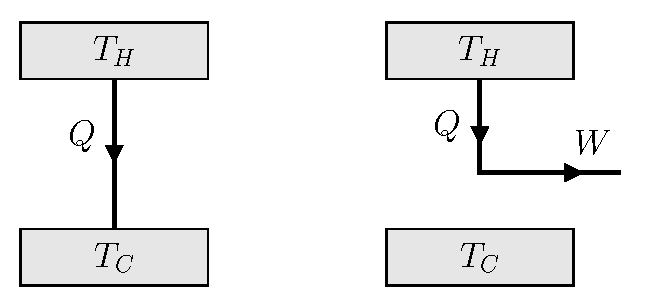
\includegraphics[width=2.7in]{heat_engines/impossible.eps}
\caption{On the left, heat flows from a hot reservoir at temperature $T_H$
  to a cold reservoir at $T_C$.  On the right, how the diagram would
  be altered if we could convert the heat $Q$ into work $W$.}
\label{fig:impossible_engine}
\end{center}
\end{figure}

Can we simply convert all the heat to work?  The first law of
thermodynamics, a.k.a. energy conservation, would have no problem with
this.  This hypothetical engine is illustrated in
Fig.~\ref{fig:impossible_engine}.  In both scenarios in this figure,
the hot reservoir is giving off heat $Q$, and so has negative entropy
change.  Since we are dealing with a reservoir, we use the 
constant temperature approximation (Eq.~\ref{eq:deltaS_isothermal}) to find
\begin{equation}
\Delta S_H = -\frac{|Q|}{T_H}.
\end{equation}
(We use absolute value bars so that there no confusion about the sign
of $Q$).  For the figure on the left, this negative entropy change is
allowed, because it is offset by the positive entropy change of the
cold reservoir, $\Delta S_C=|Q|/T_C$.  But for the figure on the
right, there is no compensating positive entropy change.  And so if we
could convert all heat to work, then
\begin{equation}
\Delta S_\text{total} = \Delta S_H = -\frac{|Q|}{T_H} < 0
\end{equation}
which violates the second law!  So we cannot do this.

But, you may have noticed that we could still satisfy the second law in
the previous example even if we didn't dump all of the heat $Q$ into the
cold reservoir.  Suppose we only dumped enough heat to make the positive
$\Delta S_C$ large enough to compensate for the negative $\Delta S_H$.
That would leave a little energy that we could conceivably convert to
work, while satisfying the second law (and the first, for that matter).

A schematic diagram of this process --- called an {\it engine diagram}
--- is shown in Fig.~\ref{fig:engine_diagram}.  An amount of heat
$Q_H$ is pulled from the hot reservoir, and an amount $Q_C$ is dumped
into the cold reservoir.  In between, some device which we'll call the
working substance intercepts this heat and produces work.  For now,
don't worry about how this might actually be accomplished; we'll
discuss that in detail in the next section.  Instead, focus on the big
picture: such a device will be consistent with the first law as long
as we conserve energy.  Looking at the arrows for energy flow, this
tells us
\begin{equation}
|Q_H| = |Q_C| + |W|. \qquad\text{(first law)}
\end{equation}
Again, we have used absolute value bars everywhere to avoid ambiguity about
whether the symbol $Q_H$ represent the heat flow out of the hot
reservoir (in which case it is a negative value), or the heat flow in
to the work substance (in which case it is positive). 
% To avoid
%confusion, we will use explicit absolute value bars and put the signs
%in ``by hand.''

\begin{figure}
\begin{center}
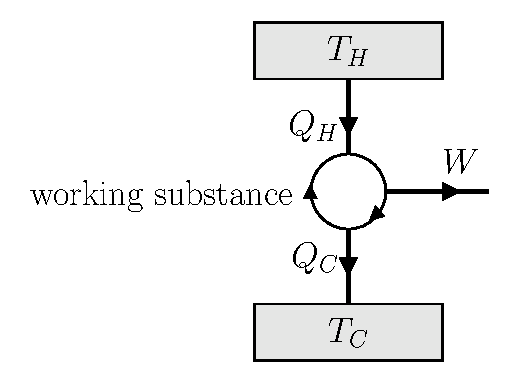
\includegraphics[width=2.4in]{heat_engines/engine_diagram.eps}
\caption{Engine diagram.}
\label{fig:engine_diagram}
\end{center}
\end{figure}

And continuing with the big picture: such a device will be consistent
with the second law as long as the total entropy doesn't decrease.  So
where do entropy changes happen?  Certainly in the reservoirs.  The
hot reservoir has an entropy decrease (since heat leaves the
reservoir) and the cold reservoir has an entropy increase 
(since heat is added to the reservoir).  But what about the 
working substance?  This gets at an
essential point: in order to be a heat engine, the working substance is {\it
  not} a source of energy.  It's not a battery stuck in between the
reservoirs, or anything else consuming chemical energy.  Rather, it
must be returned back to the same state it started from, so the
process can be repeated indefinitely.  But if this is the case, if the
working substance undergoes some cyclic process, then we
can use Eq.~(\ref{eq:DeltaS_cyclic}), which tells us $\Delta
S_\text{w.s.}=0$, since the final and initial states are the same.

And now we can do the complete entropy accounting:
\begin{equation}
  \Delta S_\text{total}= \Delta S_H + \Delta S_C + 
  \cancelto{0}{\Delta S}_\text{w.s.}
  = -\frac{|Q_H|}{T_H}+ \frac{|Q_C|}{T_C}  \geq 0 \quad\text{(second
    law)}
\label{eq:engine_second_law}
\end{equation}

One way to think of Eq.~(\ref{eq:engine_second_law}) is that it gives
a lower bound on how much heat we have to dump to the cold reservoir:
\begin{equation}
|Q_C| \geq \frac{T_C}{T_H}|Q_H|.
\end{equation}
That lower bound isn't zero, so we must dump some heat.
{\it This is an important result\/}:  any heat engine {\it must\/}
dump some of its heat into a cold reservoir.  It is impossible
to turn all heat into usable mechanical energy. 

But the good news is that the lower bound on the dumped heat $|Q_C|$
is smaller than $|Q_H|$, so we do get to ``skim off'' some of the
energy and generate some work.  Notice that the bound on how much heat
we have to dump becomes smaller for very large $T_H$ or small $T_C$.
Evidently, the more extreme the difference in temperature between the
reservoir, the more work we will be able to extract.

Let's quantify that.  Let's introduce a dimensionless quantity called
the efficiency, which is simply the fraction of heat pulled out of the
hot reservoir that we are able to convert to work:
\begin{equation}
\epsilon \equiv \frac{|W|}{|Q_H|}.
\label{eq:efficiency_def}
\end{equation}
From the first law we know $|W|=|Q_H|-|Q_C|$, so we can substitute
this in and write the efficiency equivalently as
\begin{equation}
\epsilon = \frac{|Q_H|-|Q_C|}{|Q_H|} = 1 - \frac{|Q_C|}{|Q_H|}.
\label{eq:general_efficiency}
\end{equation}
Obviously, the efficiency can't ever be greater than 1;
that would correspond to an engine that produces more mechanical energy
than the amount of heat that flows into it, and that would violate the
first law of thermodynamics.  But since $|Q_C|$ can never be zero in
a real engine --- we must always dump some heat --- the efficiency can
never reach 1.   That would violate the second law of thermodynamics.
We'll say more about this in a bit, after we have done a simple example
using efficiency.

\begin{example}{A simple engine problem}
\label{ex:simple_engine}

\begin{figure}[b]
\begin{center}
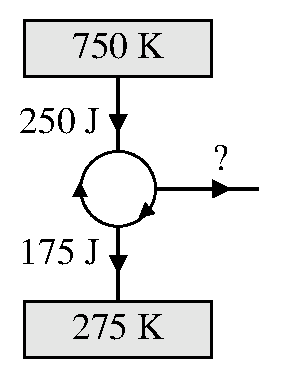
\includegraphics[width=1.1in]{heat_engines/engine_for_example.eps}
\caption{Diagram for Example \ref{ex:simple_engine}}
\label{fig:engine_for_example}
\end{center}
\end{figure}
An engine is described by the engine diagram in
Fig.~\ref{fig:engine_for_example}.  Determine the work output by this
engine and the efficiency of the engine.

\solution
%We could get the answer from Eq.~(\ref{eq:general_efficiency}), but
%we really don't need that. 
We can straightforwardly find the work done
by this engine using the first law of thermodynamics, i.e., energy
conservation.  The energy going into the working substance is
equal to the energy going out of the working substance, so
\begin{equation}
|Q_H| = |Q_C| + |W|
\end{equation}
and
\begin{equation}
|W| = |Q_H| - |Q_C| = 250\units{J} - 175\units{J} = 75\units{J} .
\end{equation}
Then from the definition of efficiency, Eq.~(\ref{eq:efficiency_def}),
we have
\begin{equation*}
\epsilon = \frac{|W|}{|Q_H|}  = \frac{75\units{J}}{250\units{J}} = \boxed{0.30}.
\end{equation*}
\end{example}

Okay, so we have a definition for efficiency, which can never be
greater than one (that would violate the first law of thermodynamics).
But it can never {\bf be equal to} 1 either.\footnote{This is
  important: if you ever calculate an efficiency equal to or greater
  than one, then it is wrong.}  The maximum value of $\epsilon$
corresponds to $|Q_C|$ being at its minimum (since it is being subtracted).
Evidently,
\begin{equation}
\epsilon_\text{max} = 1 - \frac{|Q_{C,{\rm min}}|}{|Q_H|} = 1 -
\frac{(T_C/T_H)|Q_H|}{|Q_H|} = 1-\frac{T_C}{T_H}.
\label{eq:max_efficiency}
\end{equation}
Warning: do not confuse this result for the maximum efficiency
$\epsilon_\text{max}$ with the similar looking expression
Eq.~(\ref{eq:general_efficiency}) for efficiency $\epsilon$ in general.
% Added following in 2010 to keep students from thinking this is
% general
Also, this is only valid if heat is drawn from and dumped into 
isothermal reservoirs.

It is worth keeping in mind that Eq.~(\ref{eq:max_efficiency}) for the
maximum efficiency is really a special case of an engine operating
between two thermal reservoirs.  A more general approach is just to
use the first and second laws of thermodynamics.  The first law just says
balance the energy in and the energy out, and the second law says
% In fact, using the
%first and second laws is preferable, because
%Eq.~(\ref{eq:max_efficiency}) only works if the engine operates
%between two thermal reservoirs.  This approach 
%
%will work for both
%simple reservoir problems and more complicated problems as well.
\begin{equation}
\Delta S_\text{total} = 0 \qquad\text{(maximum efficiency)}
\end{equation}
Ultimately, that's the one equation you need to remember
to solve problems involving a maximally efficient engine.

Let's consider some examples:
\newpage

\begin{example}{Automobile Efficiency}

\label{example:automobile_efficiency}

The internal combustion engine of an automobile is a heat engine.
Yes, there is gas being consumed, but that's being burned to provide
the high temperature of the hot reservoir.  From there on, the engine
functions as a heat engine.  

The hot reservoir is about $820^\circ\units{C}$ and the cold reservoir
is almost air temperature, but typically more like
$70^\circ\units{C}$.  Burning a gallon of gasoline provides about
$120\units{MJ}$ of heat.  What is the upper limit on how much work can
be extracted from a gallon of gas, and how much heat must be dumped?

\solution The moment you see the words ``upper limit'' (or similar
language), then you can pull out the second law of thermodynamics:
$\Delta S_\text{total} = 0$.  For this problem, $\Delta S_\text{total}
= \Delta S_H + \Delta S_C$, since the reservoirs are the
only parts of this system whose entropy changes.

To calculate $\Delta S$ for the reservoirs, we need to convert the
temperatures to Kelvin, so $T_H=820+273=1093\units{K}$ and
$T_C=70+273=343\units{K}$.  The entropy change of the hot reservoir is
\begin{equation}
\Delta S_H = \frac{-|Q_H|}{T_H} = 
-\frac{120\times 10^6\units{J}}{1093\units{K}}
 = -1.10\times 10^{5}\units{J/K}
\end{equation}
Therefore, since $\Delta S_\text{total} = 0$, it follows that  
$\Delta S_C$ must be positive by at least this amount.
\begin{equation}
\Delta S_{C,{\rm min}} = \frac{|Q_{C,{\rm min}}|}{T_C} = 1.10\times
10^5\units{J/K}
\end{equation}
so
\begin{equation}
|Q_{C,{\rm min}}| = 343\units{K} \cdot 1.10\times 10^{5}\units{J/K} =
\boxed{37.7\units{MJ}.}
\end{equation}
We get the maximum work by subtracting this from $|Q_H|$:
\begin{equation}
|W_\text{max}| = 120 - 37.7 = \boxed{82\units{MJ}.}
\end{equation}
In reality, the work output is only about 1/3 of this amount, due to
(i) design choices to get the work out faster, i.e. to get more power,
(ii) friction, and (iii) imperfect combustion of the fuel.
\end{example}

We could have solved the previous example by using the equation for
$\epsilon_\text{max}$ for engines with thermal reservoirs (although 
there was no need to do so).  The following is an example where 
the $\epsilon_\text{max}$ approach would not work; i.e., you
{\bf must} start from the second law of thermodynamics:
\begin{example}{A Two-Brick Heat Engine}
  \label{example:two_brick_heat_engine}
  A hot brick initially at temperature $T_H=400\units{K}$ is used as
  the source for a heat engine.  An equal sized cold brick made of the
  same material, initially at temperature $T_C=300\units{K}$, is used
  to dump the waste heat.  As the heat flows, the two bricks come to
  thermal equilibrium.  Assuming the heat engine was maximally
  efficient, what is the final temperature?

  \solution You might think the final temperature should just be
  $350\units{K}$, but that would be true only if we didn't intercept
  any of the heat and convert it to work.

  There is a lot we aren't given.  We don't know the amounts
  or the composition of the bricks, but we know they are identical.
  The hotter brick is going to cool from $400\units{K}$ down to some
  $T_f$, so its entropy change will be $\Delta S_H = nC\ln(T_f/400)$,
  which is negative since $T_f/400<1$.  The colder brick will warm
  from $300\units{K}$ to $T_f$, so its entropy change will be $\Delta
  S_C=nC\ln(T_f/300)$.  For maximum efficiency, then,
\begin{equation}
\Delta S_\text{total} = \Delta S_H+ \Delta S_C =
nC\ln\left(\frac{T_f}{400}\right) + nC\ln\left(\frac{T_f}{300}\right)
= 0.
\end{equation}
The $nC$ factors divide out, and we get
\begin{equation}
  \ln T_f - \ln 400 + \ln T_f - \ln 300 = 0
%\ln\left(\frac{T_f}{400}\right) =-\ln\left(\frac{T_f}{300}\right)
% = \ln\left(\frac{300}{T_f}\right)
\end{equation}
and so
\begin{eqnarray}
2\ln T_f = \ln(400\cdot 300) \quad&\Rightarrow&\quad 
%\frac{T_f}{400}= \frac{300}{T_f} \quad\Rightarrow\quad
T_f^2=400\cdot 300  \nonumber \\ 
      &\Rightarrow&\quad \boxed{T_f = 346.4\units{K}.} 
\end{eqnarray}
We see that the bricks end up slightly cooler than $350\units{K}$,
which makes sense since we skimmed off some of the energy as it was
flowing from hot to cold.
\end{example}

\section{Gas Cycles for Heat Engines}

We have made the case that skimming off some heat flow and generating
work is possible, that is, consistent with energy conservation and the
second law.  But how do we actually make a heat engine?  We need to
find some working substance that can take in heat, do work, and dump
heat.  We do not have to look very far: an ideal gas will do the job
nicely.  In fact, gases are the most commonly used substance in heat
engines today.

Consider a gas enclosed in a cylinder with a movable piston, as shown
in Fig.~\ref{fig:gas_piston}.  Recall that the work done by a gas is
given by
\begin{equation}
W_\text{by} = \int_A^B p\,dV,
\end{equation}  
so the gas can do work if we let the piston expand.  We can put heat
into the gas by bringing it into contact with something at a higher
temperature, and we can dump heat out of the gas by bringing it into
contact with something at a lower temperature.  To be useful, we will
want to complete a full cycle, to bring the gas back to its starting
point.  This means contracting the piston at some point in the cycle,
which will cost work (i.e., work is done {\bf on} the piston, or
work done {\bf by} the piston is negative).   But part of the cycle
will involve an expansion, and that produces positive work by the
piston.  Overall, we can get work out of the process (i.e., the net 
work by the piston is positive) if the expansion
happens with higher pressure (so more force) than the contraction.

A typical cycle is illustrated in Fig.~\ref{fig:gas_piston}. Notice
that the expansion happens at higher pressure than the compression,
leading to a net work being done by the gas.  These gas cylinders are
often paired up, as in an automobile, so that the expansion of one
cylinder causes the compression of the other cylinder, with power left
to spare.

\begin{figure}
\begin{center}
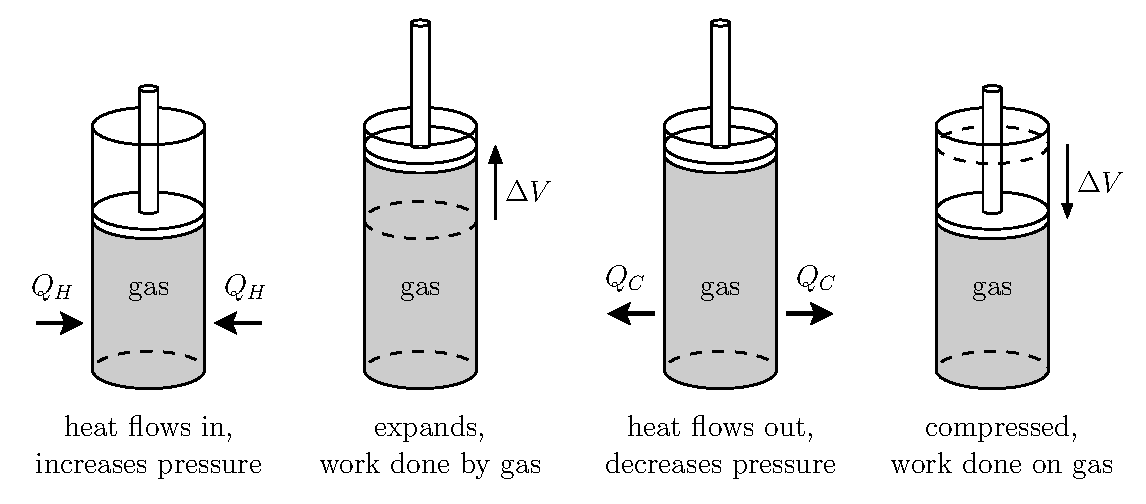
\includegraphics[width=5.5in]{heat_engines/gas_piston.eps}
\caption{Caption for gas-piston figure}
\label{fig:gas_piston}
\end{center}
\end{figure}

To quantify the cyclic gas process, it is useful to plot it on a
$p$\,-$V$ diagram.  One such cyclic process is illustrated in
Fig.~\ref{fig:rectangle_cycle}, which is a sequence of constant
pressure and constant volume processes that leads to a rectangular
cycle on the $p$\,-$V$ diagram.  Let's analyze this case in some detail,
starting with a calculation of the net work for the whole cycle.

\begin{figure}
\begin{center}
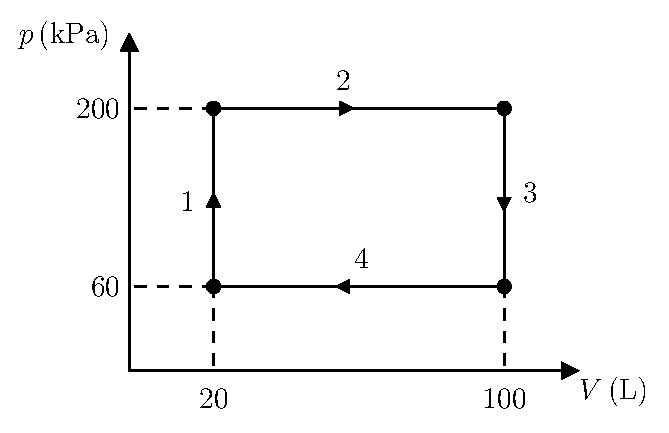
\includegraphics[width=3in]{heat_engines/rectangle.eps}
\caption{Cyclic process made up of constant pressure and constant volume
processes.}
\label{fig:rectangle_cycle}
\end{center}
\end{figure}

The constant volume steps do no work, while for constant pressure,
$W_\text{by}=p\Delta V$.  Adding this up around the whole cycle gives
\begin{align}
W_\text{cycle} &= W_1 +  W_2 + W_3 + W_4 \nonumber\\
 &= 0 + 200 \units{kPa}(+80\units{L}) + 0 +
 60\units{kPa}(-80\units{L})  = 140\cdot 80 \units{kPa$\cdot$L}\nonumber\\
&= 11.2\units{kJ}
\label{eq:work_for_rectangle}
\end{align}
Notice that the work done in the cycle is just the area of the enclosed
rectangle, which is true for any cycle.

Now let's figure out what $|Q_H|$ and $|Q_C|$ are.  For this we will
need to know whether the gas is monatomic or diatomic.  Let's assume
the gas is diatomic, so $f=5$ and $\gamma=1.4$.  For the constant
volume processes (steps 1 and 3 in Fig.~\ref{fig:rectangle_cycle})
there is no work done by the gas, so the first law says
\begin{equation}
 Q = \Delta E_\text{therm}+ 0 = {\textstyle\frac{5}{2}} \Delta(pV)
 = \textstyle{\frac{5}{2}} V\Delta p,
\end{equation}
where we've used the fact that $V$ is a constant in the last step.
Now we can calculate the heat flow into the gas for steps 1 and 3:
\begin{align}
Q_1 &= {\textstyle\frac{5}{2}}\cdot  20\units{L}\cdot (200\units{kPa}-60\units{kPa}) =
7.0\units{kJ}\nonumber\\
Q_3 &= {\textstyle\frac{5}{2}}\cdot  100\units{L} \cdot (60\units{kPa}-200\units{kPa}) =
-35.0\units{kJ}.
\end{align}
For a constant pressure process (steps 2 and 4 in
Fig.~\ref{fig:rectangle_cycle}) the work is $p\, \Delta V$ and so the
first law says
\begin{equation}
Q = \Delta E_\text{therm}+ W_\text{by} = {\textstyle\frac{5}{2}}\cdot \Delta(pV) +
p\Delta V = {\textstyle\frac{7}{2}}\cdot  p\Delta V.
\end{equation}
where we've used the fact that $p$ is a constant in the last step.
Now we can compute
\begin{align}
Q_2 &= {\textstyle\frac{7}{2}}\cdot  200\units{kPa}\cdot (100\units{L} - 20\units{L})
 = 56.0\units{kJ} \nonumber\\
Q_4 &= {\textstyle\frac{7}{2}}\cdot 60\units{kPa}\cdot (20\units{L} - 100\units{L})
 = -16.8\units{kJ} 
\end{align}
We have calculated the heat flow into the gas for each step.  Now we
can identify $Q_H$ as coming from all the steps with positive $Q$,
where heat really does flow in.  In our example, this would be steps 1
and 2.  In contrast, $Q_C$ comes from all the steps with negative $Q$,
where heat is actually flowing out of the gas, which is steps 3 and 4
for our example.  So we can calculate
\begin{align}
|Q_H| &= Q_1 + Q_2 = 7 + 56 = 63.0\units{kJ} \nonumber\\
|Q_C| &= |Q_3| + |Q_4| = 35 + 16.8 = 51.8\units{kJ}.
\end{align}
We can check our calculation, since we have already computed the work
in Eq.~(\ref{eq:work_for_rectangle}):
\begin{equation}
|W| = |Q_H|-|Q_C| = 63.0 - 51.8 = 11.2\units{kJ} \quad \surd
\end{equation}
And finally we can compute the efficiency,
\begin{equation}
\epsilon = \frac{|W|}{|Q_H|} = \frac{11.2}{63.0} = 0.178.
\end{equation}

This rectangular gas cycle engine is not actually practical.  Automobiles
use instead something called the Otto cycle, which is a sequence of
constant volume and adiabatic processes, as illustrated in
Fig.~\ref{fig:otto_cycle}.

\begin{figure}
\begin{center}
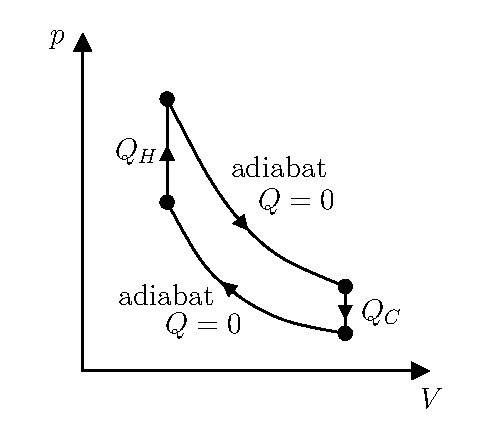
\includegraphics[width=2.5in]{heat_engines/otto_cycle.eps}
\caption{Otto cycle.}
\label{fig:otto_cycle}
\end{center}
\end{figure}

The heat for the constant volume steps is again given by
\begin{equation}
Q = \Delta E_\text{therm} = \frac{f}{2}V\Delta p \qquad\text{(constant
  volume)}
\end{equation}
which is positive when the pressure increases and negative when it
decreases.  And now for the nice part: by definition there is no heat flow during
either of the adiabatic steps, so these constant volume processes give
$Q_H$ and $Q_C$ as labeled in Fig.\ref{fig:otto_cycle}.  In the
homework problems you will work out the details of the Otto cycle.

The adiabats are exactly what makes this a more practical engine.
The adiabatic expansion and compression steps happen very quickly,
which is why no heat flows because it simply doesn't have enough time
to flow.  But this means a cycle is completed relatively quickly, and
so we are getting the work of the cycle out in a short amount of
time.  Recalling that work per time is power, we see that having a
fast cycle can lead to more power output, which is often desired.

\section{Refrigerators}

An interesting thing happens if we take a heat engine and run it
backwards: we make a refrigerator.  By refrigerator, we mean a device
which requires work as input and is able to make heat flow from a
colder object to a hotter object.  This includes, of course, the
refrigerator that keeps your milk from getting spoiled, but also
includes air conditioners and even heat pumps (which is basically an
air conditioner hooked up backwards to cool the outdoors and warm
your house).

Making heat flow from cold to hot may sound like a violation of
Clausius's statement of the second law, but it is not as long as
something else is going on in the process.  Heat will not
{\it spontaneously\/} flow from cold to hot; rather, we must cleverly
engineer the refrigerator to make it happen and, most importantly, we
must plug it in, to give the necessary work as input.

\begin{figure}
\begin{center}
\includegraphics[width=2in]{heat_engines/refrigerator_diagram.eps}
\caption{A refrigerator diagram, made by reversing all the arrows on a
  heat engine diagram.  Note that the working substance cycle is now
  counterclockwise instead of clockwise.}
\label{fig:refrigerator_diagram}
\end{center}
\end{figure}

Let's start with an engine diagram in reverse, as shown in
Fig.~\ref{fig:refrigerator_diagram}, and focus on the first and second
laws.  Energy conservation now requires
\begin{equation}
|Q_C| + |W| = |Q_H| \qquad\qquad\text{(first law)}
\end{equation}
which is exactly the same equation as before, since we reversed {\it
  all\/} the arrows.  Now the signs of the entropy change in the
reservoir are reversed, so the second law says
\begin{equation}
\Delta S_\text{total} = \Delta S_H + \Delta S_C = 
 \frac{|Q_H|}{T_H} - \frac{|Q_C|}{T_C} \geq 0.\quad\text{(second law)}
\end{equation}
 This now provides an {\it upper\/} bound on $|Q_C|$, namely
\begin{equation}
|Q_C| \leq \frac{T_C}{T_H}|Q_H|.
\label{eq:qc_upper_bound}
\end{equation}

What does this mean?  It means we can run a heat engine backwards and
satisfy the first and second laws and actually make some heat go from
cold to hot.  But there is a limitation on how much heat we can pull
out of the cold reservoir, and this limitation depends on the
reservoir temperatures and on how much work we provide.  If we
eliminate $|Q_H|$ from the upper bound, Eq.~(\ref{eq:qc_upper_bound}),
we can show
\begin{equation}
|Q_C| \leq \frac{T_C}{T_H-T_C} |W|,
\label{eq:qc_upper_bound_ii}
\end{equation}
which you will derive in the homework.  This expression says that we
need work to pull heat out of the cold reservoir, and also that the
effectiveness of pulling out heat will depend on the reservoir
temperatures.  We can quantify this ``effectiveness'' with what is
called the coefficient of performance, $CP$, defined as the ratio of
what want ($|Q_C|$) to what we must pay ($|W|$):
\begin{equation}
CP = \frac{|Q_C|}{|W|} \leq  \frac{T_C}{T_H-T_C}.
\end{equation}
As before, the maximum coefficient of performance is obtained from the
borderline case of the second law $\Delta S_\text{total}=0$.
Notice that reservoirs that are close in temperature yield a larger
$CP$.  This makes sense, since the closer $T_H$ and $T_C$ are, the
less ``uphill'' we are making the heat flow.

In the refrigerator diagram the working substance now goes
through a counterclockwise gas cycle.  This allows for the heat to
flow into the gas while it is at a lower temperature (lower than
$T_C$) and heat to flow out of the gas while it is at a higher
temperature (higher than $T_H$).  But this counterclockwise cycle also
means compression happens at higher pressure than the expansion.  This
will require some outside source of work to drive the gas through this
cycle, which is exactly what we found from general first law and
second law considerations: work input is necessary to make the
refrigerator function.  In other words, your refrigerator won't function
properly if you forget to plug it in.



\newpage

\section*{Problems}
\markright{PROBLEMS}

\begin{problem} 
  A $36\units{g}$ ice cube at $0^\circ\units{C}$ is dropped into
  $90\units{g}$ of water at $22^\circ\units{C}$.  Heat flows from the
  water to the ice, bringing both to equilibrium at
  $0^\circ\units{C}$.
  \begin{enumerate}
  \item Determine the number of moles of ice melted in cooling the
    water to $0^\circ\units{C}$.
  \item Calculate the entropy change of the melted ice.
  \item Calculate the entropy change of the $90\units{g}$ of water 
   in this process.  Is your answer consistent
    with the second law?
  \end{enumerate}
\label{prob:iceintowater}
\end{problem}

\begin{problem}
  Consider a pair of $5.0\units{mol}$ ideal solids.  Solid $A$ initially has
  a temperature of $500\units{K}$, while solid $B$ has a temperature of
  $200\units{K}$.  The solids are brought into thermal contact, and
% Added in 2010.
  heat flows until the system reaches equilibrium.
  Determine the entropy change of each solid, and the total entropy
  change. 
\end{problem}

\begin{problem}
  By what factor is the multiplicity increased in melting
  $18\units{g}$ of $0^\circ\units{C}$ ice into $0^\circ\units{C}$ water?
\label{prob:multiplicityformelting}
\end{problem}

\begin{problem} 
% an assigned problem to make the point that eps \neq eps_max
  A heat engine draws $600\units{J}$ of heat per cycle from a hot
  reservoir at $800\units{K}$, and dumps $300\units{J}$ of heat per
  cycle into a cold reservoir at $200\units{K}$.  Determine the
  efficiency of this engine.
\label{prob:simpleengine}
\end{problem}

\begin{problem}
  Consider a $10\units{mol}$  brick of ideal solid initially at temperature
  $500\units{K}$.  This brick is used as the heat source for a heat
  engine, which is dumping heat to a room-temperature reservoir at
  $295\units{K}$.
  \begin{enumerate}
  \item Determine the entropy change of the brick as it cools to room
    temperature.
  \item Determine the minimum amount of heat that must be dumped by
    this heat engine.
  \item Calculate the efficiency of this best-case engine.
  \end{enumerate}
\label{prob:onebrickengine}
\end{problem}

\begin{problem} 
  Consider the two-brick heat engine of
  Example~\ref{example:two_brick_heat_engine}.  Calculate the maximum
  amount of work that could be obtained from this engine.  For this
  problem, assume that the bricks are each an ideal solid with 
  $2.0\units{mol}$.  
\label{prob:twobrickengine}
\end{problem}
\newpage

\begin{problem} 
  Susquehanna Valley Limousine has modified their automobile engine to
  provide heat for an oven to bake fresh chocolate chip cookies while
  you cruise Lewisburg.\footnote{Not really.}  For each gallon of gas,
  $12\units{MJ}$ of heat is dumped from the engine into the oven at a 
  temperature of $190^\circ\units{C}$, and the remainder of the heat 
  coming from the engine is dumped to the environment at 
  $70^\circ\units{C}$, as described in 
  Example~\ref{example:automobile_efficiency}.  Calculate the maximum
  work possible from a gallon of gas for this engine.  As in 
  Example~\ref{example:automobile_efficiency}, assume that the hot
  reservoir has a temperature of $820^{\circ}\units{C}$ and the 
  heat coming from the burning gas totals $120\units{MJ}$.
  \begin{figure}[h]
   \begin{center}
   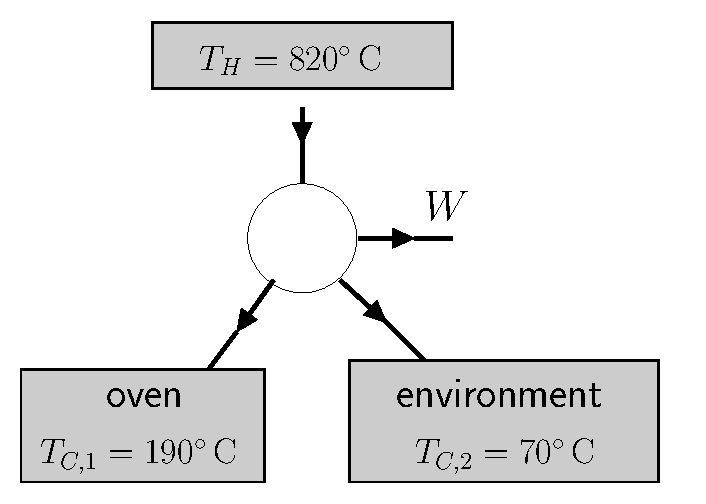
\includegraphics[width=3.0in]{heat_engines/limousine.eps} 
   \end{center} 
   \caption{Engine diagram for Problem \ref{prob:limousine}}
   \end{figure}
\label{prob:limousine} 
\end{problem}
\newpage

\begin{problem}  % A55, brought into chapter
  In the cycle shown below, $1.0\units{mol}$  of a
  monatomic ideal gas is initially at a pressure of $p_A=100\units{kPa}$
  and a temperature of $T_A=0^\circ\units{C}$.  The gas is heated at
  constant volume to $T_B = 150^\circ\units{C}$ and is then expanded
  adiabatically until its pressure is back to $p_C=100\units{kPa}$.
  Finally, the gas is compressed at constant pressure until it is back
  to its original state $A$.  Find
  \begin{enumerate}
  \item the pressure, volume and temperature for each of the three
  labeled points (A, B and C),
  \item the heat entering or leaving the system during each process, and
  \item the efficiency of this cycle.
  \end{enumerate}
  \begin{figure}[h]
    \begin{center}
      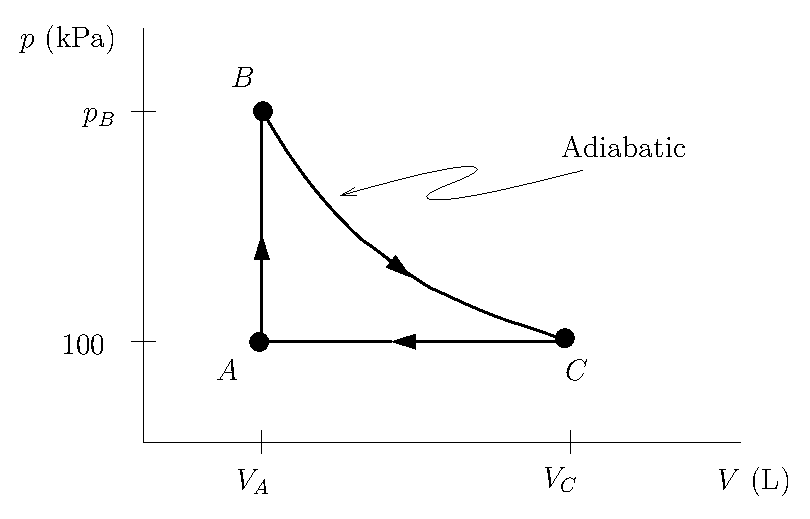
\includegraphics[width=3.5in]{heat_engines/cycle.eps}
    \end{center}
    \caption{Cycle for Problem \ref{prob:threelegcycle}} 
  \end{figure}
\label{prob:threelegcycle}
\end{problem}

\begin{problem} 
  For the rectangular gas cycle in Fig.~\ref{fig:rectangle_cycle},
  assume that there is $0.50\units{mol}$ of diatomic gas.
  \begin{enumerate}
  \item If this cycle is to operate between two reservoirs, calculate
    the minimum possible value for $T_H$ and the maximum value for
    $T_C$.
  \item Compare the efficiency of this gas cycle to the maximum
    efficiency possible for a cycle operating between these two
    reservoirs.
  \end{enumerate}
\label{prob:rectangularcycle}
\end{problem}

\begin{problem} 
  Explain why, for any gas cycle that is clockwise on a $p$\,-$V$
  diagram, the area enclosed by the loop gives the net work by the gas
  in the cycle.
\end{problem}

\begin{problem} 
  Your problem session instructor will provide this problem.
%  Is an automobile engine more efficient in the summer or the 
%  winter?
%  Explain using general entropy/heat engine arguments, and also with a
%  $p$\,-$V$ diagram. (Note:  overall gas mileage for a car also depends
%  quite strongly on tire pressure, which can also vary between the summer
%  and winter.)  Assume that the temperature to which the hot gasoline vapors
%are raised during  combustion  is unchanged.
\end{problem}

\begin{problem} 
  An Otto cycle for a fixed number of moles of a diatomic ideal gas is shown in
  Fig.~\ref{fig:otto_cycle_hw}. 
  \begin{figure}[h]
    \begin{center}
      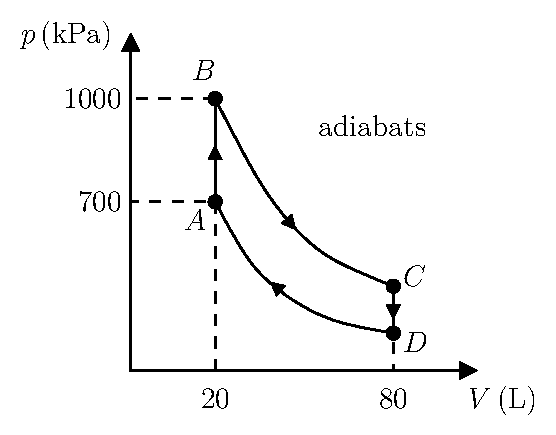
\includegraphics[width=3in]{heat_engines/otto_cycle_hw.eps}
      \caption{Otto cycle for Problem~\ref{prob:otto_cycle}.}
      \label{fig:otto_cycle_hw}
    \end{center}
  \end{figure}
   \begin{enumerate}
   \item Calculate the pressure at points $C$ and $D$.
   \item Determine $|Q_C|$, $|Q_H|$, and $|W|$ for one cycle.  {\it
       Hint:} save $|W|$ for last.
   \item Calculate efficiency of this cycle. 
   \end{enumerate}
   \label{prob:otto_cycle}
\end{problem}

% \begin{problem} {\bf Maximally efficient engine.} [in development]
%  Consider the following gas cycle: (i) isothermal expansion at
%  temperature $T_H$, (ii) adiabatic expansion until the gas cools to
%  $T_C$, (iii) isothermal compression at temperature $T_C$, and (iv)
%  adiabatic compression until the gas temperature reaches $T_H$.
%  Calculate $\epsilon$, compare to $\epsilon_\text{max}$.  Called
%  Carnot engine.  (b) why is this ideal?  Isotherms: heat flow between
%  (nearly) identical temperature reservoir and gas, (nearly) zero
%  entropy produced.  Adiabats: no heat flow, no entropy change.  Needs
%  work.
% \end{problem}

\begin{problem} 
  Derive Eq.~(\ref{eq:qc_upper_bound_ii}), the upper bound for $|Q_C|$
  in a refrigerator, by starting from the first and second laws.
\end{problem}

\begin{problem}
  Can you cool off your house by opening the door to the refrigerator?
  Explain why or why not.
\end{problem}


\begin{problem} 
 A  refrigerator is designed to  keep its interior  at a constant
  $5^\circ\units{C}$  while  dumping  heat  into  a  room  temperature
  environment at $22^\circ\units{C}$.  The interior of
  the refrigerator may be regarded as a cold reservoir, 
while the air  around it is a
  hot reservoir.  Now suppose  a pitcher containing $1800\units{g}$ of
  room-temperature water  is put into  the refrigerator. We  can break
  down what happens next into two  steps: (1) the water will cool down
  to the  temperature of the  cold reservoir (fridge interior)  as its
  heat flows into  cold reservoir, and (2) the  refrigerator will turn
  on and do  work (run a compressor, circulate  refrigerant, etc.)  to
  extract this  heat from  the cold  interior and dump  it to  the air
  outside.

We'll calculate what happens in each of these steps.

Step \#1:
\begin{enumerate}
\item  Calculate the change in entropy of the water as it cools from 
$22^\circ\units{C}$ to $5^\circ\units{C}$.
\item Calculate the change in entropy of the cold reservoir (i.e. the
inside of the refrigerator) due to this same heat transfer.

\item Is the second law of thermodynamics satisfied in this step?
Explain briefly why or why not, using your results above.
\end{enumerate}

Step \#2
\begin{enumerate}

\item Now we must get rid of the extra heat in the cold reservoir 
  by   transferring  it  to  the  hot  reservoir.
  Calculate the change in the entropy of the cold reservoir
(refrigerator) as the excess heat
  from step \#1 is removed from the refrigerator's interior.

\item  Determine the minimum amount  of work required to remove this 
excess heat
from the cold reservoir. 

% \item  Optional: Is this two-step refrigerator maximally efficient in cooling
% the water?  If so, how do you know? If not, can you think of a way to make it more efficient?

\end{enumerate}
\end{problem}


% \begin{problem} 
%   A refrigerator is designed to dump heat into a room temperature
%   environment at $22^\circ\units{C}$ while keeping the interior at  
%   $5^\circ\units{C}$.   In this problem, you may treat the interior 
%   of the refrigerator as a cold reservoir.  If you put pitcher containing
%   $1800\units{g}$ of room temperature water into to the refrigerator, it 
%   will cool down to the temperature of the interior reservoir, dumping 
%   heat into the cold reservoir.  What is the minimum amount of work 
%   required to remove this heat from the interior of the refrigerator.
% \end{problem}

% \begin{problem} 
%  Hard (do we want this?): rectangle pV diagram: why can't this be a
%  refrigerator?  Hint: think about where on the cycle $Q_h$ and $Q_C$
%  occurs, and what the temperature of the working substance (the gas)
%  is at that point in the pV diagram.  Is there any similar
%  restriction on heat engines?  I.e. some pV cycles that can't be heat
%  engines?
% \end{problem}


\chapter{Gravity and Geometry}
\label{chapter:gravity}

\section{Introduction}

Previously we have described the force of gravity on an object by a
field model.  In this Newtonian model, masses cause gravitational fields and
these fields act on other masses to cause forces.
    
In this chapter we examine another model of gravity which is
Einstein's explanation in terms of curved spacetime.  In this model
masses cause spacetime to be curved and other masses, moving in
`straight' lines in this curved spacetime, seem to accelerate relative
to the source mass.  As described succinctly by John A. Wheeler,
the leading spokesman for Einstein's theory of gravity: 

\begin{quote}
Mass tells spacetime how to curve;  spacetime tells mass how to
move.
\end{quote}

We begin by looking again at the concept of the invariant spacetime
interval.  We present the modifications of the interval that Einstein
introduced to account for the effects of gravity.  This leads us to
examine how the gravitational effects of a spherical mass (like
planets and stars) show up in clock rates and the measurement of
distances.
    
We also develop the idea of curved space and describe how one might
determine whether the three-dimensional space we live in is curved.
We apply this idea to the curvature of spacetime to examine how a
particle moves in curved spacetime and present an unusual principle
called the principle of maximum proper time which governs how an
object moves in the presence of a gravitational field.

\section{The Interval Revisited}

In developing his conception of gravity as a manifestation of curved
spacetime, Einstein sought to extend his notion of invariance from
special relativity.  Recall that for special relativity all
\textit{inertial} reference frames were treated as equally valid for
describing physics.  In 1915, Einstein created the theory of general
relativity, removing the inertial frame restriction: \textit{all
  arbitrarily} moving reference frames were to be equally valid.  This
enabled him to include gravity into spacetime physics.

Recall that in Sec.~\ref{sec:spacetime_intervals} we introduced the
spacetime interval $I^2$ of special relativity, defined by
\begin{equation}
I^2 = (c\Delta t)^2 - (\Delta x)^2.
\end{equation}     
The interval was shown to be invariant: observers in any inertial
reference frame would calculate the same value for the interval
separating any given pair of events.

\begin{figure}[tbp]
\begin{center}
\includegraphics[width=2.5in]{gravity_and_geometry/coordinates.pdf}
\end{center}
\caption{Cartesian to polar coordinates}
\label{fig:cartesian_to_spherical}
\end{figure}

Let's work on generalizing this expression to include the effects of
gravity.  The first thing to do is convert from Cartesian to polar
coordinates, shown in Fig.~\ref{fig:cartesian_to_spherical}, as
these will be more appropriate to describe spacetime in the presence
of spherically symmetric masses, like Earth, stars, or black holes.
Here ``$r$'' is a radial coordinate: it decreases or increases as you
move toward or away from the given spherical mass.  The interval
expressed in these coordinates, not surprisingly, takes the form
\begin{equation}
I^2 =  (c\Delta t)^2 - \Delta r^2
\label{eq:flat_space_spherical}
\end{equation}
when motion along only the radial direction is considered.

Next, let's see how Einstein includes the effects of gravity in the
invariant spacetime interval.  How is it that ``mass tells spacetime
how to curve''?  The full answer is very hard, far beyond the scope of
this course: solve a set of nasty coupled nonlinear differential
equations!  But for the case of intervals in the spacetime outside a
spherical mass, the result is surprisingly simple.
Eq.~(\ref{eq:flat_space_spherical}) becomes
\begin{equation}
  I^2 = \biggl(1-\frac{2GM}{c^2 r}\biggr)(c\Delta t)^2-
  \biggl(1-\frac{2GM}{c^2 r}\biggr)^{-1}\Delta r^2. 
\label{eq:schwarzschild_metric}
\end{equation}
Here ``$M$'' is the mass of the central body, and $G$ is Newton's
universal gravitation constant.

The appearance of the coefficients $(1-\frac{2GM}{c^2r})$ and
$(1-\frac{2GM}{c^2r})^{-1}$ in the general relativistic expression for
the spacetime interval tells you that we're now dealing with curved
spacetime.  The presence of a nearby mass curves spacetime!  

Finally, recall from Sec.~\ref{sec:spacetime_intervals} that when
$I^2$ is positive the interval $I$ is timelike. In fact, the quantity
$I/c$ represents the proper time interval $\Delta\tau$ between the two
given events.  Dividing Eq.~(\ref{eq:schwarzschild_metric}) by $c^2$
and replacing $I/c$ with $\Delta\tau$, we get
\begin{equation}   
 \Delta\tau^2 = \biggl(1-\frac{2GM}{r}\biggr)\Delta t^2 - 
  \frac{1}{c^2}\biggl(1-\frac{2GM}{r}\biggr)^{-1}\Delta r^2.
\label{eq:curved_space_proper_time}
\end{equation}
On the other hand, when $I^2$ is negative, we are dealing with a
spacelike interval.  It is convenient to introduce $\Delta s$, the
proper distance, by 
\begin{equation}
 \Delta s^2 = -I^2 > 0.
\end{equation}
In this case, Eq.~(\ref{eq:schwarzschild_metric}) becomes
\begin{equation}
  \Delta s^2 =  \biggl(1-\frac{2GM}{r}\biggr)^{-1}\Delta r^2 -  
  \biggl(1-\frac{2GM}{r}\biggr)(c\Delta t)^2.
 \label{eq:curved_space_proper_distance}
\end{equation}
Let's explore how these gravity-related factors lead to the warping of
time and space.

\section{Gravity's Effect on Clock Rates}

An example will show how clock rates are affected by the curvature of
spacetime.  Consider two clocks, clock $A$ parked near a large mass,
and clock $B$ parked very far away.  Note that both clocks are at
rest: there is NO relative motion.  Yet general relativity predicts
that the clocks still run at different rates.

We start from Eq.~(\ref{eq:curved_space_proper_time})
\begin{equation}
  \Delta\tau^2 = \biggl(1-\frac{2GM}{c^2 r}\biggr)\Delta t^2-
  \frac{1}{c^2}\biggl(1-\frac{2GM}{c^2 r}\biggr)^{-1}\Delta r^2 
\label{eq:schwarzschild_metric_ii}
\end{equation}
and insert the conditions for clock $B$ and then for clock $A$.  For
clock $B$, it is at rest, so $\Delta r=0$.  Also it is very far away
(say $r\to\infty$), so that $\frac{2GM}{c^2r}\to 0$.  Then for $B$,
Eq.~(\ref{eq:schwarzschild_metric_ii}) becomes
\begin{equation}
  \Delta \tau_B^2 = (1-0)\Delta t^2 - \frac{1}{c^2} (1-0)^{-1} (0) = \Delta
  t^2 \quad\text{or}\quad \Delta\tau_B = \Delta\tau.
\end{equation}
This shows that $\Delta t$ is the proper time as recorded on far-away
clocks.

\begin{figure}[tbp]
\begin{center}
\includegraphics[width=1in]{gravity_and_geometry/clocks.pdf}
\end{center}
\caption{Low clocks are slow clocks!}
\label{fig:clocks}
\end{figure}

Now consider clock $A$, say at rest at radial location $r_A$.  Similar
to the above calculation we find
\begin{equation}
 \Delta\tau_A = \biggl( 1 - \frac{2GM}{c^2 r_A}\biggr)^{1/2} \Delta t
    = \biggl( 1 - \frac{2GM}{c^2 r_A}\biggr)^{1/2} \Delta\tau_B.
\label{eq:low_clock}
\end{equation}
Since $(1-\frac{2GM}{c^2r})^{1/2} < 1$, we see that
$\Delta\tau_A<\Delta\tau_B$.
This shows that clocks near a mass record \textit{less} elapsed proper
time than those far away.  As illustrated in Fig.~\ref{fig:clocks}, a
nice mnemonic is ``Low clocks are slow clocks''.

\begin{example}{Clocks on the Earth's Surface.}
How much slower does a clock at sea level run than one far away from
Earth?
\solution

Use Eq.~(\ref{eq:low_clock}), with $M=5.97\times 10^{24}\units{kg}$
and $r_A=R_E = 6.37\times 10^{6}\units{m}$
\begin{align}
 \Delta\tau_A &= \biggl(1-\frac{2\times 6.67\times 10^{-11}\times
   5.97\times 10^{24}}{(3.00\times 10^{8})^2 \times 6.37\times 10^{6}}
\biggr)^{1/2}\Delta\tau_B   \nonumber\\
   &= (1-1.39\times 10^{-9})^{1/2}\Delta\tau_B \nonumber\\
   &\approx (1 - 6.95\times 10^{-10}) \Delta\tau_B.
\end{align}
A useful way to express this result is the rate at which clock $A$
gets behind:
\begin{equation}
  \Delta\tau_B - \Delta\tau_A = \Delta\tau_B -
     (1 - 6.95\times 10^{-10}) \Delta\tau_B = 
6.95\times 10^{-10} \Delta\tau_B. 
\end{equation}
Thus clock $A$ falls behind clock $B$ an amount $6.95\times 10^{-10}$
seconds every second.  Thus, for clock $A$ to get behind clock $B$ by
one second, it takes 
\begin{equation}
\frac{1}{6.95\times 10^{-10}} \text{seconds} = 1.44\times
10^9\units{s}   \approx 46\units{yr}.
\end{equation}
\end{example}
We don't notice these time effects much near Earth, but these small
difference are essential to be accounted for in the design and
operations of GPS devices.  For a more dramatic example, see Problem
\ref{prob:neutron_star_time}.
 
\section{Curved Spacetime}
     
We now need to give a careful definition of the radial coordinate $r$.
We begin with an example in ordinary three-dimensional space.  Imagine
drawing two large circles on the earth with the north pole as the
common center (see Fig.~\ref{fig:sphere}).  Let $\Delta s$ be the distance
between one circle and the other, measured along the earth's surface
as we walk out from the north pole.  If we were sphere-dwellers who
lived entirely in 2-dimensions, that is, on the surface of the earth,
and knew nothing about a 3$^{\rm rd}$ dimension (up or down), we could
(having studied Euclidean geometry) {\em define} the radial
coordinates, $r_1$ and $r_2$, in terms of the circumferences of the
two circles, by
\begin{equation}
C_1 = 2\pi r_1\mbox{\hspace{.25in}and\hspace{.25in}}C_2 = 2\pi r_2.
\label{eq:circumference}
\end{equation}
The actual radii of the circles, $r_1$ and $r_2$, are shown in
Fig.~\ref{fig:sphere}; they clearly are not measured along the surface
of the earth.  But these radii are not available for direct
measurement by the sphere-dwellers; they must \textit{calculate} the
radii using Eq.~(\ref{eq:circumference}).
     
\begin{figure}[tbp]
\begin{center}
\includegraphics[width=2in]{gravity_and_geometry/sphere.eps}
\end{center}
\caption{Two concentric circles drawn on a sphere.}
\label{fig:sphere}
\end{figure}
     
If we lived on a flat space, such as a flat piece of paper, the radial
coordinates $r_1$ and $r_2$ would be related by
\begin{equation}
\Delta r = r_2 - r_1 = \Delta s \mbox{\hspace{0.5in}(flat space
  expectation)},
\label{eq:flat}
\end{equation}
where $\Delta s$ is the shortest distance between the circles measured
along the paper.  But when the circles are actually drawn on the
curved surface of the earth, $r_2$ is larger than $r_1$ by the amount
$\Delta r$, which is less than $\Delta s$.
     
We humans, who can comprehend the spherical nature of the earth's
surface, can understand this deviation from flat-space geometry by
studying Fig.~\ref{fig:sphere}, where the actual difference in radius,
$\Delta r$, between the two circles on the earth is clearly smaller
than $\Delta s$.  Thus, on a sphere, the flat-space expectation of
Eq.~(\ref{eq:flat}) is incorrect.  We can therefore use
Eq.~(\ref{eq:flat}) in an experimental test, performed entirely on the
surface of the earth, to determine whether that surface is curved or
flat.
     
The test requires that we measure the circumferences of the two
circles and the distance $\Delta s$ between them.  Then we must divide
each circumference by $2\pi$ to get the radial coordinate, substitute
these calculated values for $r_1$ and $r_2$, along with the measured
$\Delta s$, into Eq.~(\ref{eq:flat}) and check for equality.  If we
get equality then the surface is flat.  If $\Delta s$ is larger than
$r_2-r_1$, then the surface is curved like a sphere or a bowl.  (If
$\Delta s$ is smaller, the surface is curved like a saddle.)

\begin{figure}[tbp]
\begin{center}
\includegraphics[width=3.5in]{gravity_and_geometry/grav-photon.pdf}
\end{center}
\caption{An outward displacement $\Delta s$ in the gravitational field
  of a star.}
\label{fig:grav-photon}
\end{figure}
     
Now let's consider the region around a star as shown in
Fig.~\ref{fig:grav-photon}.  We ask whether the space around the star
is curved.  How can we tell?  We begin by drawing two circles centered
on the star, $C_1$ and $C_2$ in Fig.~\ref{fig:concentric}.  We then
measure their circumferences with meter sticks (which have been
properly calibrated with clocks and light pulses) and calculate $r_1$
and $r_2$.  We also measure the distance $\Delta s$, by laying meter
sticks radially along a path from $C_1$ to $C_2$.  Then to test
whether space is curved or flat, we substitute our measurements into
Eq.~(\ref{eq:flat}).  If Eq.~(\ref{eq:flat}) is satisfied, then space
is flat; otherwise it is curved.
         

\begin{figure}[t]
\begin{center}
\includegraphics[width=1.8in]{gravity_and_geometry/concentric.pdf}
\end{center}
\caption{Two concentric circles drawn around a star of mass $M$.}
\label{fig:concentric}
\end{figure}
     
When we do this experiment (say with radar ranging around the sun) we
find that actual measurements of phenomena occurring near the sun
indicate that $\Delta s$ is, in fact, slightly larger than $\Delta r$.
Thus Eq.~(\ref{eq:flat}) is {\em not} satisfied, and the space around
the sun is curved like a bowl.  The source of the curvature is the
mass $M$ of the sun.  It's like placing a large mass on a rubber
sheet; the added mass distorts and curves the sheet so that nearby
smaller masses are attracted to it.  Near a black hole, the curvature
effect is quite pronounced.  Figure~\ref{fig:curved-space} shows a
popular representation of the curved space near a black hole.
     
\begin{figure}[tbp]
\begin{center}
\includegraphics[width=4in]{gravity_and_geometry/black-hole.pdf}
\end{center}
\caption{Curved space near a black hole.  The distance $\Delta s$ measured
radially along the surface between circles of radial coordinate  $r_1$ 
and $r_2$ is larger than their  difference $\Delta r$.}
\label{fig:curved-space}
\end{figure}
     
Now imagine the motion of a small object in this curved space.  It
will try to follow the shortest path.  If it goes on a path that takes
it deep into the hole, where $\Delta s$ is much bigger than $\Delta
r$, the total distance will be larger than if the object skirts around
the hole, trading a lot of ``down-and-back-up'' distance for just a
little extra ``sideways'' distance.  This is why light bends around
large mass stars or galaxies (see
Fig.~\ref{fig:light-bent-by-curved-space}).

\begin{figure}[b]
\begin{center}
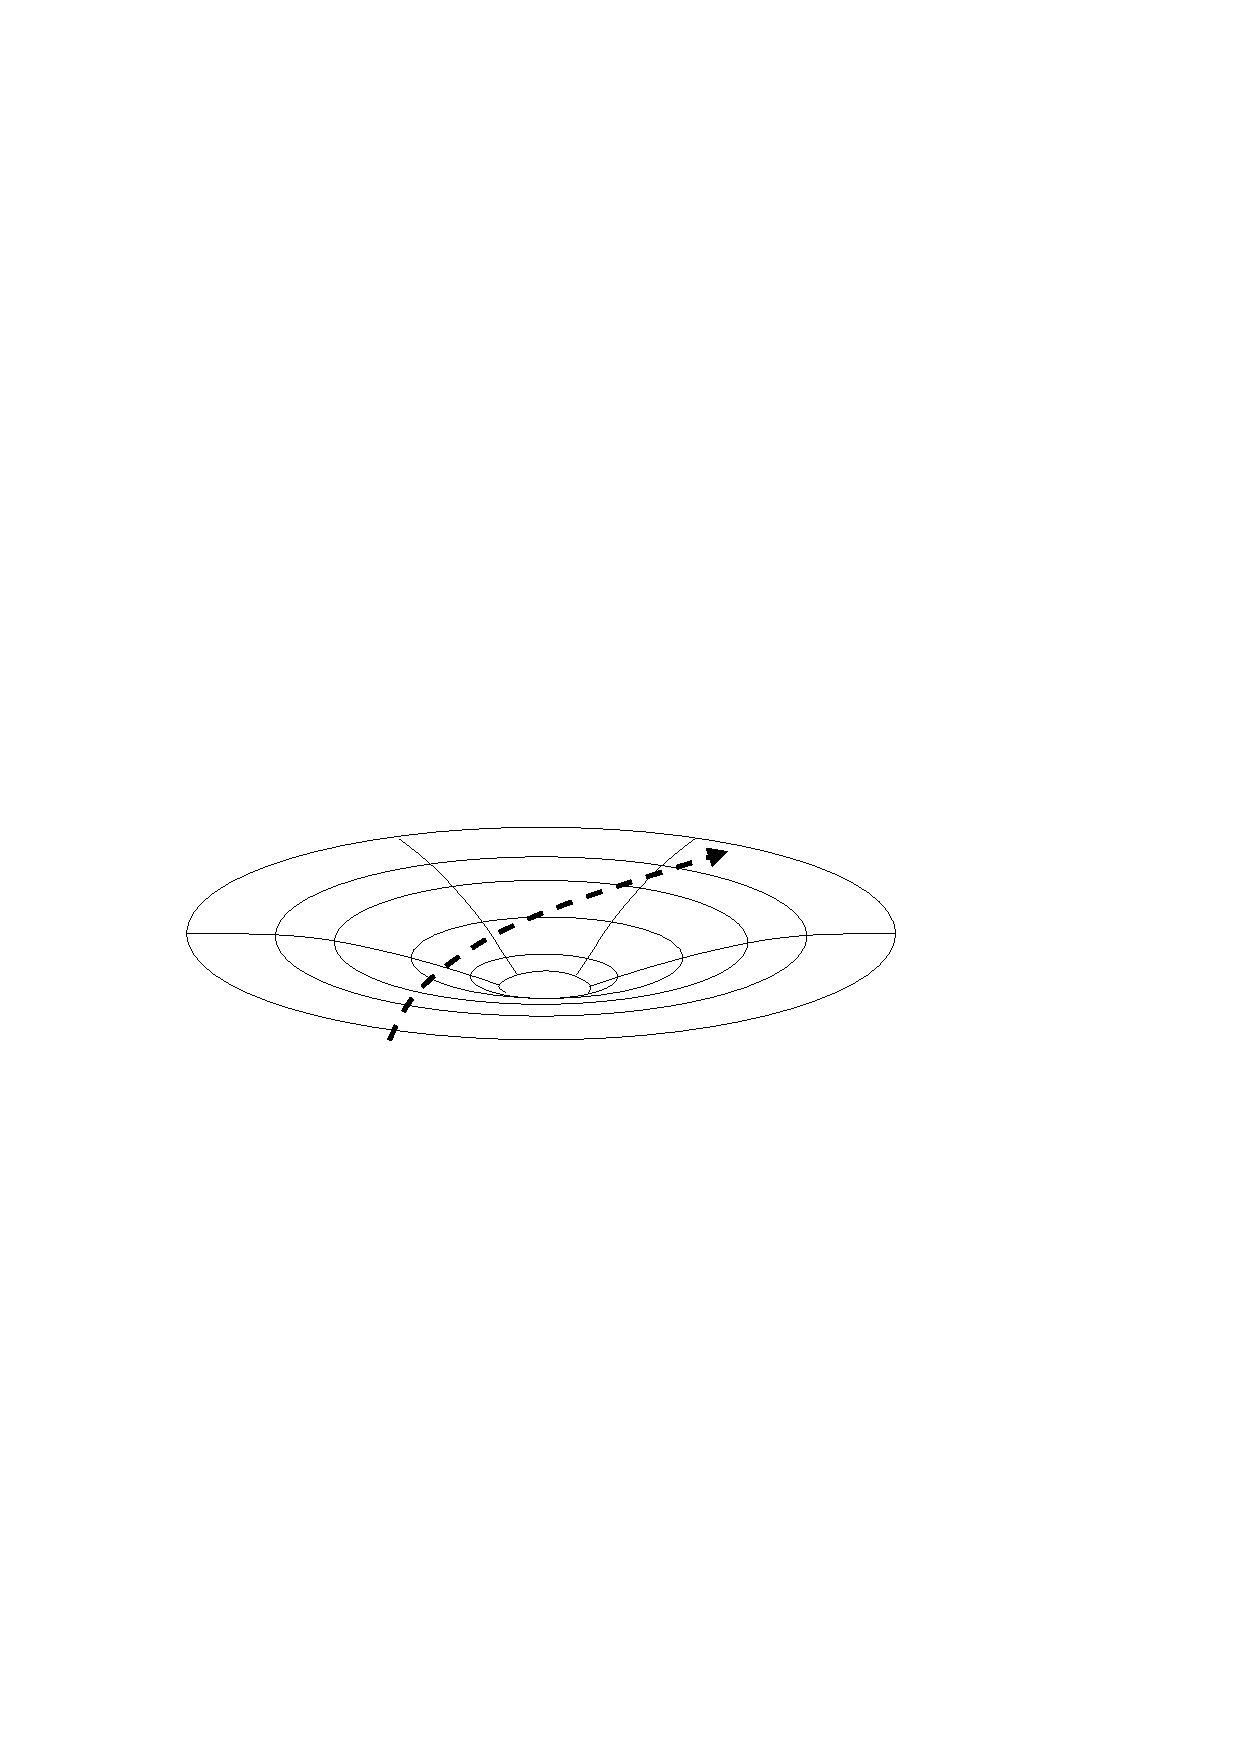
\includegraphics[width=3in]{gravity_and_geometry/black-hole-bends-light.pdf}
\end{center}
\caption{Light being bent by curved space near a black hole.}
\label{fig:light-bent-by-curved-space}
\end{figure}
     
It's time to get quantitative.  Can Einstein's conception of curved
spacetime near the sun tell us that $\Delta s$ is bigger than $\Delta
r$, and by how much?  Start with
Eq.~(\ref{eq:curved_space_proper_distance})
\begin{equation}
  \Delta s^2 =  \biggl(1-\frac{2GM}{r}\biggr)^{-1}\Delta r^2 -  
  \biggl(1-\frac{2GM}{r}\biggr)(c\Delta t)^2.
\end{equation}
%\begin{equation}
%  \frac{I^2}{c^2} = \Delta\tau^2 = 
%  \biggl(1-\frac{2GM}{c^2 r}\biggr)\Delta t^2-
%  \frac{1}{c^2}\biggl(1-\frac{2GM}{c^2 r}\biggr)^{-1}\Delta r^2. 
%\label{eq:schwarzschild_metric_iii}
%\end{equation}
%We need to convert this to  study the curvature of \textit{space}; the
%interval $I$ between points 1 and 2 is space-like, so $I^2<0$.  So
%let's write $I^2 = -\Delta s^2$, where $\Delta s$ is real and
%positive, the spatial separation.  Then
%Eq.~(\ref{eq:schwarzschild_metric_iii}) becomes
%\begin{equation}
%  -\frac{\Delta s^2}{c^2} =
%  \biggl(1-\frac{2GM}{c^2 r}\biggr)\Delta t^2-
%  \frac{1}{c^2}\biggl(1-\frac{2GM}{c^2 r}\biggr)^{-1}\Delta r^2. 
%\end{equation}
We would like to consider a snapshot of the space around the sun; that
is locate the two points at the \textit{same time}.  Thus set $\Delta
t=0$ and solve for $\Delta s$.  We find
\begin{equation}
  \Delta s = \biggl(1-\frac{2GM}{c^2 r}\biggr)^{-1/2}\Delta r.
\label{eq:schwarzschild_metric_iv}
\end{equation}
Since $(1-\frac{2GM}{c^2r})^{-1/2} > 1$ for any $M>0$ and $r<\infty$
we have that $\Delta s>\Delta r$ near any mass --- the space near
stars and planets is curved like a bowl!

\begin{example}{}
How curved is space near the sun?
\solution
Use Eq.~(\ref{eq:schwarzschild_metric_iv}) with $M=M_\text{sun}=
1.99\times 10^{30}\units{kg}$ and $r=R_\text{sun}=6.96\times
10^{8}\units{m}$.
\begin{align}
\Delta s &= \biggl(1-\frac{2\times 6.67\times 10^{-11}\times 1.99\times
  10^{30}}{(3.00\times 10^{8})^2\times 6.96\times
  10^8}\biggr)^{-1/2}\Delta r \nonumber\\
 &= (1-4.24\times 10^{-6})^{-1/2}\Delta r \nonumber\\
 &= 1.0000021\,\Delta r.
\end{align}
That's not looking very curved, but it is big enough to direct the
motion of all the planets in their orbits about the sun!
\end{example}


\section{Law of Motion for a Freely Falling Body}
     
Imagine taking a trip, in gravity-free spacetime, from the point $x =
0$, $t = 0$ to the point $x = 0$, $t = 1$.  Not a very adventurous
trip, to be sure, but some would opt for the lazy way; simply remain
at rest at $x = 0$ and you'll get there!  But there are other ways of
making the trip (see Fig.~\ref{fig:trip}).  For example you could take
off at some high speed, say $v = 0.6 c$ for half a second (in the rest
frame) and travel about 0.3\, light-sec and then suddenly reverse
direction and travel for another half second back to $x = 0$ at a
velocity of $-0.6 c$.  This hyperactive approach gets you to your
destination quicker, in the sense that the time elapsed on your watch
(proper time) will be only
\begin{equation}
\Delta t_{\rm proper} = \Delta t \sqrt{1 - v^2/c^2} = 
      1.0 \times \sqrt{1 - 0.6^2} = 0.8\, \mbox{s}. 
\label{eq:deltatnograv}
\end{equation}     
This effect is precisely what happens in the twin paradox.
     
Of all the ways of making the trip, the one taken at zero velocity
will give the longest proper time.  This is because any non-zero
velocity during any part of the trip reduces the proper time required
for the trip.  What is the `natural' route for the trip?  By
`natural' we mean the route taken by a particle with no forces
acting on it.  Clearly a particle makes the trip the lazy way, it
simply `crawls' at constant velocity $v = 0$ and it gets there.
The `natural' way is also the way that gives the largest
possible proper time for the trip (1 second in this case).
        
\begin{figure}[h]  
\begin{minipage}[t]{5.0cm}
\begin{center}
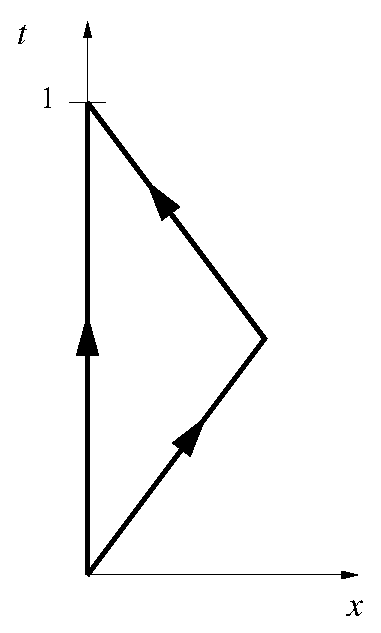
\includegraphics[height=6cm]{gravity_and_geometry/trip.eps}
\caption{Two ways of taking a spacetime trip.}
\label{fig:trip}
\end{center}   
\end{minipage}
\hfill
\begin{minipage}[t]{6.3cm}
\begin{center}
\includegraphics[height=6cm]{gravity_and_geometry/trip2.eps}
\caption{Two ways of taking a different spacetime trip.}
\label{fig:trip2}
\end{center}
\end{minipage}
\end{figure}

Let's see if this principle, which we call the {\em principle of
maximum proper time}, can be generalized.  For example, suppose we
want to go from the point $x = 0$, $t = 0$ to the point $x = 0.6$, $t
= 1$.  If our principle is correct then we should expect that the way
to take the trip in the greatest proper time is to go the `natural'
way, i.e., at a constant velocity $v = 0.6 c$, shown as route (a) in
Fig.~\ref{fig:trip2}.  We already know that the proper time for this
constant velocity trip is $(1 -0.6^2)^{1/2} = 0.8\, \mbox{s}$.  Can we
find a way that gives a longer proper time?
        
Figure \ref{fig:trip2} shows an alternate route to get to $x = 0.6$,
$t = 1$, labeled as path (b).  In homework problem \ref{prob:trip},
you will calculate the proper time for this route.  What you should
find is that the total proper time is less for the two-step trip,
route (b), than the 0.8 second `natural' trip at a single velocity,
route (a).  In fact there is no other route that gives a longer proper
time than the natural route.  Our principle shows an encouraging
ability to ``explain'' Newton's first law, the law of inertia.

This same principle works in curved spacetime.  The path between two
events actually taken by a freely falling body is that path that
MAXIMIZES the elapsed proper time.  This rule leads to the
``straightest'' possible path through the curved spacetime, and
answers the question:  How is it that ``spacetime tells mass how to
move''?

\begin{figure}[t]
\begin{center}
\includegraphics[width=4in]{gravity_and_geometry/trajectory.pdf}
\end{center}
\caption{Trajectories}
\label{fig:trajectories}
\end{figure}
     
Here is a qualitative example.  Throw a ball straight up and catch it
one second later at the same original height.  What is the ``naturally
chosen'' path through spacetime that maximizes proper time?  We have
just seen that, because of time dilation, paths that speed up, slow
down, or reverse direction tend to \textit{decrease} proper time.  On
the other hand, we've learned that clocks at higher altitudes measure
\textit{more} elapsed proper time than those at lower altitudes.  So
now consider these three paths, shown in Fig.~\ref{fig:trajectories}:

\begin{description}
\item[Path 1] The ball stays just above your hand the whole time.  No
  speeding to decrease proper time --- BUT also not taking advantage of
  increasing proper time by going high where clocks run faster.   Not
  the best.

\item[Path 2] Zoom high at almost light-speed, zoom back down.  This
  gets the ball high where clocks run fast, but time dilation at near
  light speed means almost no elapsed proper time!  No good.

\item[Path 3] Spend most of the trip at a higher place where proper
  time elapses rapidly.  But don't go very fast or change speed
  quickly, so the time dilation is not too severe.
\end{description}
        
Result: Best path for maximizing proper time is parabolic motion ---
fast up, slow and stop smoothly at the top, faster on the way down.
This is the motion we actually observe!

\newpage     

\section*{Problems}
\markright{PROBLEMS}

\begin{problem}
  Refer to Fig.~\ref{fig:sphere}.  Suppose $C_1$ is the $50^\circ$
  north latitude circle on the earth, and $C_2$ is the $40^\circ$
  north latitude circle on Earth.  The measured circumferences are
  $C_1 = 25850\, \mbox{km}$ and $C_2 = 30800\, \mbox{km}$.
  \begin{enumerate}
  \item Determine $r_1$, $r_2$ and $\Delta r$.
  \item Determine $\Delta s$ as a direct measurement on the earth's surface
    of the distance between the $40^\circ$ and $50^\circ$ latitude
    circles.  Compare your result to $\Delta r$.
  \item Explain how you could use your results to convince a member of
    the Flat Earth Society that the earth's surface is actually
    curved.
  \end{enumerate}
  \label{prob:sphere}
\end{problem}


\begin{problem}
  Consider clock $C$ on the surface of a neutron star, and clock $D$
  far away.  How do their rates compare?  How much time elapses on
  clock $D$ before clock $C$ is one second behind?  (The mass and
  radius of the neutron star are $2\times 10^{30}\units{kg}$ and
  $10\units{km}$, respectively.)
  \label{prob:neutron_star_time}
\end{problem}

\begin{problem}
  For the same neutron star as in
  Problem~\ref{prob:neutron_star_time}, calculate the height above
  the surface for which the circumference of a circle concentric with
  the star is $2\pi\times 10.001\units{km}$.
  \label{prob:neutron_star_space}
\end{problem}


\begin{problem}
  Following path (b) in Fig.~\ref{fig:trip2} means you go at $v =
  0.8c$ for the first leg, and $v = 0$ for the next.  Calculate the
  $t$-coordinate at the junction point; then determine the proper time
  for each leg and add them to get the total proper time.  Compare to
  the $0.8\, \mbox{s}$ of the direct route.
  \label{prob:trip}
\end{problem}



\chapter*{Answers to Selected Problems}
\addcontentsline{toc}{chapter}{Answers to Selected Problems}
\markboth{ANSWERS}{ANSWERS}

\noindent {\bf Additional Problems}

\noindent {\bf A\ref{prob:falling_birdie}}~(a)~$v_{\rm terminal} = g/b$.  
{\bf A\ref{prob:rocket_motion}}~$130\units{m/s}$; $18\units{m/s$^2$}$. 
{\bf A\ref{prob:blow_dart}}~(a)~$v_{\rm avg} = 0$.
{\bf A\ref{prob:spring_forward}}~$v =\sqrt{kx_0^2/m - 2 gx_0}$; $h = kx_0^2/2mg$. 
{\bf A\ref{prob:skiing}}~(d)~$\sqrt{gR}$; (e)~$2.5R$; (f)~$6mg$.
{\bf A\ref{prob:trapped}}~(a)~$6\units{km}$; (b)~$2\units{kJ}$; c)~drifts 
as far as ${\sim}7\units{km}$. 
{\bf A\ref{prob:hogwarts}}~(a)~$2.7\units{m/s}$; (b)~$2.7\units{m/s}$; 
c)~$2.7\, \mbox{m/s}$.  
{\bf A\ref{prob:photon_absorption}}~$m = 1718\units{MeV/$c^2$}$; $u = 0.4c$.  
{\bf A\ref{prob:light}}~$550\units{MeV/$c^2$}$. 
{\bf A\ref{prob:ball_turns}}~(a)~$0.085\units{J}$; (b)~more kinetic energy 
($0.141\units{J}$); 
(c)~$347\units{rev/min}$.\\
 {\bf A\ref{prob:cycle}}~(a)~$82^\circ\units{C}$ or $355\units{K}$; 
(b)~$A\to B$:~$1873\units{J}$, $B\to C$:~$0\units{J}$, 
$C\to A$:~$-1701\units{J}$; (c)~0.092; d)~0.355.
{\bf A\ref{prob:pulleywithmass}}~$a = g(m_2-m_1)/(m_1+m_2+m_3/2)$, downward
for $m_2$.
{\bf A\ref{problem:gravity_earth_on_moon}}~(a)~$0.0027\units{N/kg}$; 
(b)~$2.0\times 10^{20}\units{N}$; (c)~$0.19\units{N}$.\\
{\bf A\ref{prob:nonuniform_rod}}~(a)~$m=C(L_2^2-L_1^2)/2$; (b)~$GC\ln(L_2/L_1)$.
{\bf A\ref{problem:static_friction}}~$T\cos\theta$.
{\bf A\ref{problem:W-KE-baseball}}~(a)~+23.52\units{J}; (b)~$14.3\units{m/s}$.
%{\bf A\ref{problem:recoil_on_ice}}~$0.24\units{m/s}$.
{\bf A\ref{problem:simple_angmom}}~$\vec{L}_A = -31.5\, 
\hat{k}\units{kg$\cdot$m$^2$/s}$, $\vec{L}_B = 0$,
$\vec{L}_C = +15.75\, \hat{k}\units{kg$\cdot$ m$^2$/s}$.  
{\bf A\ref{problem:blarg_dimensions}}~(c) and (f) are possible; the others
have incorrect dimensions.
{\bf A\ref{problem:ratios_trafficandpizza}}~(a) 197 cars; (b) \$22.22.
{\bf A\ref{problem:asteroid}}~$7.4\units{y}$.
{\bf A\ref{problem:Jupiter_Moons}}~$7.3\units{d}$.
\medskip

\noindent {\bf Chapter \ref{chapter:numerical}}

\noindent 
{\bf \ref{chapter:numerical}.\ref{problem:ho-undamped-num}}~(a)~$x(2) 
= 7.0\units{m}$, $v(2)=-2.9\units{m/s}$; (b)~$x(2) = 6.56\units{m}$, 
$v(2)=-2.80\units{m/s}$.
\medskip

\noindent {\bf Chapter \ref{chapter:relativityI}}

\noindent 
{\bf \ref{chapter:relativityI}.\ref{prob:rel_units}}~$0.133\units{lt-s/s}$.  
{\bf \ref{chapter:relativityI}.\ref{prob:rel_units2}}~$1.8\times 10^7\units{m/s}$.  
{\bf \ref{chapter:relativityI}.\ref{prob:time_dilation1}}~$0.995\units{lt-s/s} 
= 2.98\times 10^8\units{m/s}$.  
{\bf \ref{chapter:relativityI}.\ref{prob:meteorite}}~$5.92\times 10^5\units{s}$.
{\bf \ref{chapter:relativityI}.\ref{prob:alpha_centauri}}~(a)~$6\frac{2}{3}
\units{yr}$; (b)~$5\frac{1}{3}\units{yr}$; 
(c)~$3.2\units{lt-yr}$; (d)~$3.2\units{lt-yr}$.\\ 
{\bf \ref{chapter:relativityI}.\ref{prob:alpha_centauri2}}~(a)~$4.47\units{yr}$; 
(b)~$0.894c$. 
{\bf \ref{chapter:relativityI}.\ref{prob:betelgeuse}}~(a)~$48\units{lt-yr}$; 
(b)~$0.958c$.
{\bf \ref{chapter:relativityI}.\ref{prob:terns}}~(a)~$20\units{ms}$; 
(b)~$9.6\units{lt-ms}$. 
{\bf \ref{chapter:relativityI}.\ref{prob:catch_on_trainI}}~(a)~$0.50\units{s}$;
(b)~$0.50\units{s}$ (Duh!); (c)~$15.8\units{m}$; (d)~$31.6\units{m/s}$;
{\bf \ref{chapter:relativityI}.\ref{prob:catch_on_trainII}}~$26.0\units{m/s}$.
\medskip

\noindent {\bf Chapter \ref{chapter:relativistic_spacetime}}

\noindent
{\bf \ref{chapter:relativistic_spacetime}.1}~Yes;
{\bf \ref{chapter:relativistic_spacetime}.\ref{prob:spacetimeII}}~(a)~A; 
(b)~B; (c)~D, (d)~b,c,d; (e)~a,e; (f)~space-like: bc, bd, cd, ae, be, ce; 
time-like: ab, ac, de.
{\bf \ref{chapter:relativistic_spacetime}.\ref{prob:solar_flare}}~(a)~calendar 
page; (b)~B, then C, then A; (c)~$\Delta t_{\rm BA,Earth} = 18\units{min}$, 
$\Delta t_{\rm AC,Earth} = 10\units{min}$, $\Delta t_{\rm BC,Earth} = 
8\units{min}$; 
(d)~$30\units{min}$; 
(e)~BC light-like, CA time-like, AB time-like. 
%{\bf \ref{chapter:relativistic_spacetime}.\ref{prob:evil_genius}}~(a,b)~calendar page; 
%(c)~$0.172c$;
%(d)~$7.25\units{min}$.
% {\bf \ref{chapter:relativistic_spacetime}.\ref{prob:cosmic_ray}}~(b)~$1.98\units{lt-$\mu$s}$; 
% (c)~$14.2\units{$\mu$s}$, $14.1\units{lt-$\mu$s}$.  
{\bf \ref{chapter:relativistic_spacetime}.\ref{prob:farmer}}~(a)~$12\units{lt-ns}$, yes;
(b)~$9.6\units{lt-ns}$, no; (c)~discuss with prob session group and instructor; 
(d)~A, C, B, D; it should be consistent with (a);
(e)~A, B, C, D; it should be consistent with (b);
(f)~Discuss with problem session group and instructor.
{\bf \ref{chapter:relativistic_spacetime}.\ref{prob:two_ships}}~(b)~$6\units{lt-s}$; (c)~$2\units{lt-s}$; (d)~$10\units{lt-s}$;
(e)~$14\units{s}$.
{\bf \ref{chapter:relativistic_spacetime}.\ref{prob:sparkler}}~(a)~$80\units{lt-s}$; 
(b)~$80\units{lt-s}$, $0.8\units{lt-s/s}=0.8c$; 
(c)~$0.8\units{lt-s/s}=0.8c$, $48\units{lt-s}$.
{\bf \ref{chapter:relativistic_spacetime}.\ref{prob:spacetimeIII}}~(b)~$0.8c$; 
(c)~$4.5\units{yr}$; 
(d)~$3.6\units{lt-yr}$; (f)~D, B, C, A; (g)~C, D, B, A; 
(h)~$4.58\units{lt-yr}$.
\medskip


\noindent {\bf Chapter \ref{chapter:relativity_pande}}


\noindent
{\bf \ref{chapter:relativity_pande}.\ref{prob:vtransform}}~$0.308c$.
{\bf \ref{chapter:relativity_pande}.\ref{prob:vtransform2}}~$0.385c$ or 
$0.946$.
{\bf \ref{chapter:relativity_pande}.\ref{prob:energy-to-accelerate}}~$1.05\units{MeV}$. 
%{\bf \ref{chapter:relativity_pande}.\ref{prob:electrons}}~Each answer 
%lists $E$, $K$, $p$, and $u$: 
%(a)~$1.0\units{MeV}$, $0.489\, \units{MeV}$, $0.860\, 
%\units{MeV/$c$}$, $0.860c$;
%(b)~$0.761\units{MeV}$, $0.25\units{MeV}$, $0.564\units{MeV/$c$}$, $0.740c$;
%(c)~$1.261\units{MeV}$, $0.75\units{MeV}$, $1.153\units{MeV/$c$}$, $0.914c$;
%(d)~$1.123\units{MeV}$, $0.612\units{MeV}$, $1.0\units{MeV/$c$}$, $0.890c$.
{\bf \ref{chapter:relativity_pande}.\ref{prob:proton}}~$p = 6499\units{MeV/$c$}$, $u = 0.9897c$.
{\bf \ref{chapter:relativity_pande}.\ref{prob:ep_transform}}~$E^\prime = 
15\units{MeV}$, $p^\prime = 12\units{MeV/$c$}$.
{\bf \ref{chapter:relativity_pande}.\ref{prob:fermilab}}~(a)~$899\units{GeV}$; 
(b)~$100\units{GeV}$; 
(c)~$u/c \simeq 1 - 8.98\times 10^{-9} \simeq 0.999999991$.
{\bf \ref{chapter:relativity_pande}.\ref{prob:J}}~$p = 200\units{MeV/$c$}$; 
$K = 100\units{MeV}$.
{\bf \ref{chapter:relativity_pande}.\ref{prob:fermilab2}}~$p = 1.921\units{GeV/$c$}$; $u = 0.899c$.
\medskip

\noindent {\bf Chapter \ref{chapter:relativity_app}}

\noindent
{\bf \ref{chapter:relativity_app}.\ref{prob:rel_recoil}}~(c)~$E_1 = 
10/\sqrt{5} \simeq 4.47\units{GeV}$, 
$p_3 = 10/\sqrt{5} \simeq 4.47\units{GeV/$c$}$.
{\bf \ref{chapter:relativity_app}.\ref{prob:rel_recoil2}}~$u = 2c/3$, 
same magnitude as Example \ref{ex:nuclear_decay}.
%{\bf \ref{chapter:relativity_app}.\ref{prob:pair_creation}}~$E_{\rm initial}
%=940\units{MeV}$.
{\bf \ref{chapter:relativity_app}.\ref{prob:composite}}~(a)~$m = 
5.06\units{MeV/$c^2$}$, $u = 0.19c$; (b)~$0.06\units{MeV}$.
%{\bf \ref{chapter:relativity_app}.\ref{prob:deuteron}}~$2.23\units{MeV}$.
{\bf \ref{chapter:relativity_app}.\ref{prob:fusion}}~(a)~rest energy to 
kinetic energy; (b)~$17.6\units{MeV}$.
\medskip


%\noindent {\bf Chapter \ref{chapter:stat-mech}}

%\noindent
%{\bf \ref{chapter:stat-mech}.\ref{prob:micro-calc}}~$W = 7560$. 
%{\bf \ref{chapter:stat-mech}.\ref{prob:w_ratio}}~$W^\prime/W = 4.79$.
%{\bf \ref{chapter:stat-mech}.\ref{prob:equilibrium}}~$n_2 \simeq 4050$.
%{\bf \ref{chapter:stat-mech}.\ref{prob:systemsAB}}~(a)~A; (b)~A to B; 
%(c)~$(W_A^\prime W_b^\prime)/(W_AW_B)~\simeq 1.02$.
%{\bf \ref{chapter:stat-mech}.\ref{prob:new_macrostate}}~$\{ 4,1,3,0,2,0,\dots\}$.
%{\bf \ref{chapter:stat-mech}.\ref{prob:exhaustive_list}}~(a)~$W = 1$ for 
%\ref{fig:levels_e3}~(a), $W=3$ for \ref{fig:levels_e3}(b).


\noindent {\bf Chapter \ref{chapter:thermal_energy}}

\noindent 
{\bf \ref{chapter:thermal_energy}.\ref{problem:flattium}}~$2nRT$.
{\bf \ref{chapter:thermal_energy}.\ref{problem:ball-spring_iron}}~(a)~$m=9.27
\times 10^{-26}\units{kg}$, $d=2.28\times 10^{-10}\units{m}$, 
$k_\text{sp}=48.0\units{N/m}$; (b)~5180\units{m/s}.
%{\bf \ref{chapter:thermal_energy}.\ref{problem:compare_iron_copper}}~(a)~equal, (b)~iron.
{\bf \ref{chapter:thermal_energy}.\ref{problem:iron_E_thermal}}~9.30\units{kJ}.
{\bf \ref{chapter:thermal_energy}.\ref{problem:mole_kg_cc}}~(a)~628\units{J}; 
(b)~11.2\units{J}; (c)~88.5\units{J}.
{\bf \ref{chapter:thermal_energy}.\ref{problem:calorimetry}}~(a)~$30^\circ\units{C}$; (b)~499\units{J}.
%{\bf \ref{chapter:thermal_energy}.\ref{problem:iron_oscillation}}~$2.76\times 10^{-13}\units{s}$.
{\bf \ref{chapter:thermal_energy}.\ref{problem:falling_brick}}~$0.229^\circ\units{C}$.
%{\bf \ref{chapter:thermal_energy}.\ref{problem:silver_ball-spring}}~$\rho=10.4\units{g/cm$^3$}$,
%$Y=83\units{GN/m$^2$}$.
{\bf \ref{chapter:thermal_energy}.\ref{problem:heat_examples}}~b, e.
%{\bf \ref{chapter:thermal_energy}.\ref{problem:compare_heat_capacity}}~aluminum, copper, lead.
{\bf \ref{chapter:thermal_energy}.\ref{problem:thermal_energies_large}}~303,000 \units{J} versus 157 \units{J} (the word ``wow!'' would be appropriate here).
{\bf \ref{chapter:thermal_energy}.\ref{prob:polish_ring}}~223 \units{J}.
\medskip


\noindent {\bf Chapter \ref{chapter:liquids_and_gases}}

\noindent
{\bf \ref{chapter:liquids_and_gases}.\ref{problem:iron_melting}}~(a)~$9.2\times 10^{-12}\units{m}$; (b)~$1810
\units{K}$.
%%{\bf \ref{chapter:liquids_and_gases}.\ref{problem:sesame_street}}~water.
{\bf \ref{chapter:liquids_and_gases}.\ref{problem:thermal_speeds}}~(a)~$479
\units{m/s}$; (b)~$678\units{m/s}$; (c)~$409\units{m/s}$.
{\bf \ref{chapter:liquids_and_gases}.\ref{problem:water_calorimetry}}~(a)~$n_\text{ice}=5.6\units{mol}$, $n_\text{liq}=11.1\units{mol}$; 
(b)~$20.9\units{kJ}$, (c)~$3.5\units{mol}$.
{\bf \ref{chapter:liquids_and_gases}.\ref{problem:ideal_gas_ratios}} 
(Note:  assume $m_1 = m_2$.) ~(a)~$\sqrt{2}$; (b)~2, (c)~2.
{\bf \ref{chapter:liquids_and_gases}.\ref{problem:ideal_gas_moles}}~$0.194\units{mol}$.
%{\bf \ref{chapter:liquids_and_gases}.\ref{problem:heat_of_vaporization}}~(a)~Oxygen~9.1, 
%Nitrogen~8.6, Water~13.1, Lead 10.7, Copper 12.7, Iron 13.1, rule of thumb 12,
%(b)~$5.15\times 10^{-21}\units{J}$ or $0.032\units{eV}$.
%{\bf \ref{chapter:liquids_and_gases}.\ref{problem:speed_of_sound}}~926\units{m/s}.
{\bf \ref{chapter:liquids_and_gases}.\ref{problem:aquaman}}~$2.44\units{atm}$.
{\bf \ref{chapter:liquids_and_gases}.\ref{problem:ideal_gas_quant}}~(a)~$4.76
\times 10^{-23}\units{kg$\cdot$m/s}$; (b)~2,560 collisions/s; (c)~$1.22\times
10^{-19}\units{kg$\cdot$m/s}$; (d)~$1.22\times 10^{-19}\units{N}$;
(e)~$1.01\times 10^3\units{N}$; (f)~$1.01\times 10^5\units{Pa}$.
\medskip

\noindent {\bf Chapter \ref{chapter:second_law}}

\noindent
{\bf \ref{chapter:second_law}.\ref{prob:multiplicityforthree}}~(a)~15.
{\bf \ref{chapter:second_law}.\ref{prob:mult_of_twentyfour}}~$1.5 \times 10^{10}$.
{\bf \ref{chapter:second_law}.\ref{prob:rolldie}}~(a) 1/216; (b)~1/216; 
(c)~10/216.
{\bf \ref{chapter:second_law}.\ref{prob:twosolids}}~$25/7 \simeq 3.6$.
{\bf \ref{chapter:second_law}.\ref{prob:tempoflargeobject}}~$300\units{K}$.
{\bf \ref{chapter:second_law}.\ref{prob:diminishing}}~(a)~$0.916 k_B$; 
(b)~$0.446 k_B$.
{\bf \ref{chapter:second_law}.\ref{prob:entropyoftwosolids}}~$E_{A,f}=4E_{B,f}$
{\bf \ref{chapter:second_law}.\ref{prob:strangesystem}}~(a)~From A to B; 
(b)~All energy will flow to system B.
{\bf \ref{chapter:second_law}.\ref{prob:energy_transferA}}~(a)~From A to B;
(b) $\Delta S_A = -0.6\units{J/K}$, $\Delta S_B = +1.20\units{J/K}$, 
$\Delta S_{\rm total} = +0.6\units{J/K}$;\\
(c) $\Omega_{\rm after}/\Omega_{\rm before} = e^{4.35\times 10^{22}}$.
 
\medskip

\noindent {\bf Chapter \ref{chapter:heat_engines}}

\noindent
{\bf \ref{chapter:heat_engines}.\ref{prob:iceintowater}}~(a)~$1.38\units{mol}$ 
melted; (b)~$+30.3\units{J/K}$; (c)~$-29.2\units{J/K}$; yes (it had 
{\bf better} be consistent with the second law!)
{\bf \ref{chapter:heat_engines}.\ref{prob:multiplicityformelting}}~this is 
$e$  raised to the power $1.59\times 10^{24}$.  (Don't bother trying to 
calculate that with your calculator.)
{\bf \ref{chapter:heat_engines}.\ref{prob:simpleengine}}~1/2.
{\bf \ref{chapter:heat_engines}.\ref{prob:onebrickengine}}~(a)~$-131.5\units{J/K}$; 
(b)~$38.8\units{kJ}$; (c)~0.241.
{\bf \ref{chapter:heat_engines}.\ref{prob:twobrickengine}}~$358\units{J}$ 
(Note:  this assumes you keep enough digits in the final temperature.  
If you round the final temperature to $346\units{K}$, you'll get 
$399\units{J}$).
{\bf \ref{chapter:heat_engines}.\ref{prob:threelegcycle}}~(a)~A:  
$100\units{kPa}$, $22.7\units{L}$, $273\units{K}$; B: $155\units{kPa}$, 
$22.7\units{L}$, $423\units{K}$; C: $100\units{kPa}$, $29.5\units{L}$, 
$355\units{K}$; (b)~A to B:  $1870\units{J}$; B to C:  0; C to A:  
$-1700\units{J}$; (c)~0.092.
{\bf \ref{chapter:heat_engines}.\ref{prob:rectangularcycle}}~(a)~$T_H = 
4813\units{K}$, $T_C = 289\units{K}$; (b)~$\epsilon = 0.18$, as 
compared with maximum of 0.94.

\medskip
\newpage

\noindent {\bf Chapter \ref{chapter:gravity}}

\noindent
{\bf \ref{chapter:gravity}.\ref{prob:sphere}}~(a)~$r_1 = 4114\units{km}$, 
$r_2 = 4902\units{km}$, $\Delta r = 788\units{km}$; (b)~$1112\units{km}$;
(c) $\Delta s \ne \Delta r$, which means it is curved.
{\bf \ref{chapter:gravity}.\ref{prob:neutron_star_time}~(a)~$\Delta \tau _C = 0.839\Delta \tau _D$; $6.20$ s.
{\bf \ref{chapter:gravity}.\ref{prob:neutron_star_space}~$1.19$ m

%{\bf \ref{chapter:gravity}.\ref{prob:clock_rate}}~$1.1\times 10^{-13}$.
%{\bf \ref{chapter:gravity}.\ref{prob:trip}}~$0.75\units{s}$; $0.70\units{s}$.
%{\bf \ref{chapter:gravity}.\ref{prob:circlesonearth}}~(a)~$2\pi R_E 
%\frac{90^{\circ}-\theta}{360^{\circ}}$; (b)~$R_E\cos\theta$; 
%(c)~$1.57R_E$, $R_E$; (d)~$0.175R_E$, $0.174R_E$.


%\chapter*{Tables of Thermodyamic Properties}
%\cleardoublepage
\phantom{Nada}
%\vfill
%\centering \tiny \emph{This page unintentionally  left blank}
\newpage
\begin{center}
\Large \textbf{
Tables of Thermodynamic Properties}
\end{center}
\addcontentsline{toc}{chapter}{Tables of Thermodynamic Properties}
\markboth{Thermodynamic Properties}{Thermodynamic Properties}


%\begin{table}[h]
\begin{center}
\textbf{Selected Properties of Solids}\\ \smallskip
\begin{tabular}{lccccc}
\hline\hline
Material & $M$ (g/mol) & $\rho$ (g/cm$^3$) & $Y$ (GN/m$^2$) & 
$C$ (J/mol$\cdot$K)  & $v_s$ (m/s) \\ \hline
% & (g/mol) & (g/cm$^3$) & (GN/m$^2$) & (J/mol$\cdot$K) & (m/s)\\ \hline
Aluminum & 27.0 & 2.70 & 70  & 24.2  & 5000\\
Iron     & 55.8 & 7.87 & 211 & 25.1  & 5120\\
Copper   & 63.5 & 8.96 & 130 & 24.4  & 3810\\
Gold     & 197  & 19.3 & 78  & 25.4  & 2030\\
Lead     & 207  & 11.3 & 16  & 26.6  & 1190\\
ideal solid & $mN_A$ & $m/d^3$ & $k_{\rm sp}/d$ & 3R = 24.9  
                                          &  $d\sqrt{k_{\rm sp}/m}$\\
\hline\hline
\end{tabular}
%\caption{Material properties for a few selected substances.}

% \begin{tabular}{lccccc}
% \hline\hline
% Material & $M$ (g/mol) & $\rho$ (g/cm$^3$) & $Y$ (GN/m$^2$) & 
% $C$ (J/mol$\cdot$K)  & $v_s$ (m/s) \\ \hline
% % & (g/mol) & (g/cm$^3$) & (GN/m$^2$) & (J/mol$\cdot$K) & (m/s)\\ \hline
% Aluminum & 27.0 & 2.70 & 70  & 24.2  & 5000\\
% Iron     & 55.8 & 7.87 & 211 & 25.1  & 5120\\
% Copper   & 63.5 & 8.96 & 130 & 24.4  & 3810\\
% Gold     & 197  & 19.3 & 78  & 25.4  & 2030\\
% Lead     & 207  & 11.3 & 16  & 26.6  & 1190\\
% ideal solid & $mN_A$ & $m/d^3$ & $k_{\rm sp}/d$ & 3R = 24.9  
%                                           &  $d\sqrt{k_{\rm sp}/m}$\\
% \hline\hline
% \end{tabular}
%\caption{Material properties for a few selected substances.}
%\label{table:material_properties}
\end{center}
%\end{table}

%\bigskip\bigskip


\bigskip
%\begin{table}[h]

\begin{center}
\textbf{Liquid Specific Heats}\\ \smallskip
\begin{tabular}{llc}
\hline\hline
Liquid & molecule & $C$ (J/mol$\cdot$K) \\ \hline
\noalign{\smallskip}
water & H$_2$O & 75.3 \\
methanol & CH$_3$OH & 79.5 \\
ethanol & C$_2$H$_5$OH  &  112.4 \\
acetone & (CH$_3$)$_2$CO & 125.5 \\
benzene & C$_6$H$_6$ & 134.8 \\
\hline\hline
\end{tabular}
% \caption{Molar specific heats of selected liquids.  Data is taken at 
% room temperature.}

%\hspace{0.5in}

% \begin{tabular}{llc}
% \hline\hline
% Liquid & molecule & $C$ (J/mol$\cdot$K) \\ \hline
% \noalign{\smallskip}
% water & H$_2$O & 75.3 \\
% methanol & CH$_3$OH & 79.5 \\
% ethanol & C$_2$H$_5$OH  &  112.4 \\
% acetone & (CH$_3$)$_2$CO & 125.5 \\
% benzene & C$_6$H$_6$ & 134.8 \\
% \hline\hline
% \end{tabular}
% \caption{Molar specific heats of selected liquids.  Data is taken at 
% room temperature.}
%\label{table:liquid_specific_heats}
\end{center}
%\end{table}
%\vspace{0.2in}

\bigskip
%\begin{table}[h]
%\hspace{0.5in}

\begin{center}
\textbf{Gas Specific Heats}\\ \smallskip
\begin{tabular}{lcccc}
\hline\hline
Gas & Type & $C$ (J/mol$\cdot$K) \\ \hline
\noalign{\smallskip}
Neon (Ne) & monatomic & 12.5 \\
Argon (Ar) & monatomic & 12.5 \\
Hydrogen (H$_2$) & diatomic & 20.5 \\
Oxygen (O$_2$) & diatomic & 21.1 \\
Nitrogen (N$_2$) & diatomic & 20.8 \\
\hline\hline
\end{tabular}
% \caption{Molar specific heats (at constant volume) of selected gases.}


% \begin{tabular}{lcccc}
% \hline\hline
% Gas & Type & $C$ (J/mol$\cdot$K) \\ \hline
% \noalign{\smallskip}
% Neon (Ne) & monatomic & 12.5 \\
% Argon (Ar) & monatomic & 12.5 \\
% Hydrogen (H$_2$) & diatomic & 20.5 \\
% Oxygen (O$_2$) & diatomic & 21.1 \\
% Nitrogen (N$_2$) & diatomic & 20.8 \\
% \hline\hline
% \end{tabular}
% \caption{Molar specific heats (at constant volume) of selected gases.}
%\label{table:gas_specific_heats}
\end{center}

%\end{table}
%\vspace{0.2in}


\bigskip

%\begin{table}[h]
%\hspace{0.5in}
\begin{center}
\textbf{Latent Heats}\\ \smallskip
\begin{tabular}{lcccc}
\hline\hline
Material & $T_m$ (K) & $L_f$ (kJ/mol) & $T_v$ (K) & $L_v$ (kJ/mol) \\ \hline
\noalign{\smallskip}
Oxygen & 54.4 & 0.444 & 90.2 & 6.82 \\
Nitrogen & 63.2 & 0.72 & 77.4 & 5.56 \\
Ethanol & 159 & 5.02 & 352 & 38.6 \\
Water & 273 & 6.01 & 373 & 40.6  \\ 
Lead & 600 & 4.77 & 2022 & 180 \\
Copper & 1358 & 13.3 & 2835 & 300 \\
Iron  & 1811 & 13.8 & 3134 & 340 \\
\hline\hline
%\label{table:latent_heats}
\end{tabular}
% \caption{Melting and vaporization temperatures for a few materials, along
% with the latent heats of fusion and vaporization.}


% \begin{tabular}{lcccc}
% \hline\hline
% Material & $T_m$ (K) & $L_f$ (kJ/mol) & $T_v$ (K) & $L_v$ (kJ/mol) \\ \hline
% \noalign{\smallskip}
% Oxygen & 54.4 & 0.444 & 90.2 & 6.82 \\
% Nitrogen & 63.2 & 0.72 & 77.4 & 5.56 \\
% Ethanol & 159 & 5.02 & 352 & 38.6 \\
% Water & 273 & 6.01 & 373 & 40.6  \\ 
% Lead & 600 & 4.77 & 2022 & 180 \\
% Copper & 1358 & 13.3 & 2835 & 300 \\
% Iron  & 1811 & 13.8 & 3134 & 340 \\
% \hline\hline
% %\label{table:latent_heats}
% \end{tabular}
% \caption{Melting and vaporization temperatures for a few materials, along
% with the latent heats of fusion and vaporization.}
%\label{table:phase_transitions}
\end{center}
%\end{table}


\end{document}
